\chapter{Numerical Results}
\label{chapter 7}

\section*{Numerical validation of Projection methods}
In this section we will test the accuracy of the Projection methods as well as the Gauge method with analytical solutions. Interesting flow problems are also 
\section{Accuracy test}
There are many ways to test the accuracy of numerical schemes. One of the most popular way is to compare the numerical solution generated through computer simulation with analytical solutions. By calculating the error with appropriate norms (e.g. $L_1,\,L_2$ and $L_\infty$) this method provides precise measure on error and convergence rate. However in many real-life applications in fluid dynamics, analytical solution is often not known or difficult to compute and implement. This is often when mixed boundary conditions are imposed in a complex geometry. Then people usually run simulations and compare with experimental results which could be somewhat less quantitative. Another good way to test accuracy in such situations is using reference solutions done by previous researchers. It is worth to point that the reference solution is not the analytical solution to the test problem, rather it is a numerical solution generated in fine grids which is commonly accepted in literature. For instance, the lid driven cavity problem is such a simple test problem but retains many interesting flow physics. One of the commonly accepted reference solution is the ``Benchmark Spectral Results on the Lid-Driven Cavity Flow" done by \emph{O. Botella et al.} 1998 \cite{botella1998benchmark}.\\

For the purpose of accuracy and convergence test, we consider two simple 2-D flow problems with analytic solutions exists. This reveals more fundamental properties and error behaviours for the projection schemes.\\

\subsection{Forced flow}
The test problem is a forced flow example where the fluid is confined in a square domain $\Omega = [-1,1] \times [-1,1]$ and initially remains stationary. The flow is caused by an external driving force. This is one of the simplest settings to consider slip/no-slip boundary conditions. Homogeneous boundary condition (no - slip) is imposed on the four sides of the domain \\
($\partial \Omega:$ West: $x = -1$, East: $x=1$, South: $y = -1$, North: $y=1$).\\

The settings are summarised below:
\begin{equation}
\text{Analytical solution}
\begin{cases}
u = \pi\sin(t)\sin(2\pi y)\sin^2(\pi x) \text{   in $\Omega$} \\
v = - \pi \sin(t)\sin(2\pi x)\sin^2(\pi y) \text{   in $\Omega$} \\
p = \sin(t)\cos(\pi x)\sin(\pi y)  \text{   in $\Omega$}  \\
u_0 = u(t=0,x,y)  \text{   in $\Omega$}  \\
v_0 = v(t=0,x,y)  \text{   in $\Omega$}  \\
\end{cases}
\end{equation}
with homogeneous Dirichlet boundary condition:
\begin{equation*}
u(t, x=\pm 1, y) = u(t, x,y= \pm 1) = 0
\end{equation*}

It is augmented with a forcing term: $f = \partial_x\,\textbf{u} - \dfrac{1}{Re}\nabla^2 \textbf{u} + \nabla p$ to make the above ``solutions" valid. For simplicity we take the Reynolds number ($Re$) to be 1. By substituting our analytical solutions into $f$ we found the forcing term is given as:
\begin{equation}
f = 
\begin{cases}
fx = \pi\cos(t)\sin(2\pi y)\sin^2(\pi x) -  2 \pi^3\sin(t)\sin(2\pi y)\,(\cos(2\pi x) - 2\sin^2(\pi x)) \\
\,\,\,\,\,\,\,- \, \pi\sin(t)\sin(\pi y)\sin(\pi x) \text{   in $\Omega$} \\
fy = - \pi\cos(t)\sin(2\pi x)\sin^2(\pi y) - 2\pi^3\sin(t)\sin(2\pi x)\,(2\sin^2(\pi y) - \cos(2\pi y)) \\
\,\,\,\,\,\,\,+ \, \pi\sin(t)\cos(\pi x)\cos(\pi y)  \text{   in $\Omega$}  \\
\end{cases}
\end{equation}

Because we are mainly interested in investigating how the time discretisation error behaviours, hence we want the spatial discretisation error to be negligible compared to the time discretisation error, hence we need to take care of the spatial stepping ($\Delta x$) and time stepping ($\Delta t$). The CFL number is given as: $C = \dfrac{U\,\Delta t}{\Delta x}$ where $U = \pi$ is the absolute bound for velocity. For this problem, a range of CFL number were used including 5, 2, 1, 0.5, 0.1, 0.05 and 0.01. The effect of different CFL number on numerical results is also briefly discussed here. (\textbf{I will add this part soon})\\

The actual error $e_h$ is consisted of both spatial and temporal error and $h$ is just an index to indicate the grid size (e.g. a 120 $\times$ 120 grid).\\
In our purpose of testing the error behaviour in time, we want the temporal error to dominate and thus we can assume the following simplified error relation:\\
We expect the error is a function of $\Delta t$ and thus:
\begin{equation}
e_h = \Delta t^p
\end{equation}
where $p$ is the convergence rate (don't be confused with pressure) and in our case we want $p=2$.\\

The error $e_h$ is simply calculated by taking the difference between numerical and analytical solutions point-wisely. It is important to compare the solutions only under the same conditions, for instance grid size and end of time... Comparing solutions at different time would of course cause strange error behaviours!\\

By take logarithm on both side of the equation above we see that the logarithm of error in time has a linear relationship with the logarithm of time stepping ($\Delta t$). Thus the slope of the log error function should be the convergence rate.
\begin{equation}
log_{10} (e_h) = p\,log_{10} (\Delta t)
\end{equation}
Base 10 is used for simplicity, other bases including 2 and natural exponential works the same.\\

The strategy is follows: with the error of a coarse grid denoted as $e_h$. We half the spatial stepping ($\Delta x$) or equivalently double the grid size (e.g. from 15 $\times$ 15 to 30 $\times$ 30). Denoting the error of the finer grid as $e_{h_{1/2}}$. The time stepping at the meaning time is also halved. Then we look at how the error decreases. If our numerical scheme is second order accurate then the error should decrease by a factor of 4 going from the coarser grid to the finer grid.\\
This is easy to see by taking the ratio between the errors and using equation (6.3)
\begin{equation*}
\dfrac{e_h}{e_{h_{1/2}}} = \dfrac{\Delta t^2}{(\dfrac{1}{2}\Delta t)^2} = \dfrac{\Delta t^2}{\Delta t^2}\,\dfrac{1}{(\dfrac{1}{2})^2} = 4
\end{equation*}

A Log-Log plot of the error function is then generated and the convergence rate is finally extracted as the slope of the log error function.\\

It is important to specify the error norm as noted by many researchers that different norms could generated different convergence rates! \cite{pyo2005normal,guermond2004error}\\
In our analysis 3 commonly used norms were implemented: $L_1,\,L_2,\,L_\infty$. Each could reveals certain aspect of error behaviour. By combing the results generated using these 3 norms, a comprehensive analysis of convergence rate can be obtained.\\

We take the normalised $L_1$ norm and it is defined as:
\begin{equation}
||\,e^n\,||_{L_1} = \dfrac{1}{K}\,\sum^K_{k=0}\,|e^n_k|
\end{equation} 
where $e^n$ is the error field measured at step $n$ and $K$ is the dimension or size of the error field. For instance a $15 \times 15$ grid would corresponds to $K = 15^2$.\\

similarly we define the $L_2$ norm to be:
\begin{equation}
||\,e^n\,||_{L_2} = \left(\dfrac{1}{K^2}\,\sum^K_{k=0}\,|e^n_k|^2\right)^{1/2} = \dfrac{1}{K}\left(\sum^K_{k=0}\,|e^n_k|^2\right)^{1/2}
\end{equation}

and $L_\infty$:
\begin{equation}
||\,e^n\,||_{L_\infty} = \max_{\,\,\,0 \leq k \leq K\,\,\,}\,|e^n_k|
\end{equation}

To achieve optimal result, there are a number of thins that need to be considered. \\
First, since we are aiming to investigate the temporal error and hence we need to use fine grids to ensure the spatial error is negligible. Hence we have run the solvers up to grid size of $480 \times 480$. Higher grid numbers are also possible but takes very long time to compute. For completeness we have also included the results for small to moderate grids. Overall we have 6 data points corresponding to grid size of 15, 30, 60, 120, 240 and 480.\\

Second, smooth analytical solutions are also critical in obtaining optimal results. To qualify for smoothness we generally require the analytic velocity and pressure solutions are at least second order differentiable. The forced flow problem we presented here clearly satisfies this. Nevertheless, it is worth to point out that non-smoothness or even discontinuities would decrease the accuracy because this could prevent the numerical solution to converge to the correct solution. This problem is even exaggerated if the discontinuity happens at the boundary. For instance the driven cavity example we shall see in the next section. \textbf{I wil try to finish this section soon, I just need to add a few more plots})\\

In addition, care must also be taken to the pressure gradient along the boundary. We need to make sure the normal pressure gradient is non-zero along the boundary so that the accuracy performance can be distinguished between projection method $Pm\,1\,(a)$ and $Pm\,1\,(b)$. Recall $Pm\,1\,(a)$ has a non-physical zero Neumann boundary condition for the pressure variable and it is this drawback which causes the formation of numerical boundary layers.\\
Luckily, for our forced flow solution, the normal pressure gradient is non-zero along the North and South boundaries ($y = \pm 1$) (whereas it is zero along the other two boundaries)
\begin{equation*}
\text{North (South):}\, \textbf{n}\cdot \nabla p |_{y = \pm 1} = \partial_y\,p |_{y = \pm 1} = \mp \pi sin(t)\,cos(\pi x)
\end{equation*}

\begin{equation*}
\text{and East (West):}\,\textbf{n}\cdot \nabla p |_{x = \pm 1} = \partial_x\,p |_{x = \pm 1} = 0
\end{equation*}

With the above conditions all satisfied, we can now finally test our numerical solutions!\\

We have run simulations for Projection methods: $Pm\,1\,(a)$, $Pm\,1\,(b)$ and $Pm\,2$ as well as the Gauge method for a number of test runs with grid size ranges from $15 \times 15$ to $480 \times 480$.\\

As for a start, we run the simulations at $t = 1$ with the spatial domain: $[-1,1]^2$ and homogeneous Dirichlet boundary conditions imposed on velocities.\\

The exact and numerical solutions are summarised in Figure 6.1. The numerical solution is computed by $Pm\,1\,(b)$ with grid size: $60 \times 60$ and $CFL = 0.1$. This time, the numerical solutions seem to do a good job in approximating the true solutions. These ``nice" graphs however do not reveal much about the error behaviours. Hence let's take a look at the convergence rates instead. The rates for Projection methods are summarised in Figure 6.4 to 6.6. \\

It is obvious that the velocities are converging at an optimal 2nd order rate in all projection methods (see Figure 6.4 (a), 6.5 (a) and 6.6 (a)).\\

The pressure errors are a little worrying. First convergence are achieved for small to moderate grids ($15 \times  15$ to $60 \times 60$) whereas for finer grids the error starts to saturate or even increases (e.g. for grids higher than $120 \times 120$). Taking smaller CFL numbers (0.05 and 0.01) did not help to resolve this problem. Taking a closer look at the errors for individual grid sizes, we observed that the $L_1$ and $L_2$ are small compared to $L_\infty$ in general. This implies that numerical boundary layers have formed and they are smoothed out by $L_1$ and $L_2$ error norms. There is a sudden drop of $L_1$ and $L_2$ error norms going from grid size of 30 to 60 and then increased going from grid size 60 to 120. The errors are now comparable between all norms at this fine grid which implies that the error at interior points are suddenly increased. This suggests that the numerical solutions could either diverges to the reference solution or are converging to a different one. We first hypotheses that this is due to the limitation of our linear system solvers or even a bug in my code! However this was shown not the case, the cause of this problem is more mathematical and we will explain this shortly.\\

For now the convergence rates shown in Figure 6.4 - 6.6 were calculated excluding the outliers (at grid size of 120) and focus on the grid sizes from 15 to 60.\\
For $Pm\,1\,(a)$ strong deterioration in pressure error convergence is observed with a convergence rate of about 1.5 order ($L_1:\,  1.5883$ and $L_2: \, 1.8936$). In particular the $L_\infty$ norm was strongly deteriorated to first order accuracy:$ 1.1228$. This indicates that larger errors must have occurred and they are better picked up by $L_\infty$ norm. \\

To investigate further, let's take a look at the Error field shown in Figure 6.7 (a). The error field shows very interesting structure where it is almost flat in the interior but then the error quickly develops along the boundary. In particular along the ``South" ($y = 0$) and ``North" ($y=1$) boundary, thick numerical boundary layer is observed. This numerical boundary layer is probably due to the inconsistent pressure update formula for $Pm\,1\,(a)$. Recall that the numerical pressure satisfies a zero Neumann boundary condition and because of the square domain we work with have:
\begin{equation*}
\textbf{n} \cdot \nabla p^{n+1/2} |_{y=\pm 1} = \partial_y p^{n+1/2} |_{y=\pm 1} = 0
\end{equation*} 
The true pressure gradient is however very different:
\begin{equation*}
\partial_y P^{n+1/2} |_{y=\pm 1} = \pi sin((n+\dfrac{1}{2})\Delta t)
\end{equation*}
which is evidently non-zero.\\

Therefore the pronounced boundary layer in $Pm\,1\,(a)$ inevitably decrease the convergence rate especially in $L_\infty$ because it picks up the large singularities better. The boundary layers on the other hand seems to be partially smoothed out by the $L_1$ and $L_2$ norms because there is a sort of averaging process in the calculations. \\

In summary the degradation in accuracy for $Pm\,1\,(a)$ is evident. This is consistent with our hypothesis and also matches with the findings from other authors like \emph{David, Strikwerda and Shen et al}. \cite{brown2001accurate, strikwerda1999accuracy, guermond2006overview, guermond2004error}.\\

As for $Pm\,1\,(b)$, the accuracy is certainly better than that of $Pm\,1\,(b)$ because the pressure gradient along the boundary is more consistent. From Figure 6.7 (b), the numerical boundary layer is reduced significantly both in magnitude and in shape. However we still observed 4 large singularities at the corners. This suggests that the new update formula do seem to filter out the spurious mode. Hence from this point of view we have demonstrated that $Pm\,1\,(b)$ performs better than $Pm\,1\,(a)$\\

\begin{figure}[H]
	\centering
	\begin{subfigure}[t]{2.5in}
		\centering
		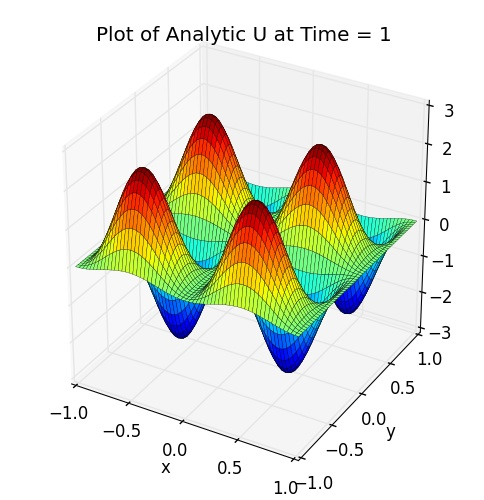
\includegraphics[width=2.5in]{C:/Users/HONGJI/Latex Home directory/Pm1a_pf2_U_exact_t_1_grid_60 - Copy.jpg}
		\caption{Analytic $U$ velocity at $t=1$}\label{fig:6.1a}		
	\end{subfigure}
	\quad
	\begin{subfigure}[t]{2.5in}
		\centering
		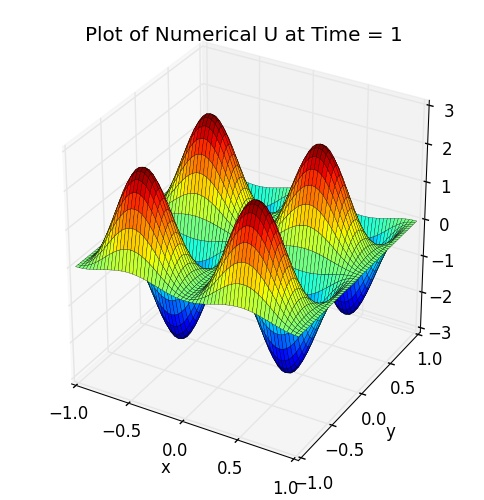
\includegraphics[width=2.5in]{C:/Users/HONGJI/Latex Home directory/Pm1a_pf2_uf_t_1_grid_60 - Copy.jpg}
		\caption{Numerical $U$ velocity at $t=1$}\label{fig:6.1b}
	\end{subfigure}
	\quad
	\begin{subfigure}[t]{2.5in}
		\centering
		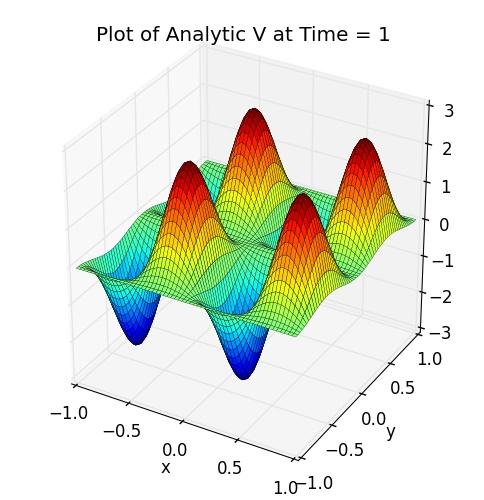
\includegraphics[width=2.5in]{C:/Users/HONGJI/Latex Home directory/Pm1a_pf2_V_exact_t_1_grid_60 - Copy.jpg}
		\caption{Analytic $V$ velocity at $t=\pi$}\label{fig:6.1c}
	\end{subfigure}
	\quad
	\begin{subfigure}[t]{2.5in}
		\centering
		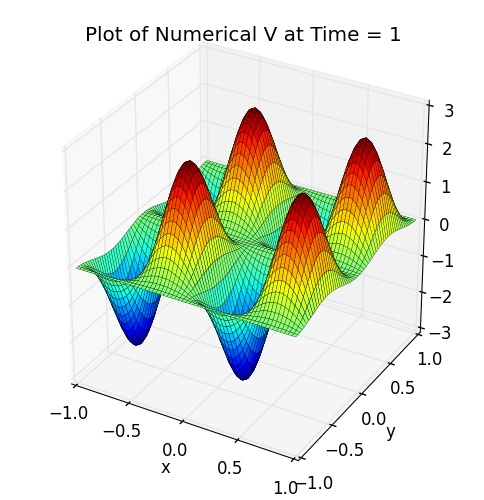
\includegraphics[width=2.5in]{C:/Users/HONGJI/Latex Home directory/Pm1a_pf2_vf_t_1_grid_60 - Copy.jpg}
		\caption{Numerical $V$ velocity at $t=\pi$}\label{fig:6.1d}
	\end{subfigure}
	\quad	
	\begin{subfigure}[t]{2.5in}
		\centering
		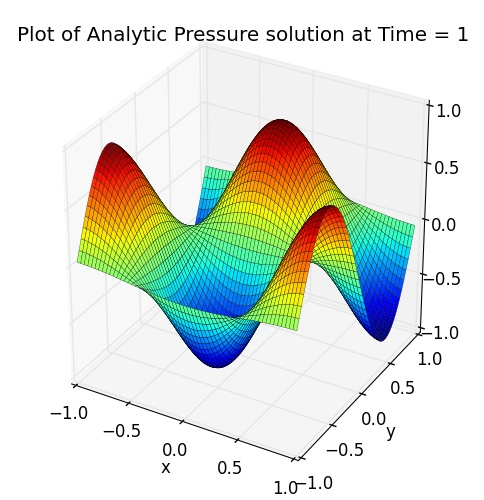
\includegraphics[width=2.5in]{C:/Users/HONGJI/Latex Home directory/Pm1a_pf2_P_exact_t_1_grid_60 - Copy.jpg}
		\caption{Analytic pressure ($P$) at $t=3.14$}\label{fig:6.1e}
	\end{subfigure}
	\quad	
	\begin{subfigure}[t]{2.5in}
		\centering
		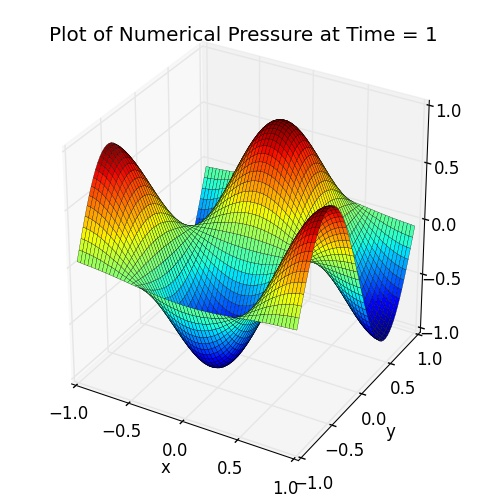
\includegraphics[width=2.5in]{C:/Users/HONGJI/Latex Home directory/Pm1a_pf2_pf_t_1_grid_60 - Copy.jpg}
		\caption{Numerical pressure ($P$) at $t=3.14$}\label{fig:6.1f}
	\end{subfigure}
	\caption{Plot of exact solutions ($U,V,P$) at time $t=1$ on the spatial domain of $[-1,1]^2$ with grid size $60 \times 60$ and $CFL=0.5$}\label{fig:6.1}
\end{figure}

The Log-Log plot for errors in velocity and pressure are summarised below. We have run the code from $15 \times 15$ up to the $480 \times 480$ the finest. Even finer grids are also able to be calculated by increasing the number of cells, but this is omitted due to the exceedingly long hours take in solving the Poisson equations. (\textbf{will add the velocity convergence plots soon} Due to limited space, only Pressure convergence errors are presented here as it is more important. (\textbf{should I include all plots including velocities in Appendix?})\\

Interestingly we observe an outlier at grid size 15 where the pressure error is very large compared to the those at the finer grids. This is observed in all methods for this test problem. This is most likely due to the large spatial error which dominates at such a small grid size. Hence for the sake of reliability, we excluded these data points when computing the convergence rates. The errors after grid 60 reduces consistently and converge asymptotically to the second order reference slope (especially for $Pm\,2$ and Gauge method). This asymptotic convergence behaviour is due to the gradual phasing out of spatial errors dominance at finer and finer grids. This is the most common error behaviour in Projection methods and our results now fully line up with those found in literature. \\

Even though $Pm\,2$ and Gauge methods show optimal 2nd order convergence for this test problem, the projection method $Pm\,1\,(b)$ however shows deprecated convergence especially measured in $L_\infty$. The reduced accuracy in $L_\infty$ implies the presence of numerical boundary layer and this is confirmed by the Pressure error field plot shown in Figure. The $3D$ surface plot of Pressure error field is almost identical to that of the non-normalised counterpart but at a much reduced magnitude. This indicates that our $\phi$ correction is working. \\

The Plots of divergence of intermediate velocity fields for $Pm\,1\,(b)$ and $Pm\,2$ are similar in shape but differ by magnitude. In fact the numerical boundary layer is much more pronounced in $Pm\,2$ than than of$Pm\,1\,(b)$. This makes the convergence rate for $\nabla \cdot \textbf{u}^*$ for $Pm\,2$ much degraded (from 0.5 order in $L_\infty$ to first order in $L_1$) compared to that of $Pm\,1\,(b)$ (from first order in $L_\infty$ to 1.8 order for $L_1$). It is however surprising to see that the Pressure convergence rate is better for $Pm\,2$. We infer that this is due to the better boundary condition used for the projection step where second order approximation to $\phi^{n+1}$ was used in $Pm\,2$. Even though our normal mode analysis has predicated that $Pm\,1\,(b)$ with the boundary condition of $\textbf{u}^*|_{\partial \Omega} = \textbf{u}^{n+1}|_{\partial \Omega}$ for projection should be second order accurate too, the numerical results show the contrary. The exact cause of this non-smoothness in pressure at the corners of the domain is rather still unknown. Suggested by Shen that this is caused by non-smoothness of domain. However this could not explain why $Pm\,2$ and Gauge method display optimal convergence in the same domain. The spikes in pressure error field is amplified in the plot of divergence of intermediate velocity field where large numerical boundary appears. It seems like the boundary layer gets thick rapidly when approaching boundaries. This implies large change in pressure gradients along boundary. We infer that this might be due to how the spatial interpolation is done in a staggered grid where ``ghost cell" are required in order to calculate the pressure gradients along boundary. We have used cubic interpolation to do this and it could lead to large ghost cell values. and hence causing large pressure normal gradients.\\

This large numerical boundary layer problem could be reduced by making velocity variables to satisfy a ``free boundary condition" where its third order derivative is zero. This was suggested by Brown in \cite{brown2001accurate}. However this is problem dependent and due to limited space and time we did not implement this.\\



\begin{figure}[H]
	\centering
	\begin{subfigure}[t]{4.5in}
		\centering
		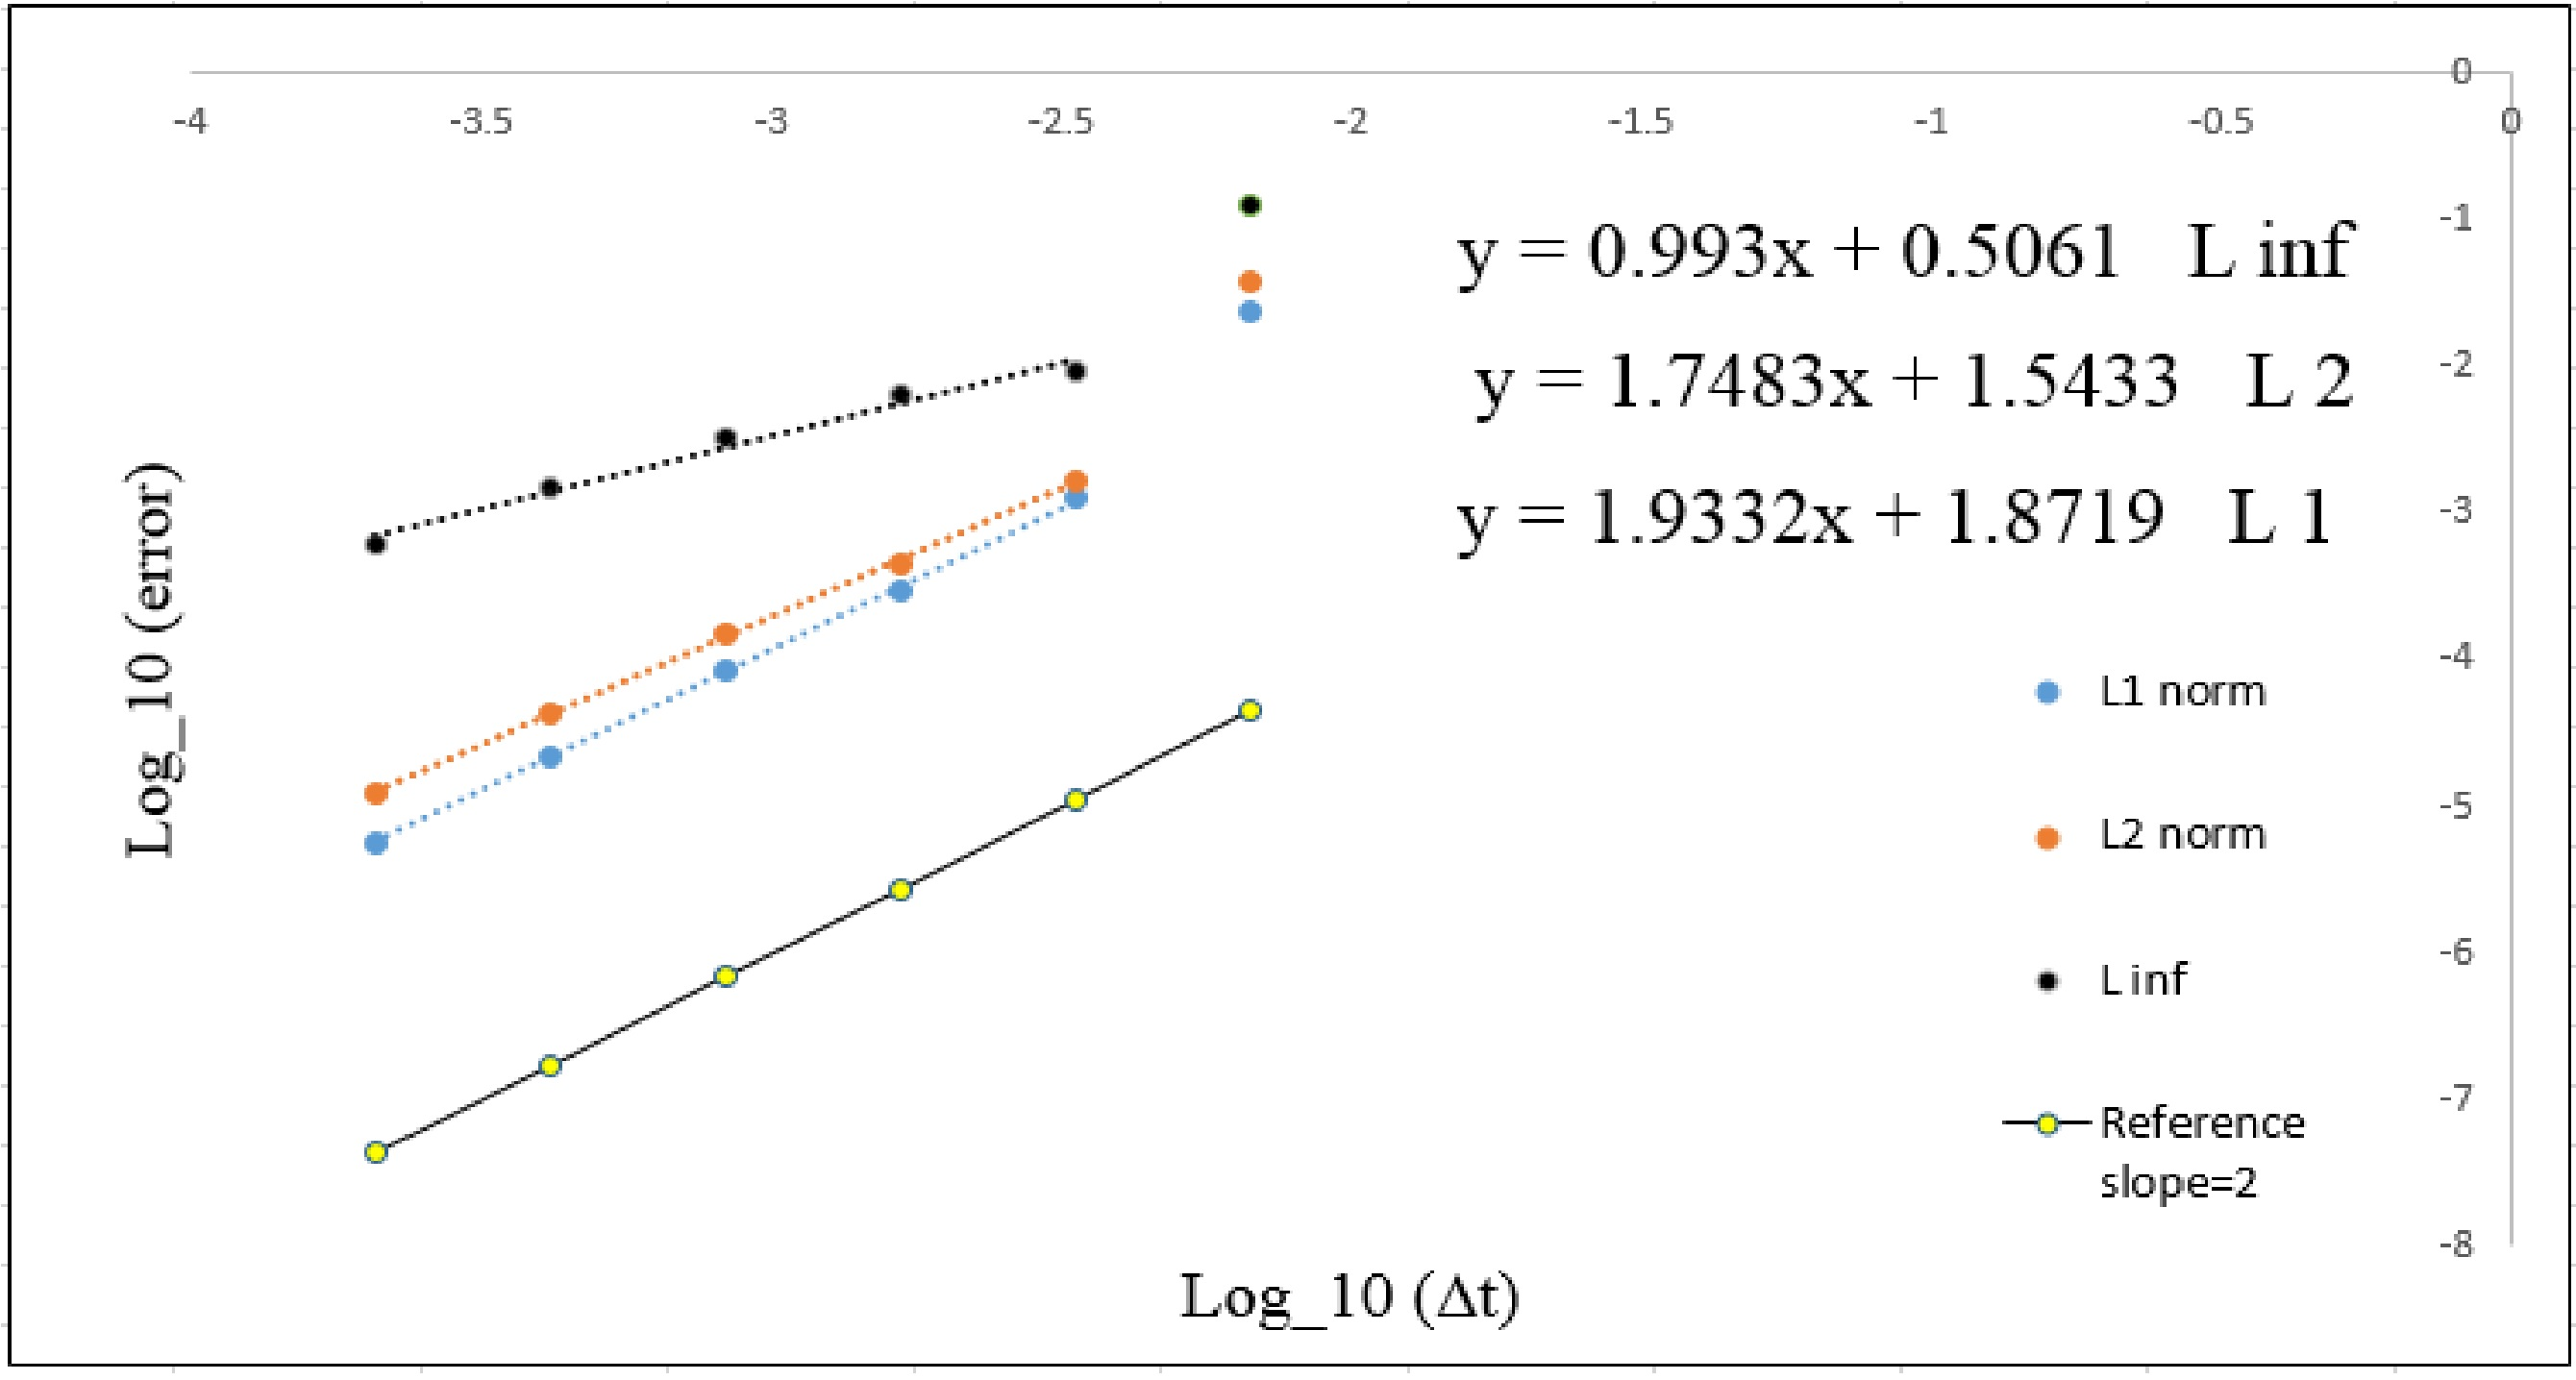
\includegraphics[width=4.5in]{C:/Users/HONGJI/Latex Home directory/Pm1b_pf2_np_P_rate_c_0_5.jpg}
		\caption{Log-Log plot of Convergence rate for Pressure}\label{fig:6.19a}		
	\end{subfigure}
	\quad
	\begin{subfigure}[t]{4.5in}
		\centering
		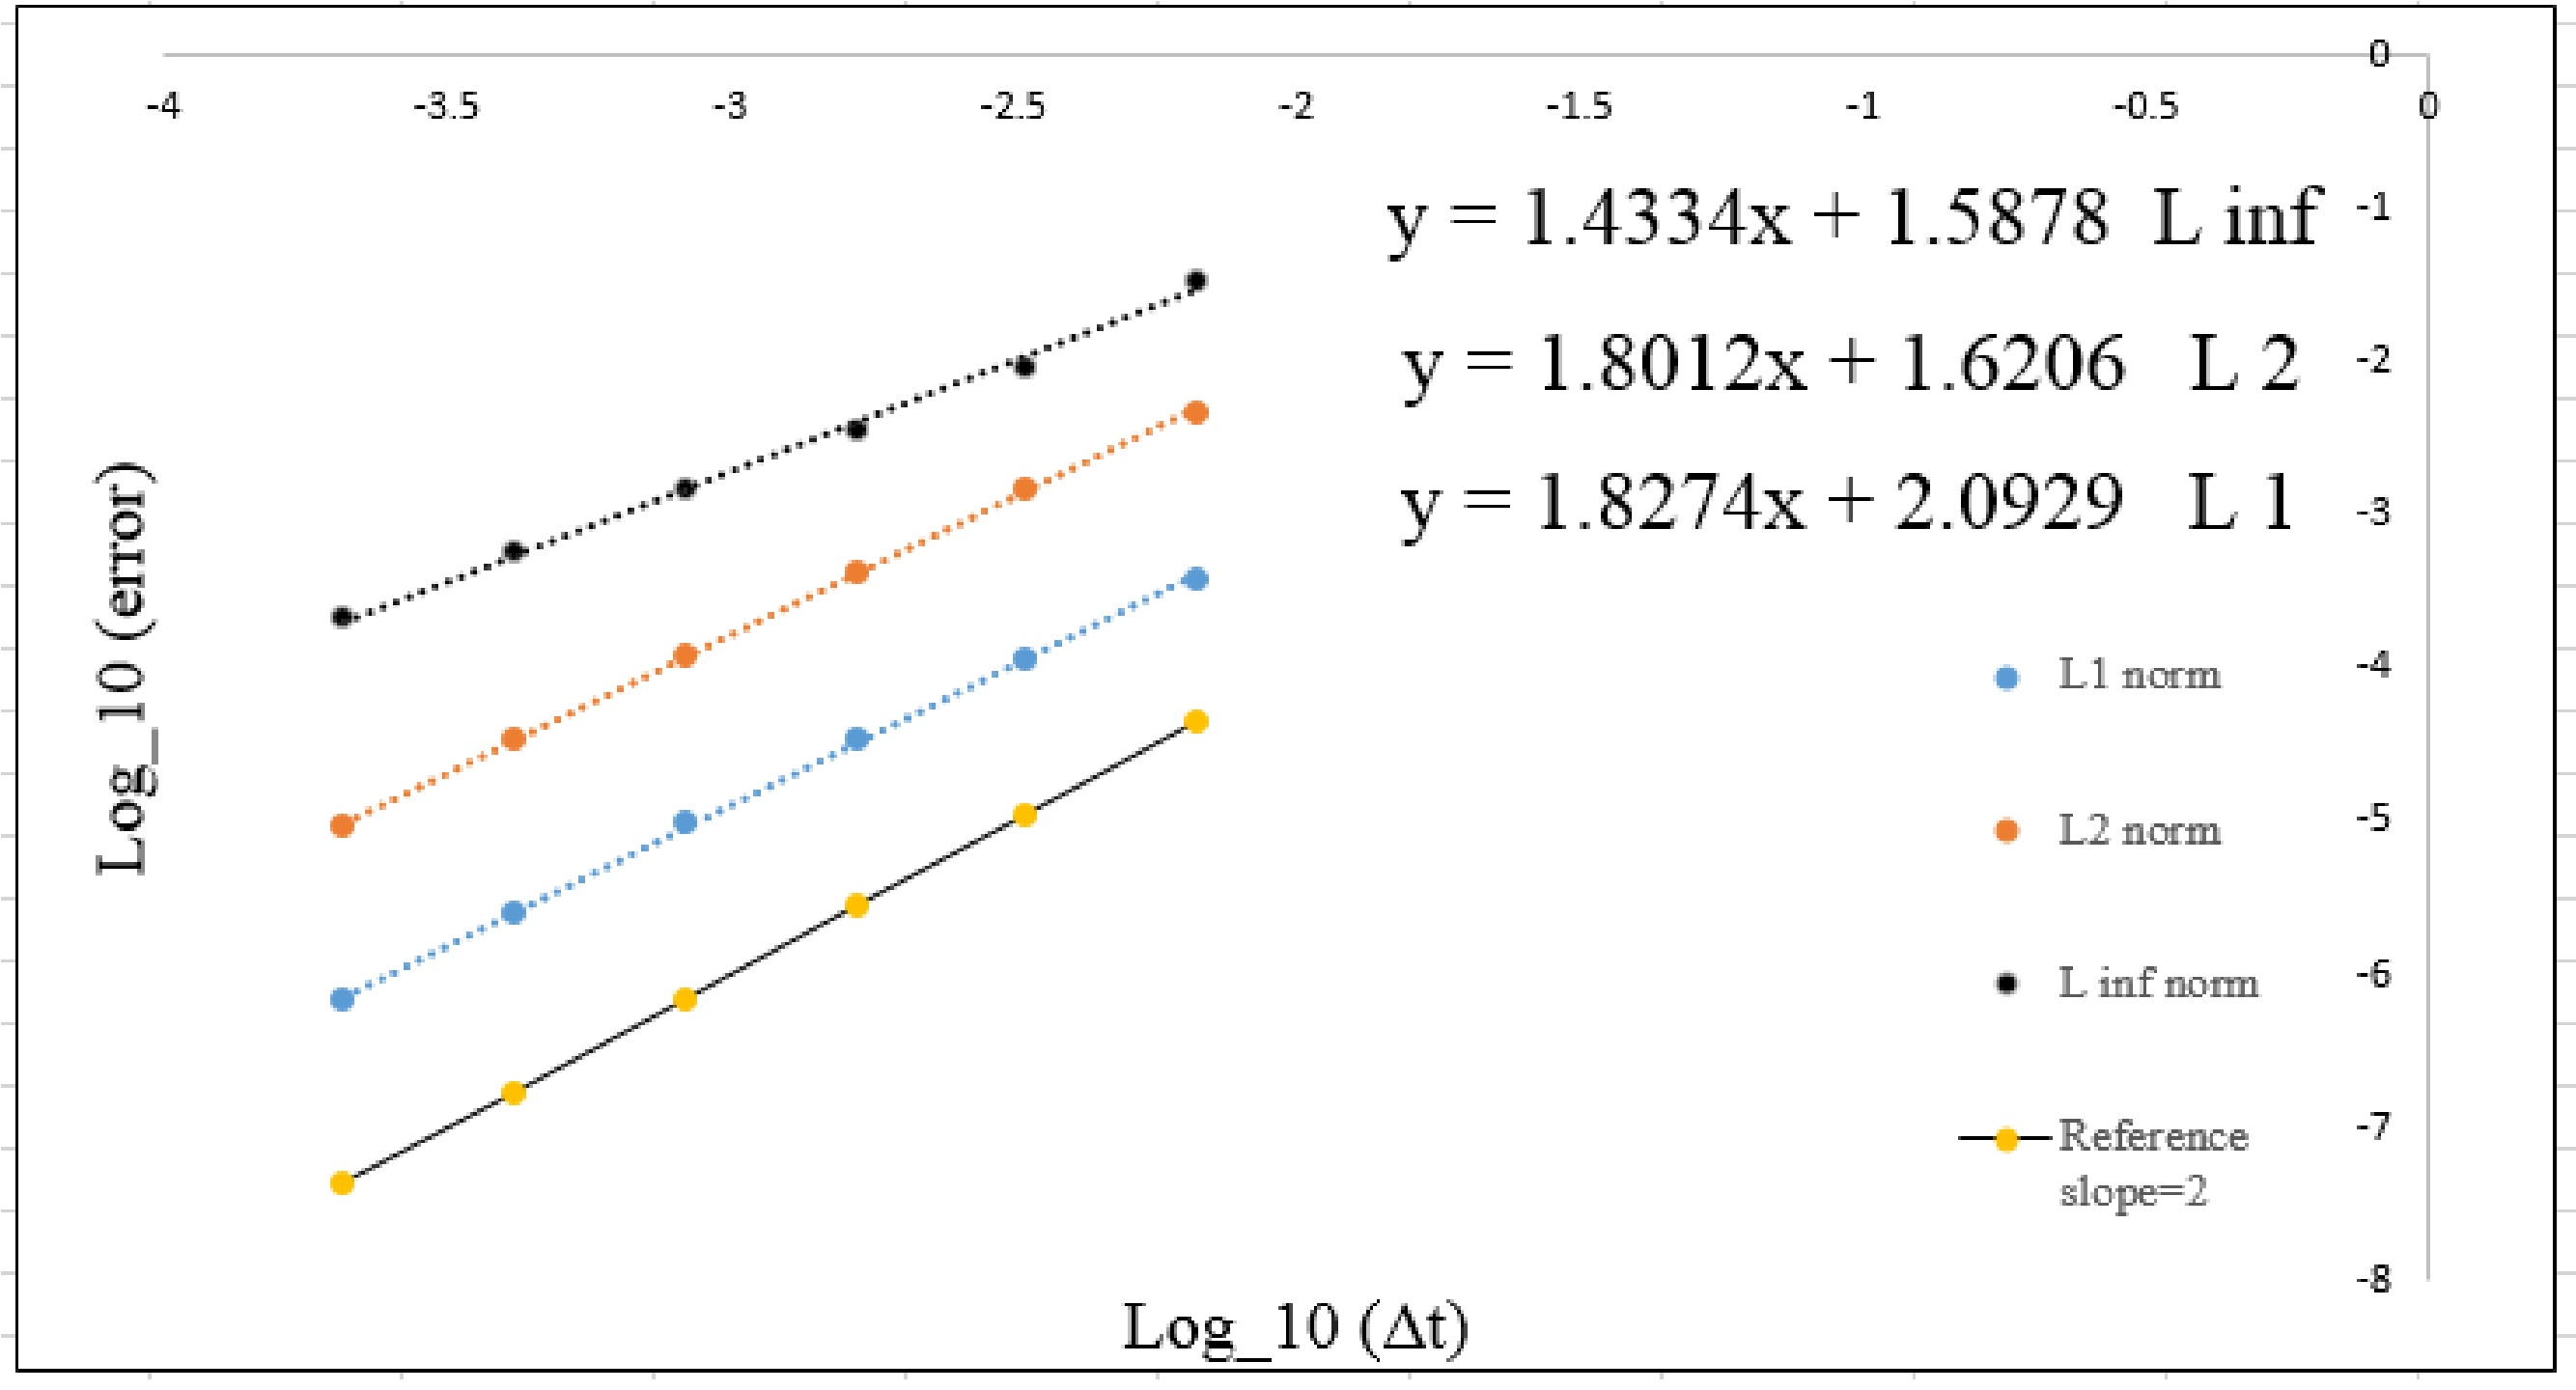
\includegraphics[width=4.5in]{C:/Users/HONGJI/Latex Home directory/Pm1b_pf2_np_div_uv_rate_c_0_5.jpg}
		\caption{Log-Log plot of Convergence rate for $\nabla \cdot \textbf{u}^*$. }\label{fig:6.19b}
	\end{subfigure}
	\caption{Plot of Convergence rates for $Pm\,1\,(b)$ with Normalised Pressure approach used. Domain: $[-1,1]^2$, time = 1 and CFL = 0.5. In each plot, the data points corresponding to grid sizes of 15, 30, 60, 120, 240, and 480. Subplot (b) shows the error in the divergence of intermediate velocity. The data points between different norms are close to each. Hence $L_1$ and $L_\infty$ norms were shifted up and down by 0.5 respectively to distinguish from $L_2$ norm data points.}\label{fig:6.16}
\end{figure}

\begin{figure}[H]
	\centering
	\begin{subfigure}[t]{4.5in}
		\centering
		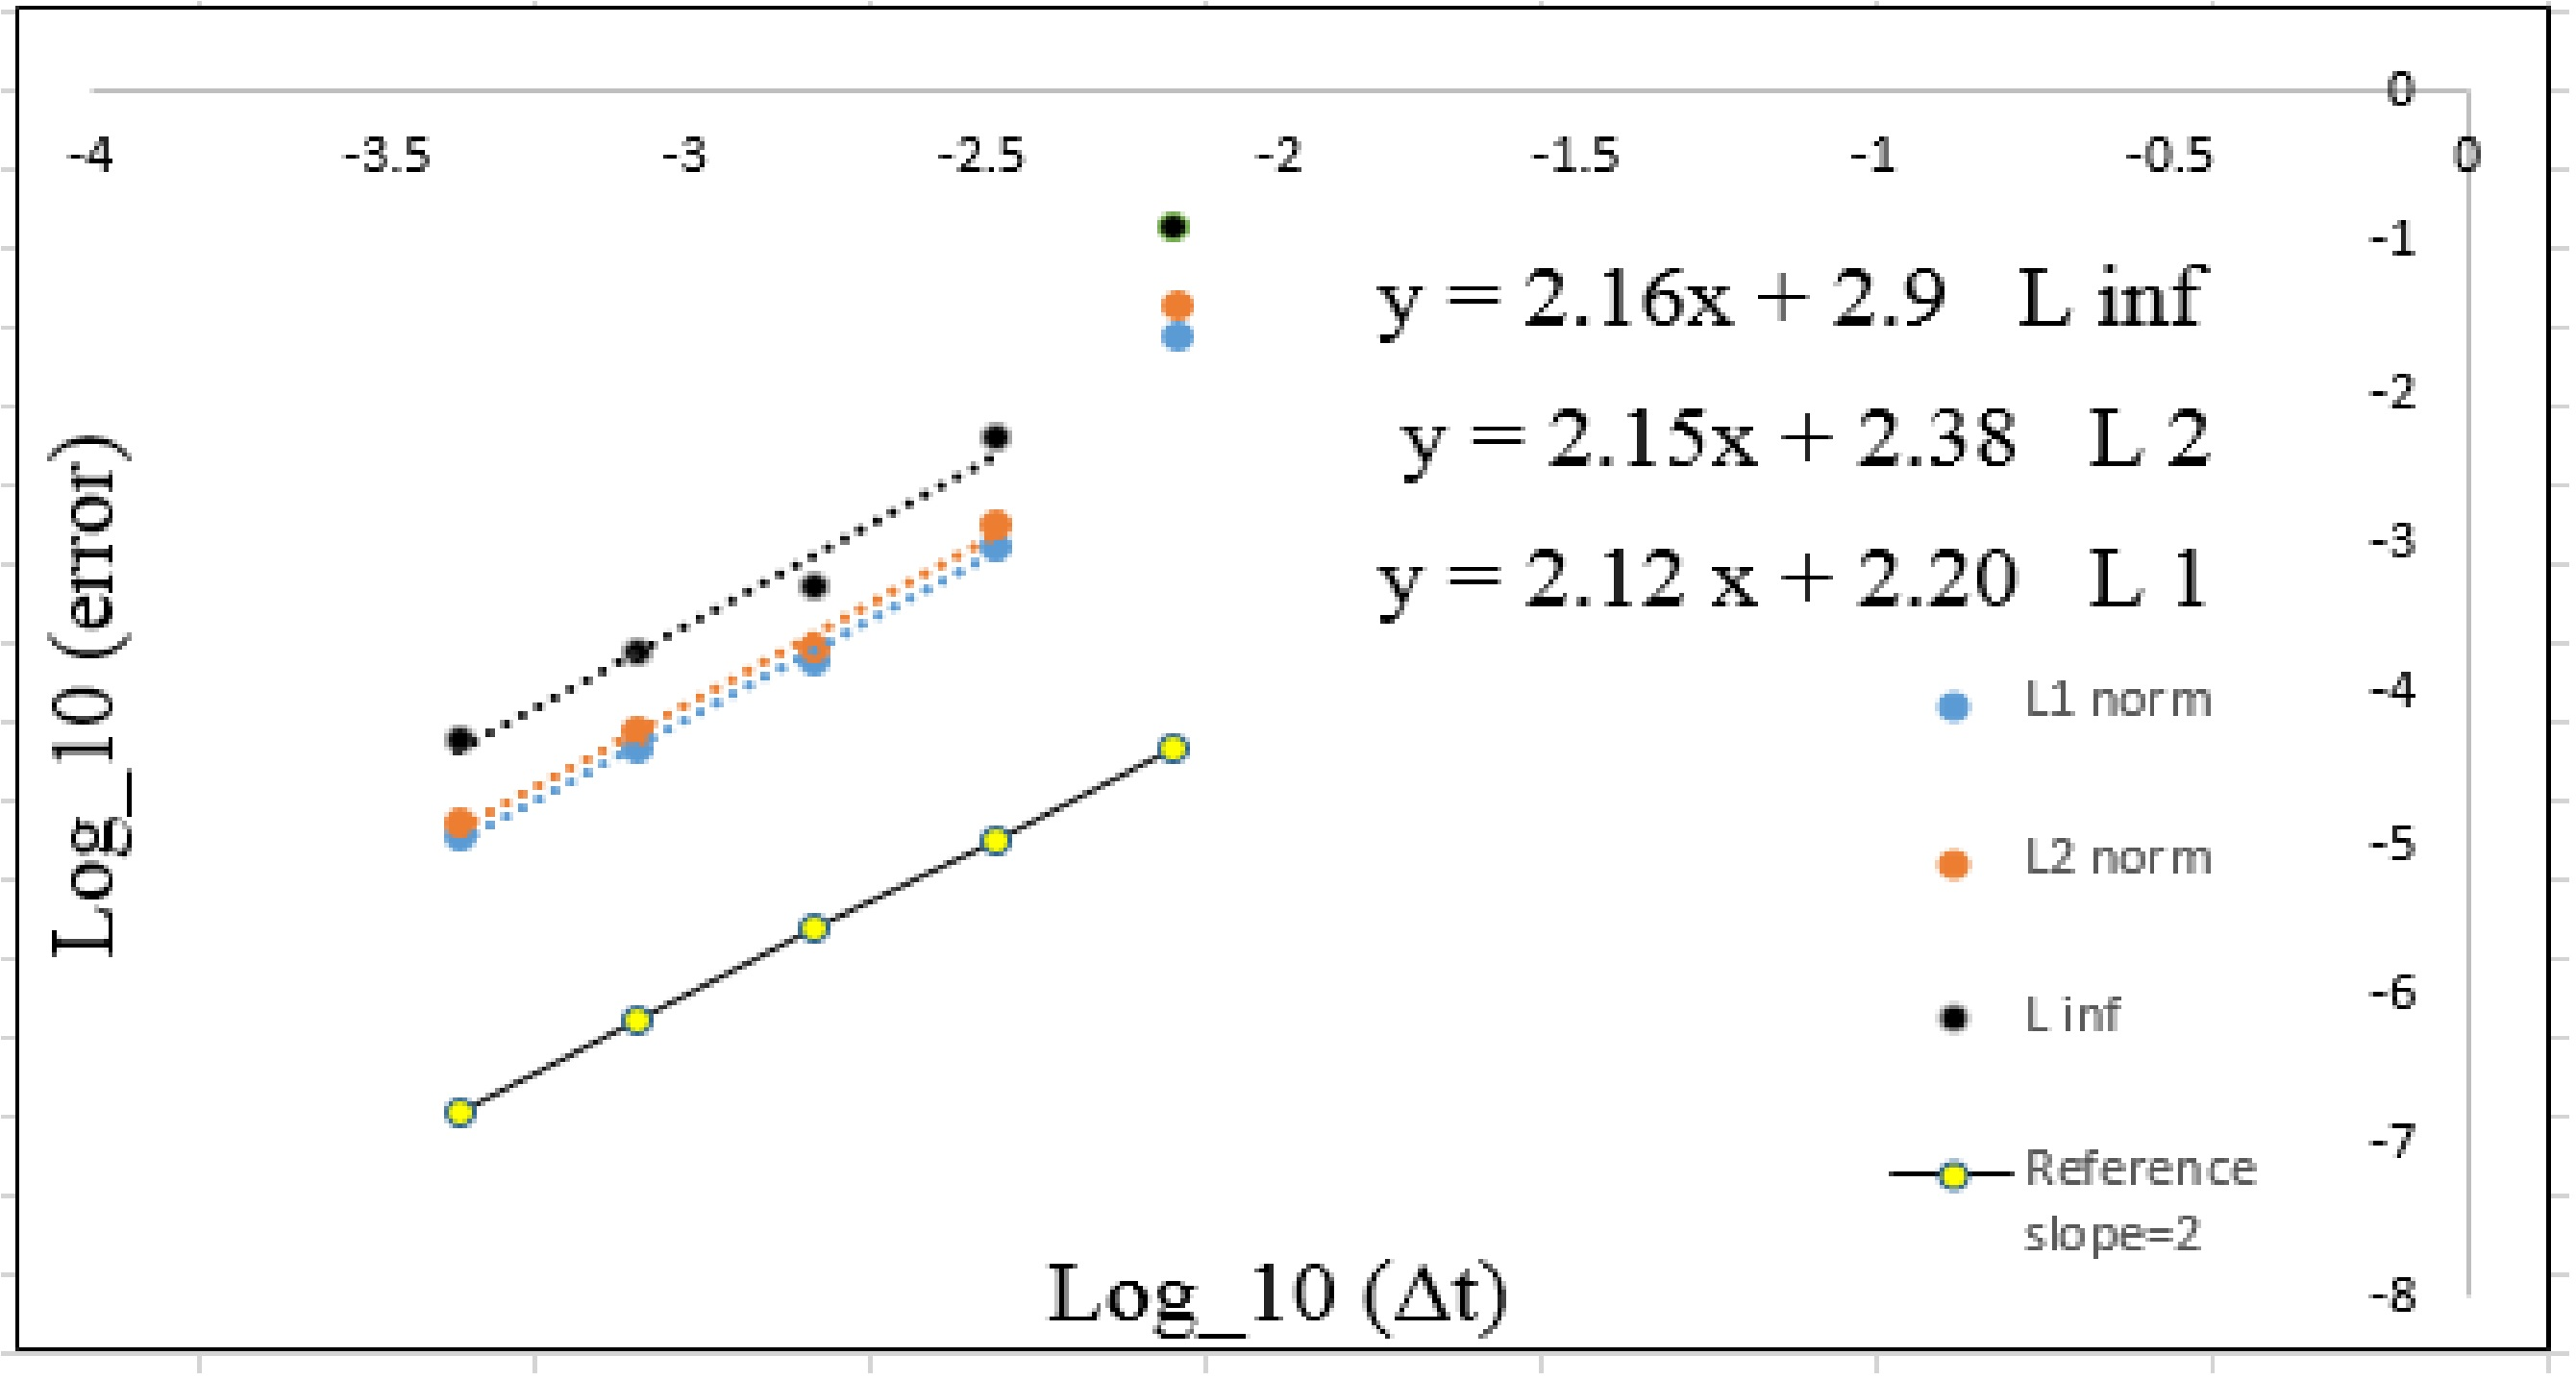
\includegraphics[width=4.5in]{C:/Users/HONGJI/Latex Home directory/Pm2_pf2_np_P_rate_c_0_5.jpg}
		\caption{Log-Log plot of Convergence rate for Pressure}\label{fig:6.19a}		
	\end{subfigure}
	\quad
	\begin{subfigure}[t]{4.5in}
		\centering
		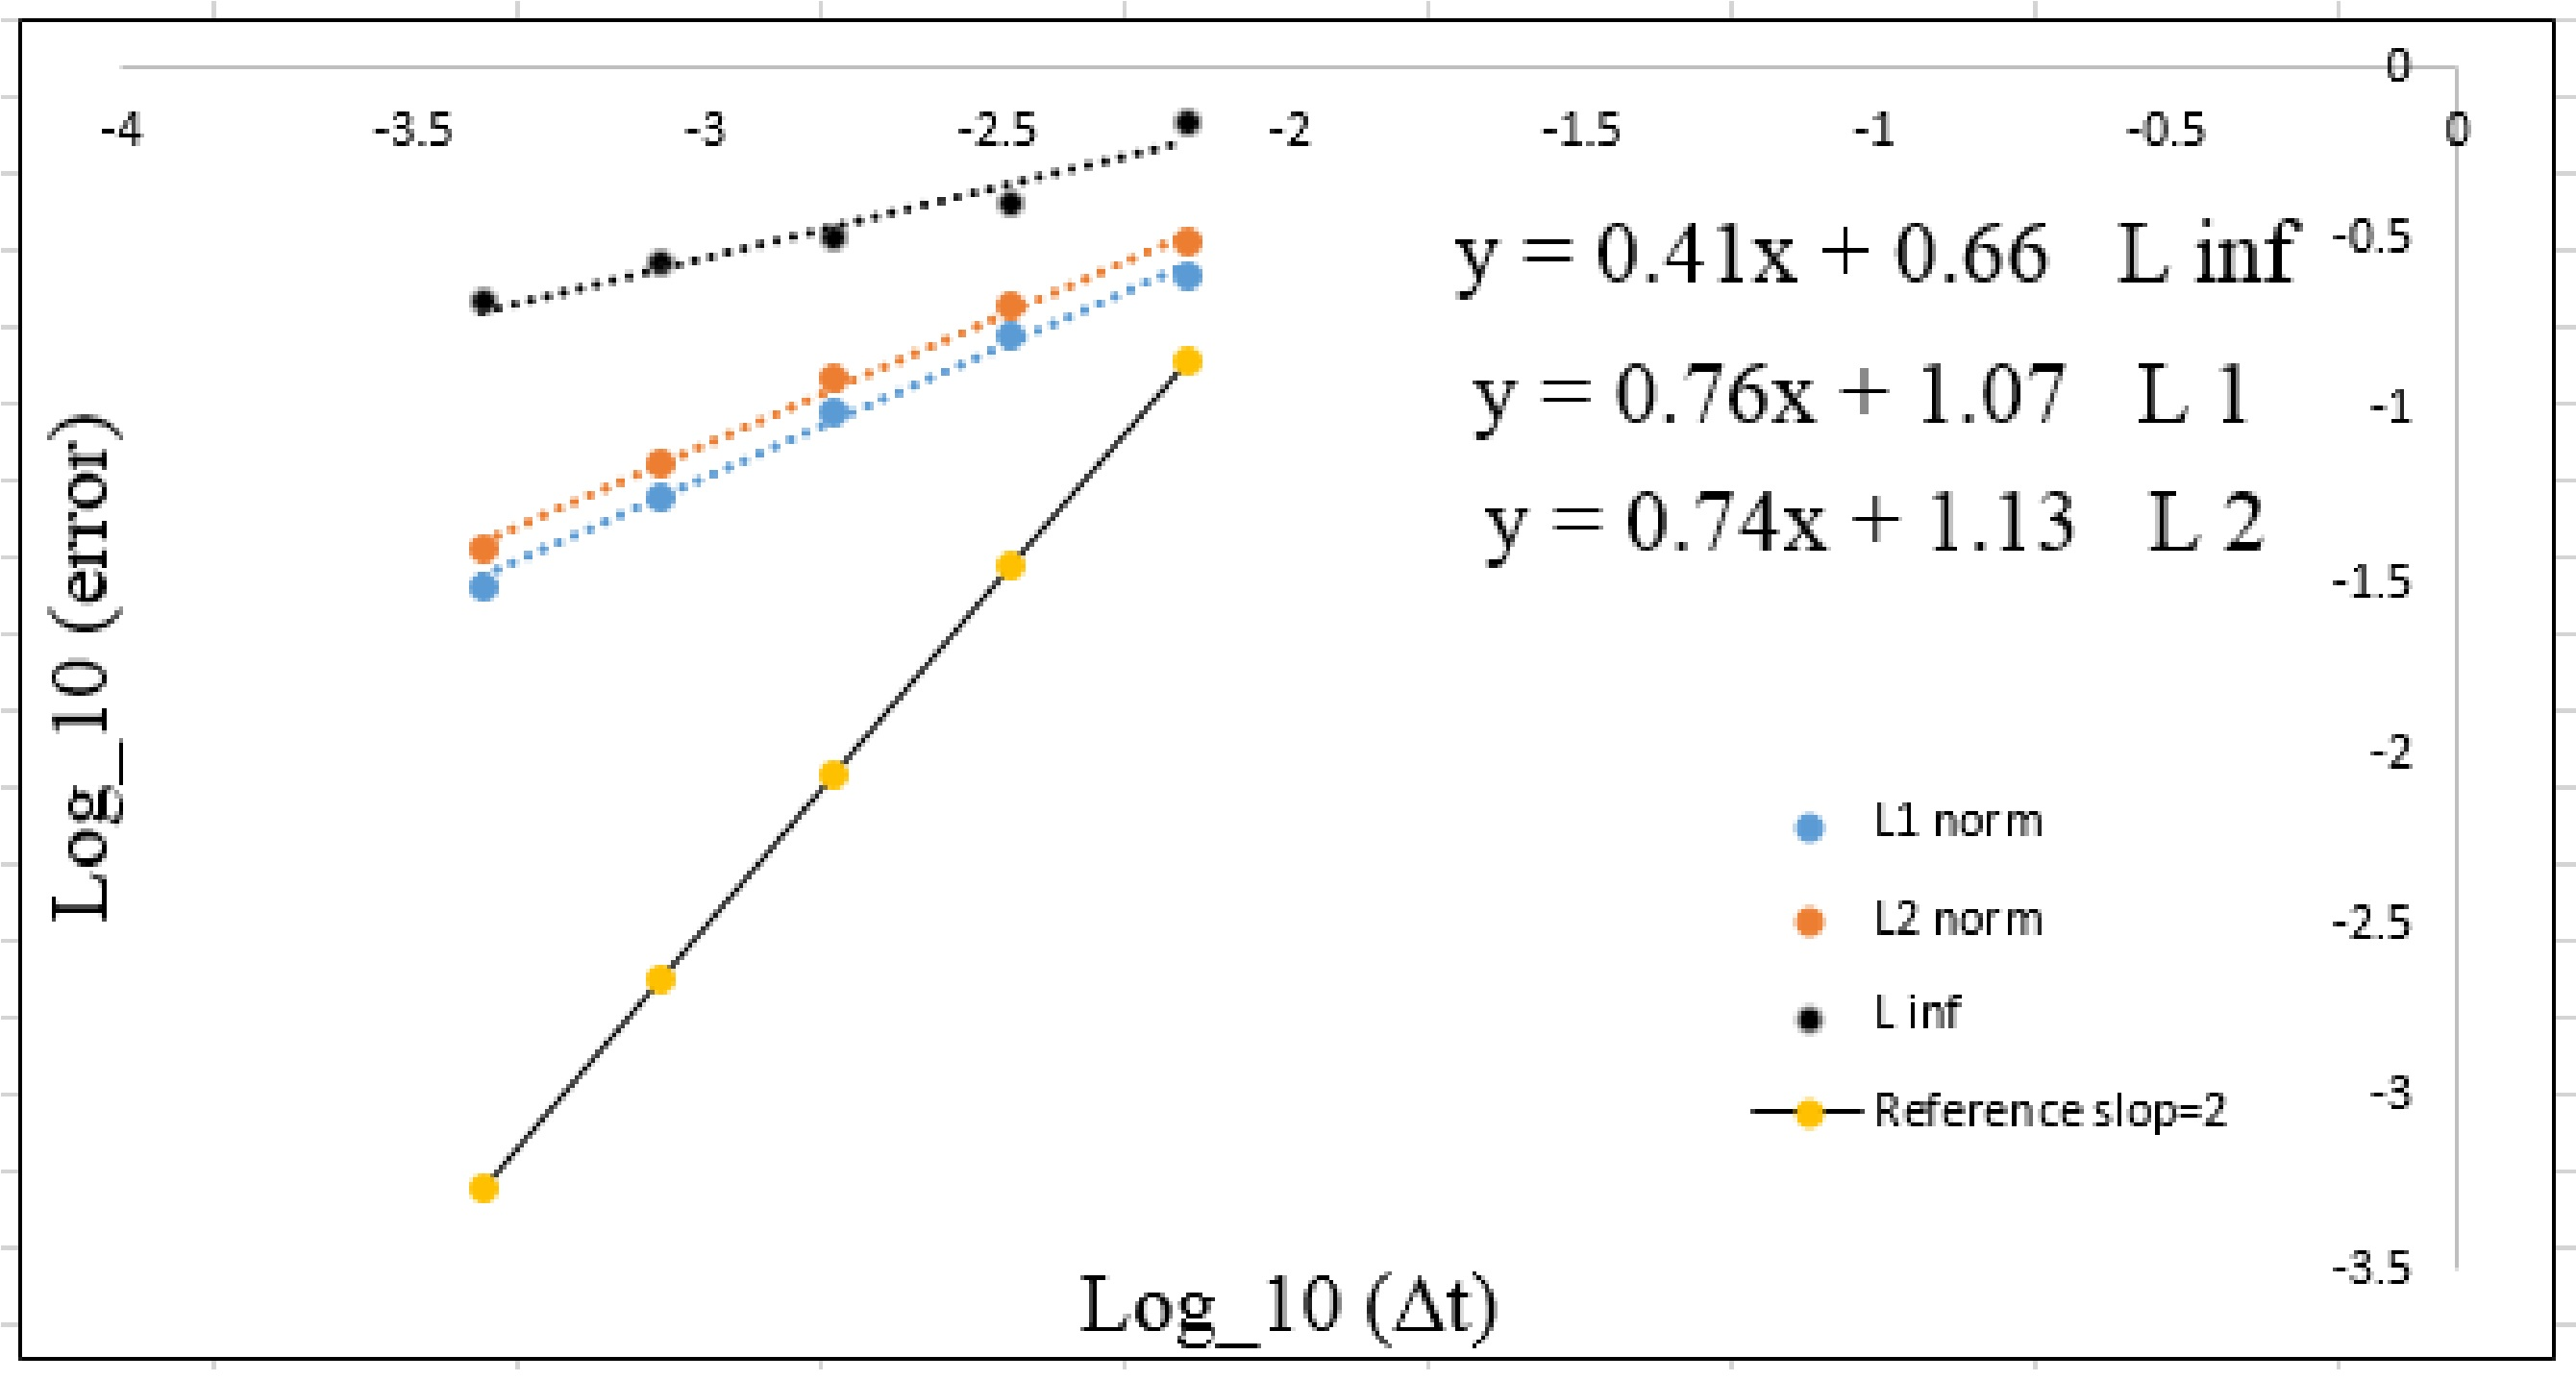
\includegraphics[width=4.5in]{C:/Users/HONGJI/Latex Home directory/Pm2_pf2_np_div_uvstar_rate_c_0_5.jpg}
		\caption{Log-Log plot of Convergence rate for $\nabla \cdot \textbf{u}^*$. }\label{fig:6.19b}
	\end{subfigure}
	\caption{Plot of Convergence rates for $Pm\,2$ with Normalised Pressure approach used. Domain: $[-1,1]^2$, time = 1 and CFL = 0.5. In each plot, the data points corresponding to grid sizes of 15, 30, 60, 120, 240.}\label{fig:6.16}
\end{figure}
\textbf{I will try to add the 480 grid plot too}

\begin{figure}[H]
	\centering
	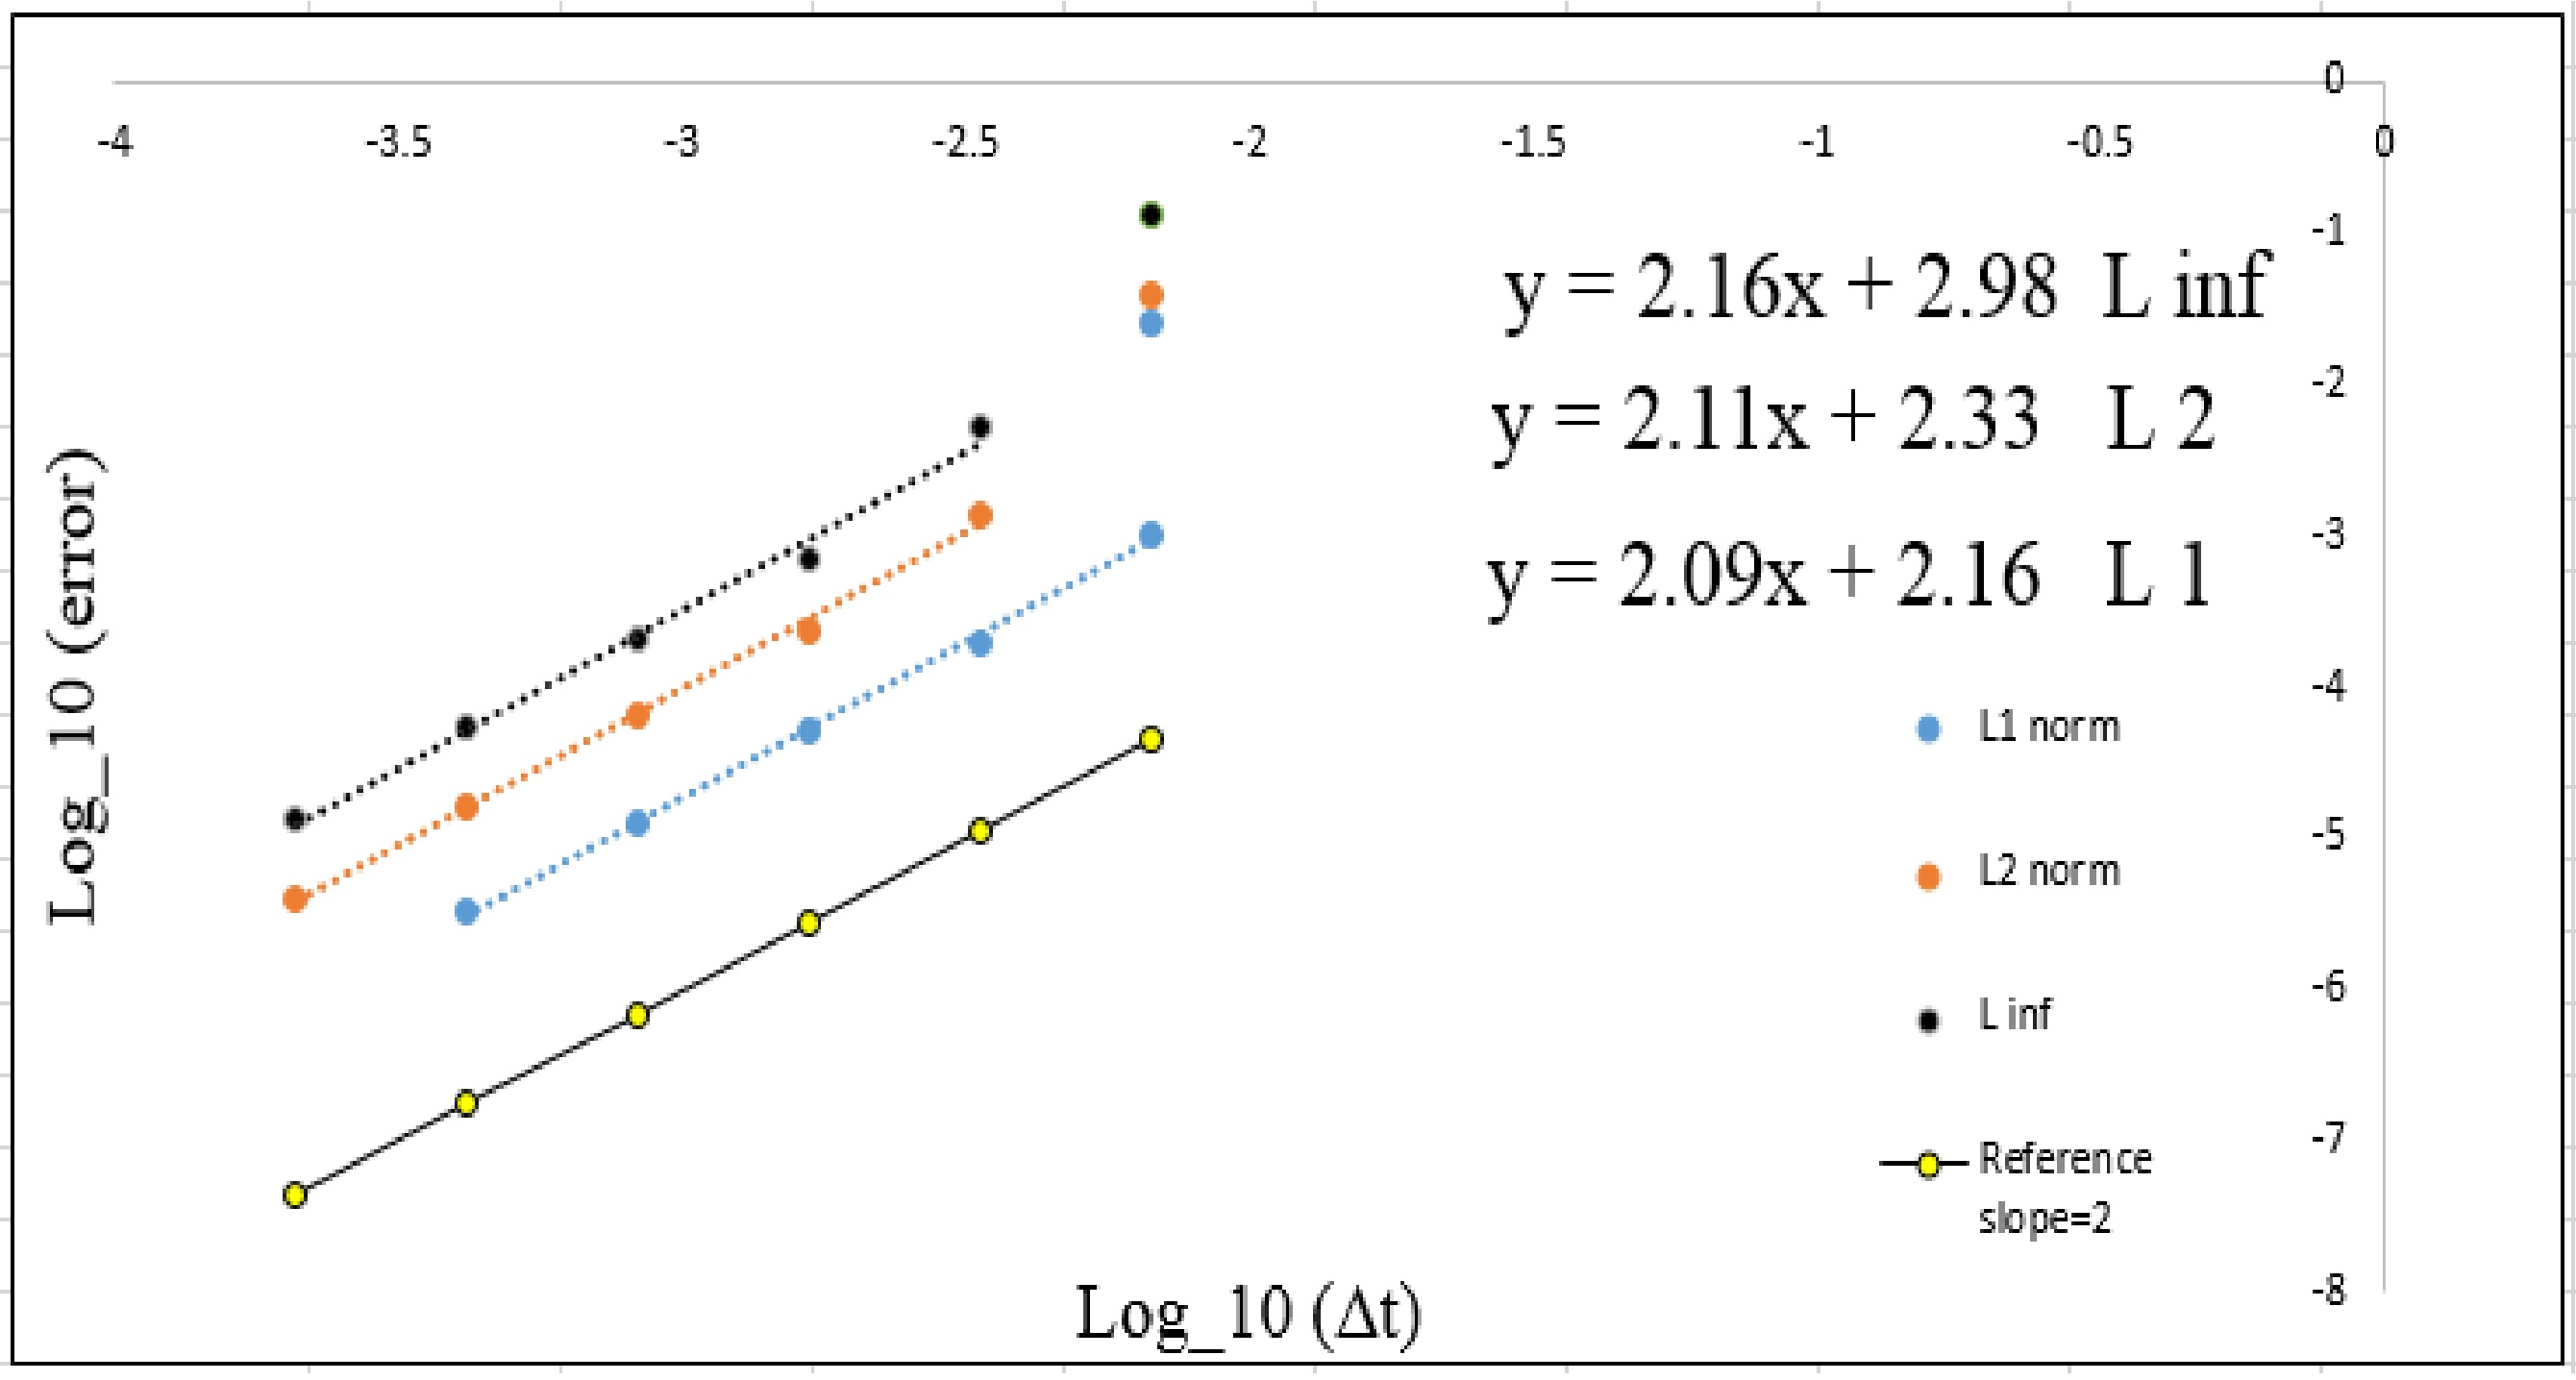
\includegraphics[width=4.5in]{C:/Users/HONGJI/Latex Home directory/Gauge_pf2_np_P_rate_c_0_5.jpg}
	\caption{Long-Log plot of Pressure Convergence rates for Gauge method with Normalised Pressure approach used. Domain: $[-1,1]^2$, time = 1 and CFL = 0.5. The data points corresponding to grid sizes of 15, 30, 60, 120, 240, and 480.}\label{fig:6.16}
\end{figure}

\begin{figure}[H]
	\centering
	\begin{subfigure}[t]{2.5in}
		\centering
		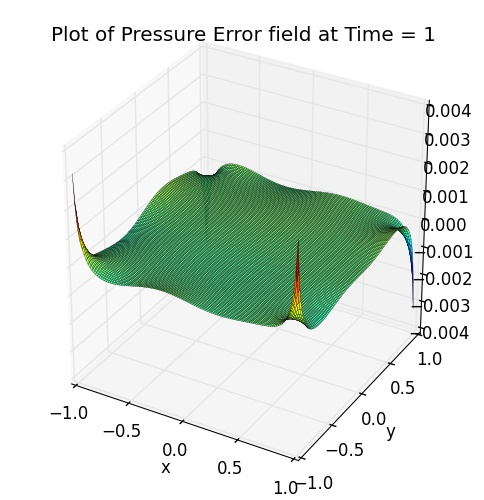
\includegraphics[width=2.5in]{C:/Users/HONGJI/Latex Home directory/Pm1b_pf2_np_P_error_t_1_grid_120.jpg}
		\caption{Pressure error field for $Pm\,1\,(b)$ method}\label{fig:6.19a}		
	\end{subfigure}
	\quad
	\begin{subfigure}[t]{2.6in}
		\centering
		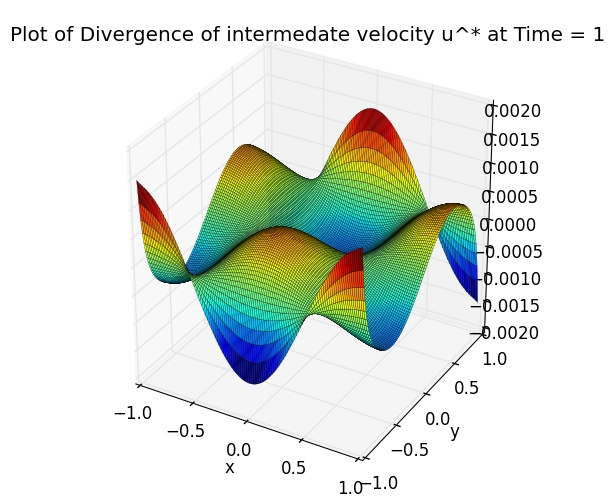
\includegraphics[width=2.6in]{C:/Users/HONGJI/Latex Home directory/Pm1b_pf2_np_div_uvstar_t_1_grid_120.jpg}
		\caption{Divergence of intermediate velocity field for $Pm\,1\,(b)$ method. }\label{fig:6.19b}
	\end{subfigure}
	\quad
	\centering
	\begin{subfigure}[t]{2.5in}
		\centering
		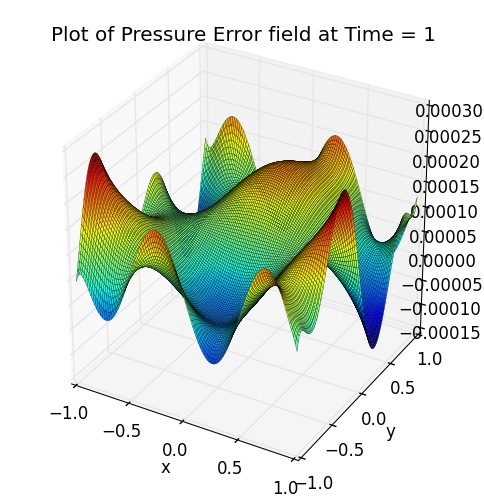
\includegraphics[width=2.5in]{C:/Users/HONGJI/Latex Home directory/Pm2_pf2_cN_np_P_error_t_1_grid_120.jpg}
		\caption{Pressure error field for $Pm\,2$ method}\label{fig:6.19c}		
	\end{subfigure}
	\quad
	\begin{subfigure}[t]{2.6in}
		\centering
		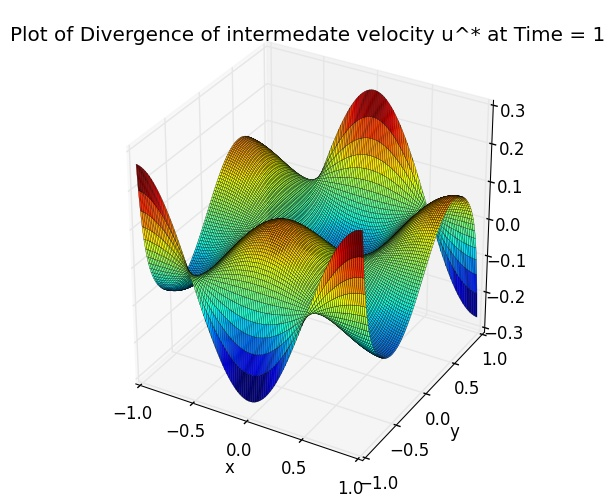
\includegraphics[width=2.6in]{C:/Users/HONGJI/Latex Home directory/Pm2_pf2_cN_np_div_uvstar_t_1_grid_120.jpg}
		\caption{Divergence of intermediate velocity field for $Pm\,2$ method.}\label{fig:6.19d}
	\end{subfigure}
	\quad
	\begin{subfigure}[t]{2.6in}
		\centering
		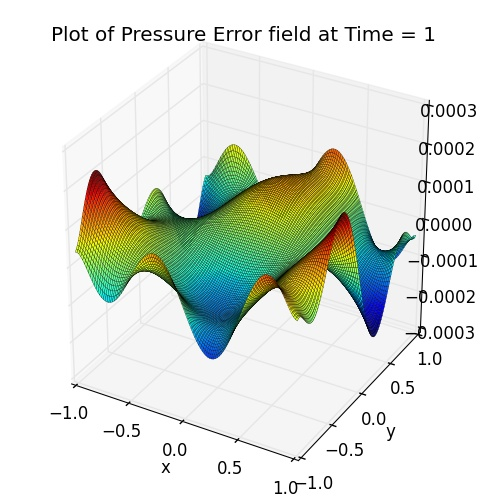
\includegraphics[width=2.6in]{C:/Users/HONGJI/Latex Home directory/Gauge_pf2_P_error_t_1_grid_120.jpg}
		\caption{Pressure error field for Gauge method. }\label{fig:6.19d}
	\end{subfigure}
	\caption{$3D$ surface plots of Pressure error fields and divergence of intermediate velocity (if applicable) for $Pm\,1\,(b)$, $Pm\,2$ and Gauge method (with Normalised Pressure approach used) at grid size of 120. Domain: $[-1,1]^2$, time = 1 and CFL = 0.5. }\label{fig:6.16}
\end{figure}

%_____________________
Next we have implemented a periodic boundary condition in y in order to mimic a periodic channel geometry.

\begin{itemize}
\item Periodic boundary
\end{itemize}
In addition, as the normal analysis based on periodic channel has predicated full second order accuracy in pressure for Projection methods, we infer that by imposing a periodic boundary condition on velocities would help to improve the convergence in pressure error. This helps to fix the lack of smooth of domain because this time the spatial interpolation error of ghost nodes next to boundaries are eliminated. The ghost nodes are now simply equal to the further most interior points at the opposite boundary. No interpolation is needed!\\

Now all the projection methods ($Pm\,1\,(b),\,Pm\,2$) restores second order accuracy. For $Pm\,1\,(b)$, the plot of divergence of intermediate velocity field and pressure error shows the numerical boundary layer disappears. This is consistent with our normal mode analysis. Hence our results has shown that Projection methods in particular $Pm\,1\,(b)$ with a lagged pressure approximation only shows second order accuracy in periodic channels. This findings was supported by the error analysis and numerical studies presented by Shen \cite{guermond2004error}. Now it is clear that the normal mode analysis is strongly dependent on the domain we work with and Projection methods are not fully 2nd order accurate in pressure in general domains. The reason that \emph{David} observed 2nd order convergence in pressure is most likely because they have analysed the schemes in a periodic channel \cite{brown2001accurate, guermond2006overview, guermond2004error}.

For spatial domain: $[-\dfrac{1}{2}, \dfrac{1}{2}]^2$
\begin{figure}[H]
	\centering
	\begin{subfigure}[t]{4.5in}
		\centering
		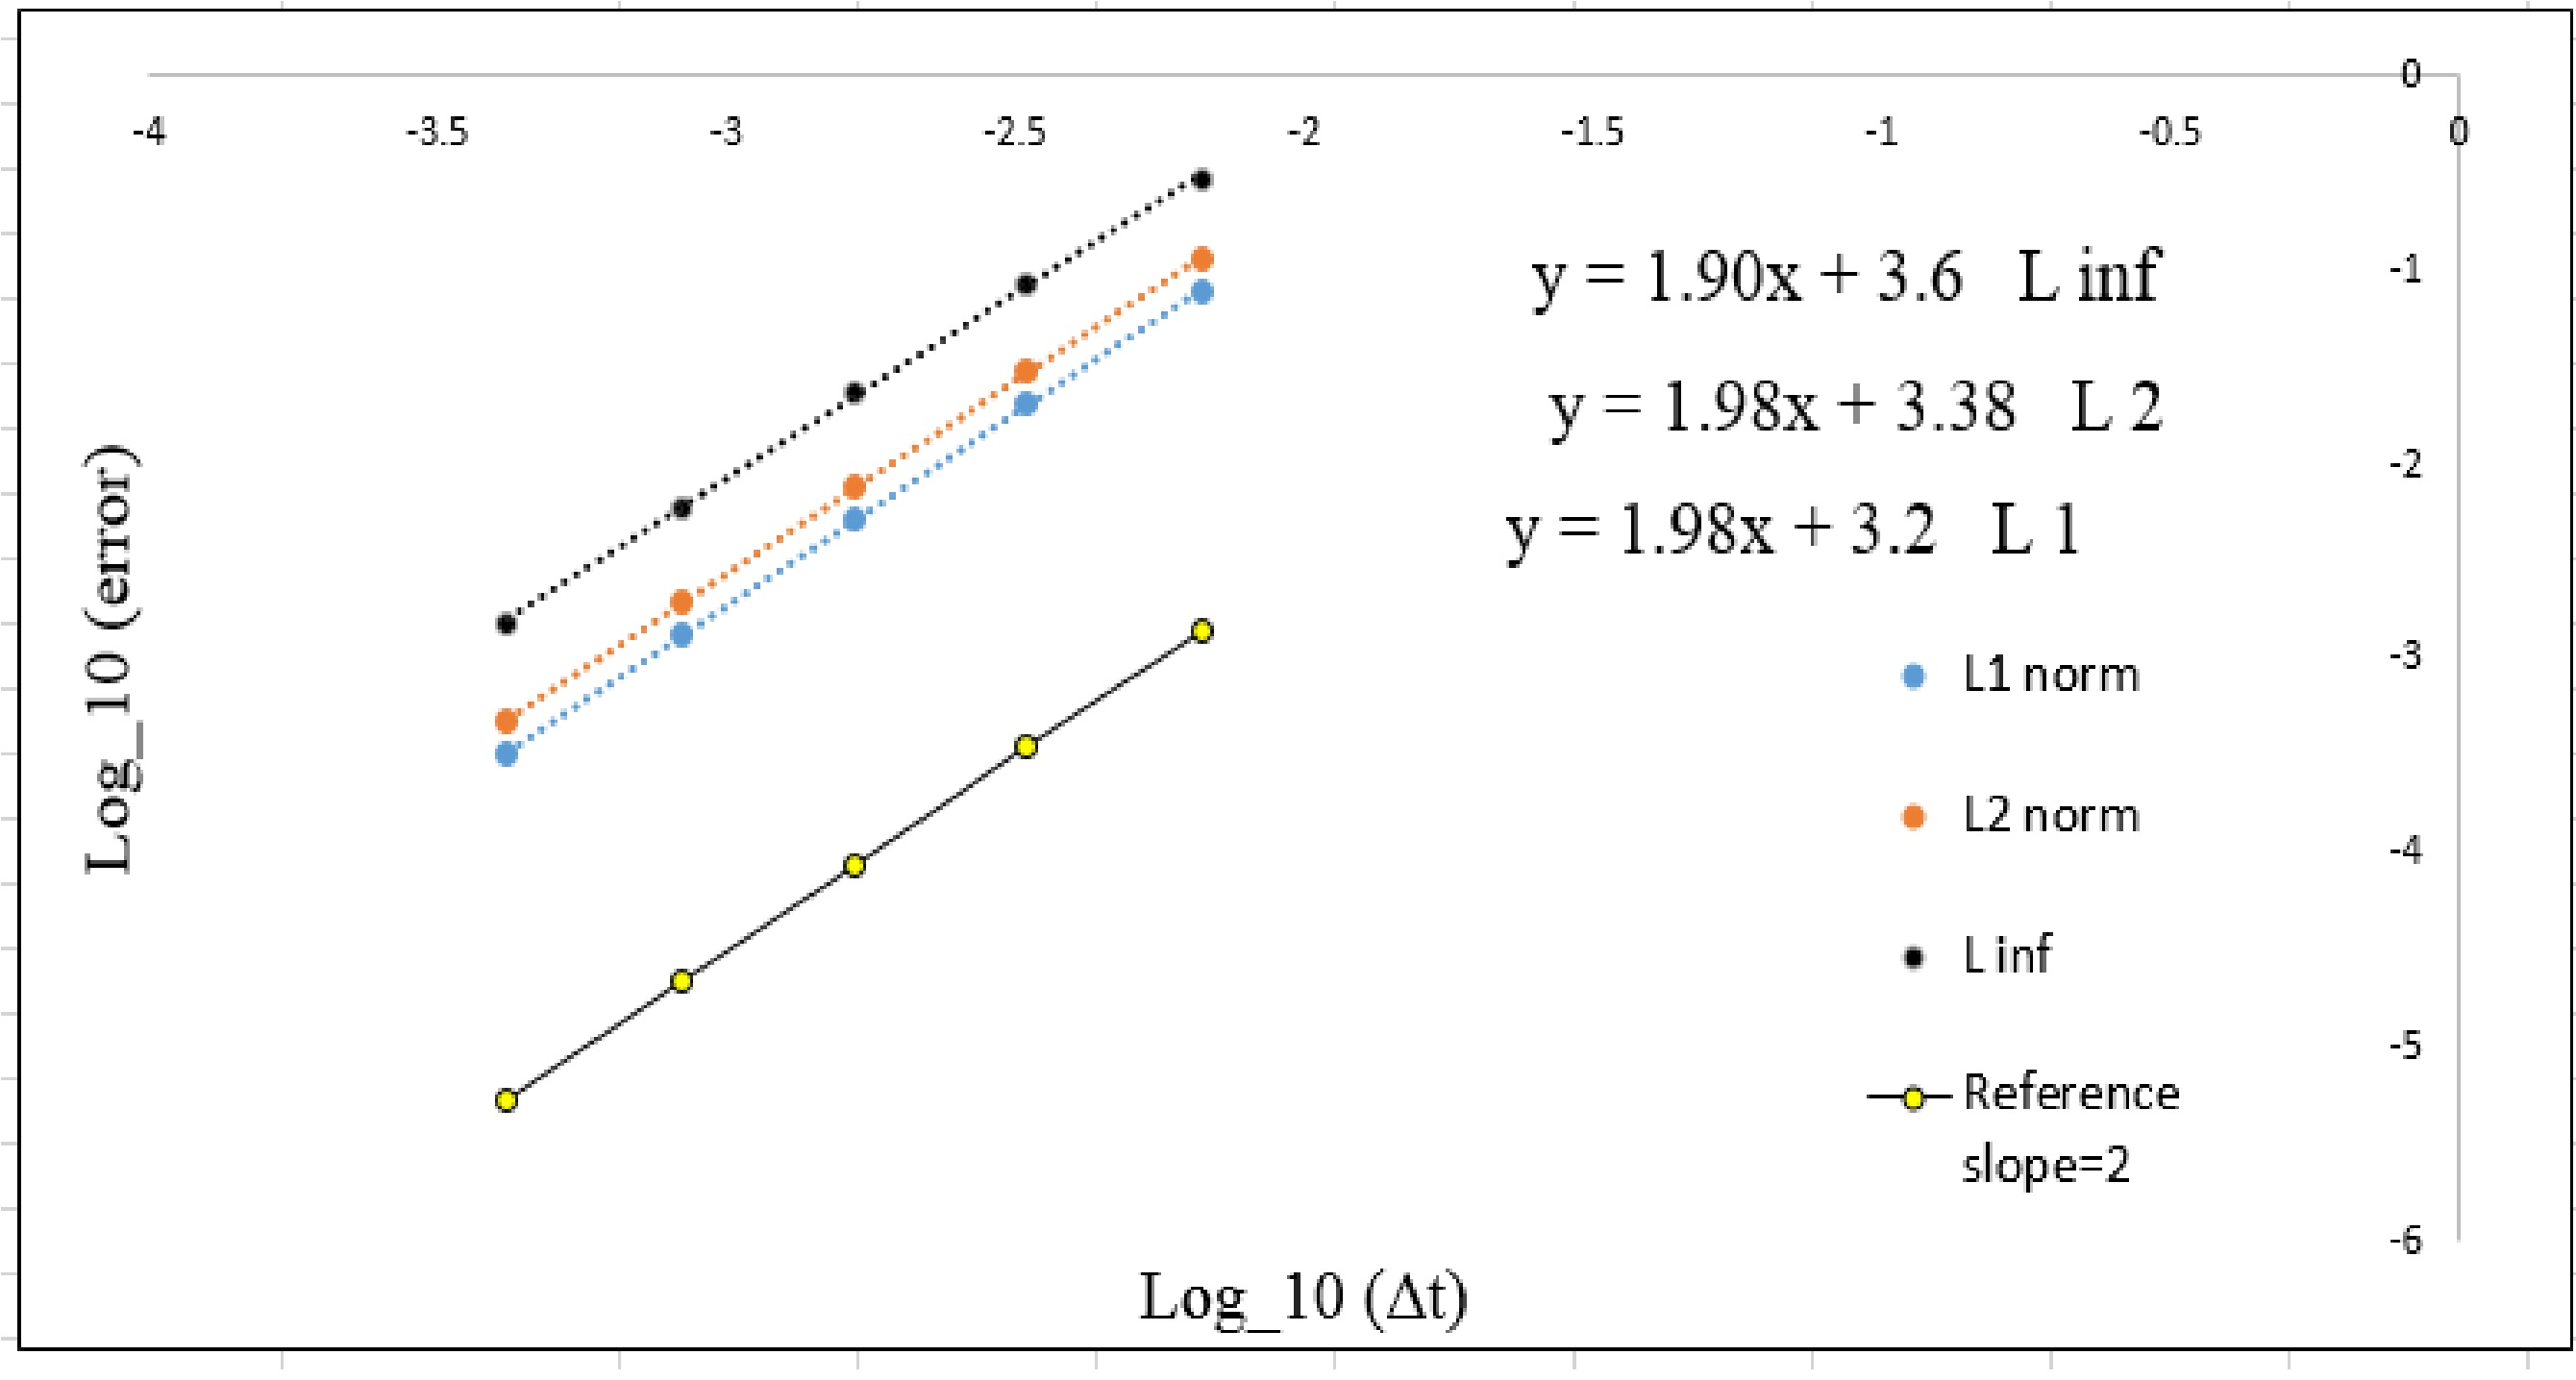
\includegraphics[width=4.5in]{C:/Users/HONGJI/Latex Home directory/Pm1b_pf2b_np_P_rate_c_0_5.jpg}
		\caption{Log-Log plot of Convergence rate for Pressure}\label{fig:6.19a}		
	\end{subfigure}
	\quad
	\begin{subfigure}[t]{4.5in}
		\centering
		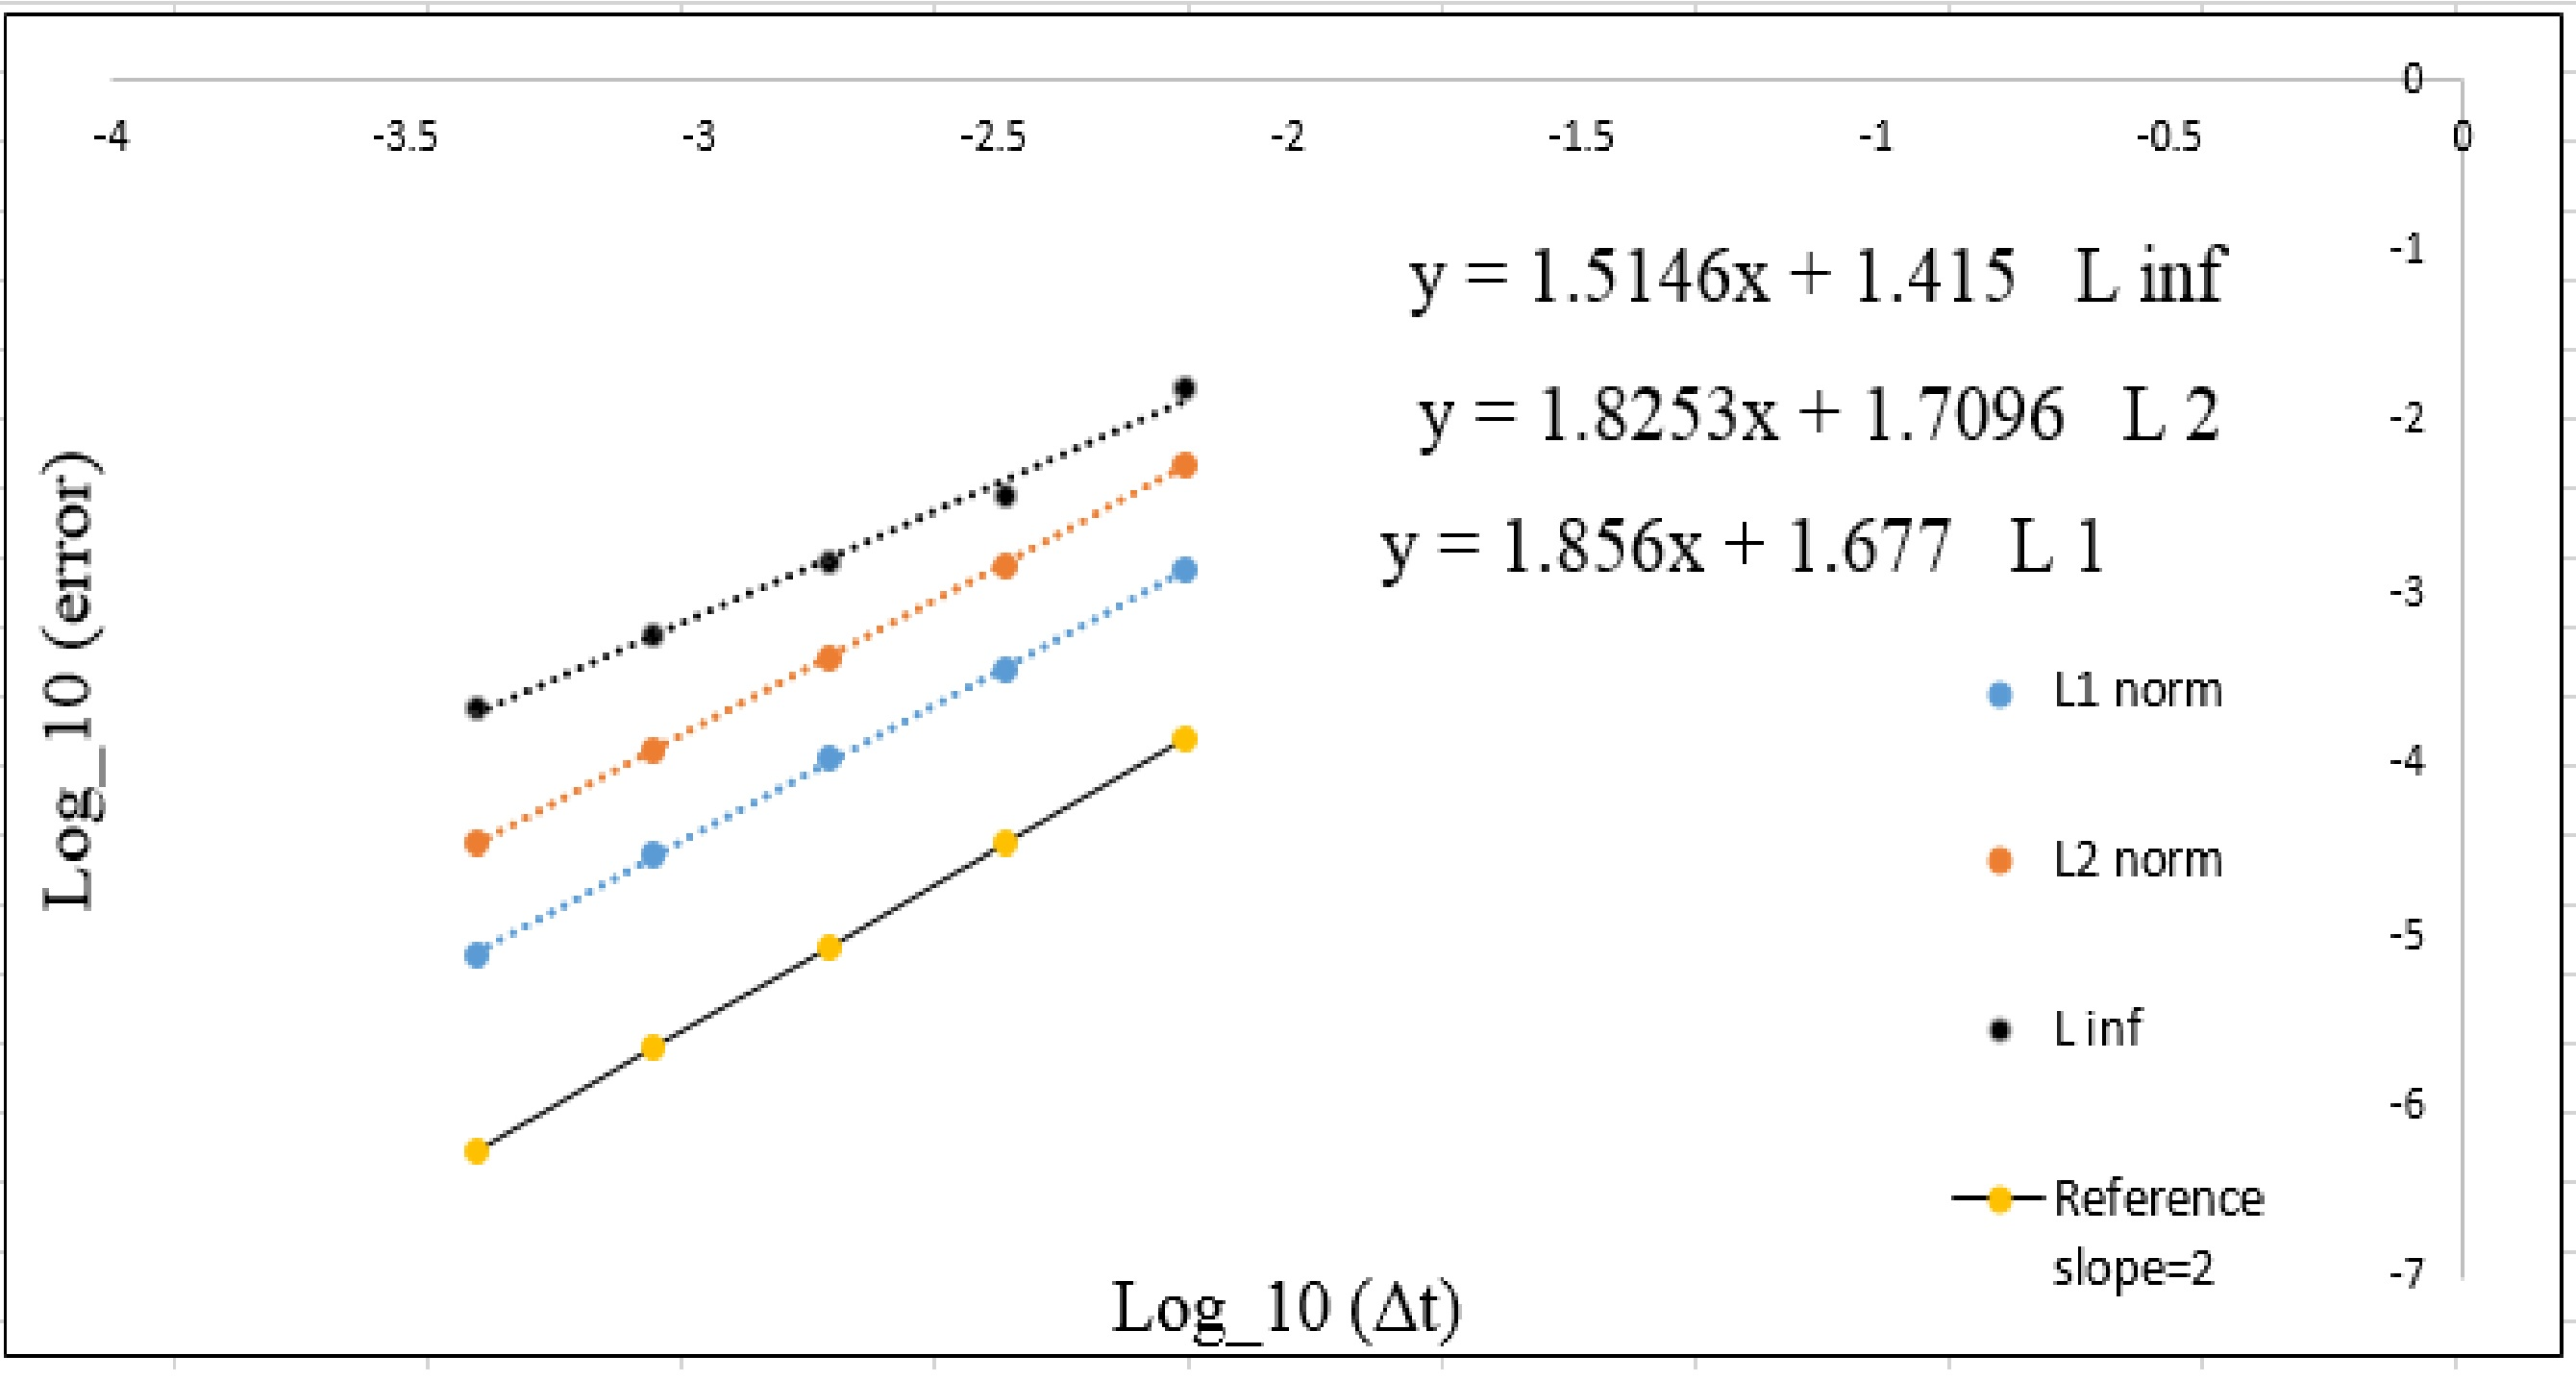
\includegraphics[width=4.5in]{C:/Users/HONGJI/Latex Home directory/Pm1b_pf2b_np_div_uvstar_rate_c_0_5.jpg}
		\caption{Log-Log plot of Convergence rate for $\nabla \cdot \textbf{u}^*$. }\label{fig:6.19b}
	\end{subfigure}
	\caption{Plot of Convergence rates for $Pm\,1\,(b)$ with Normalised Pressure approach used. Domain:  $[-\dfrac{1}{2}, \dfrac{1}{2}]^2$, time = 1 and CFL = 0.5. In each plot, the data points corresponding to grid sizes of 15, 30, 60, 120, 240.}\label{fig:6.16}
\end{figure}

\begin{figure}[H]
	\centering
	\begin{subfigure}[t]{4.5in}
		\centering
		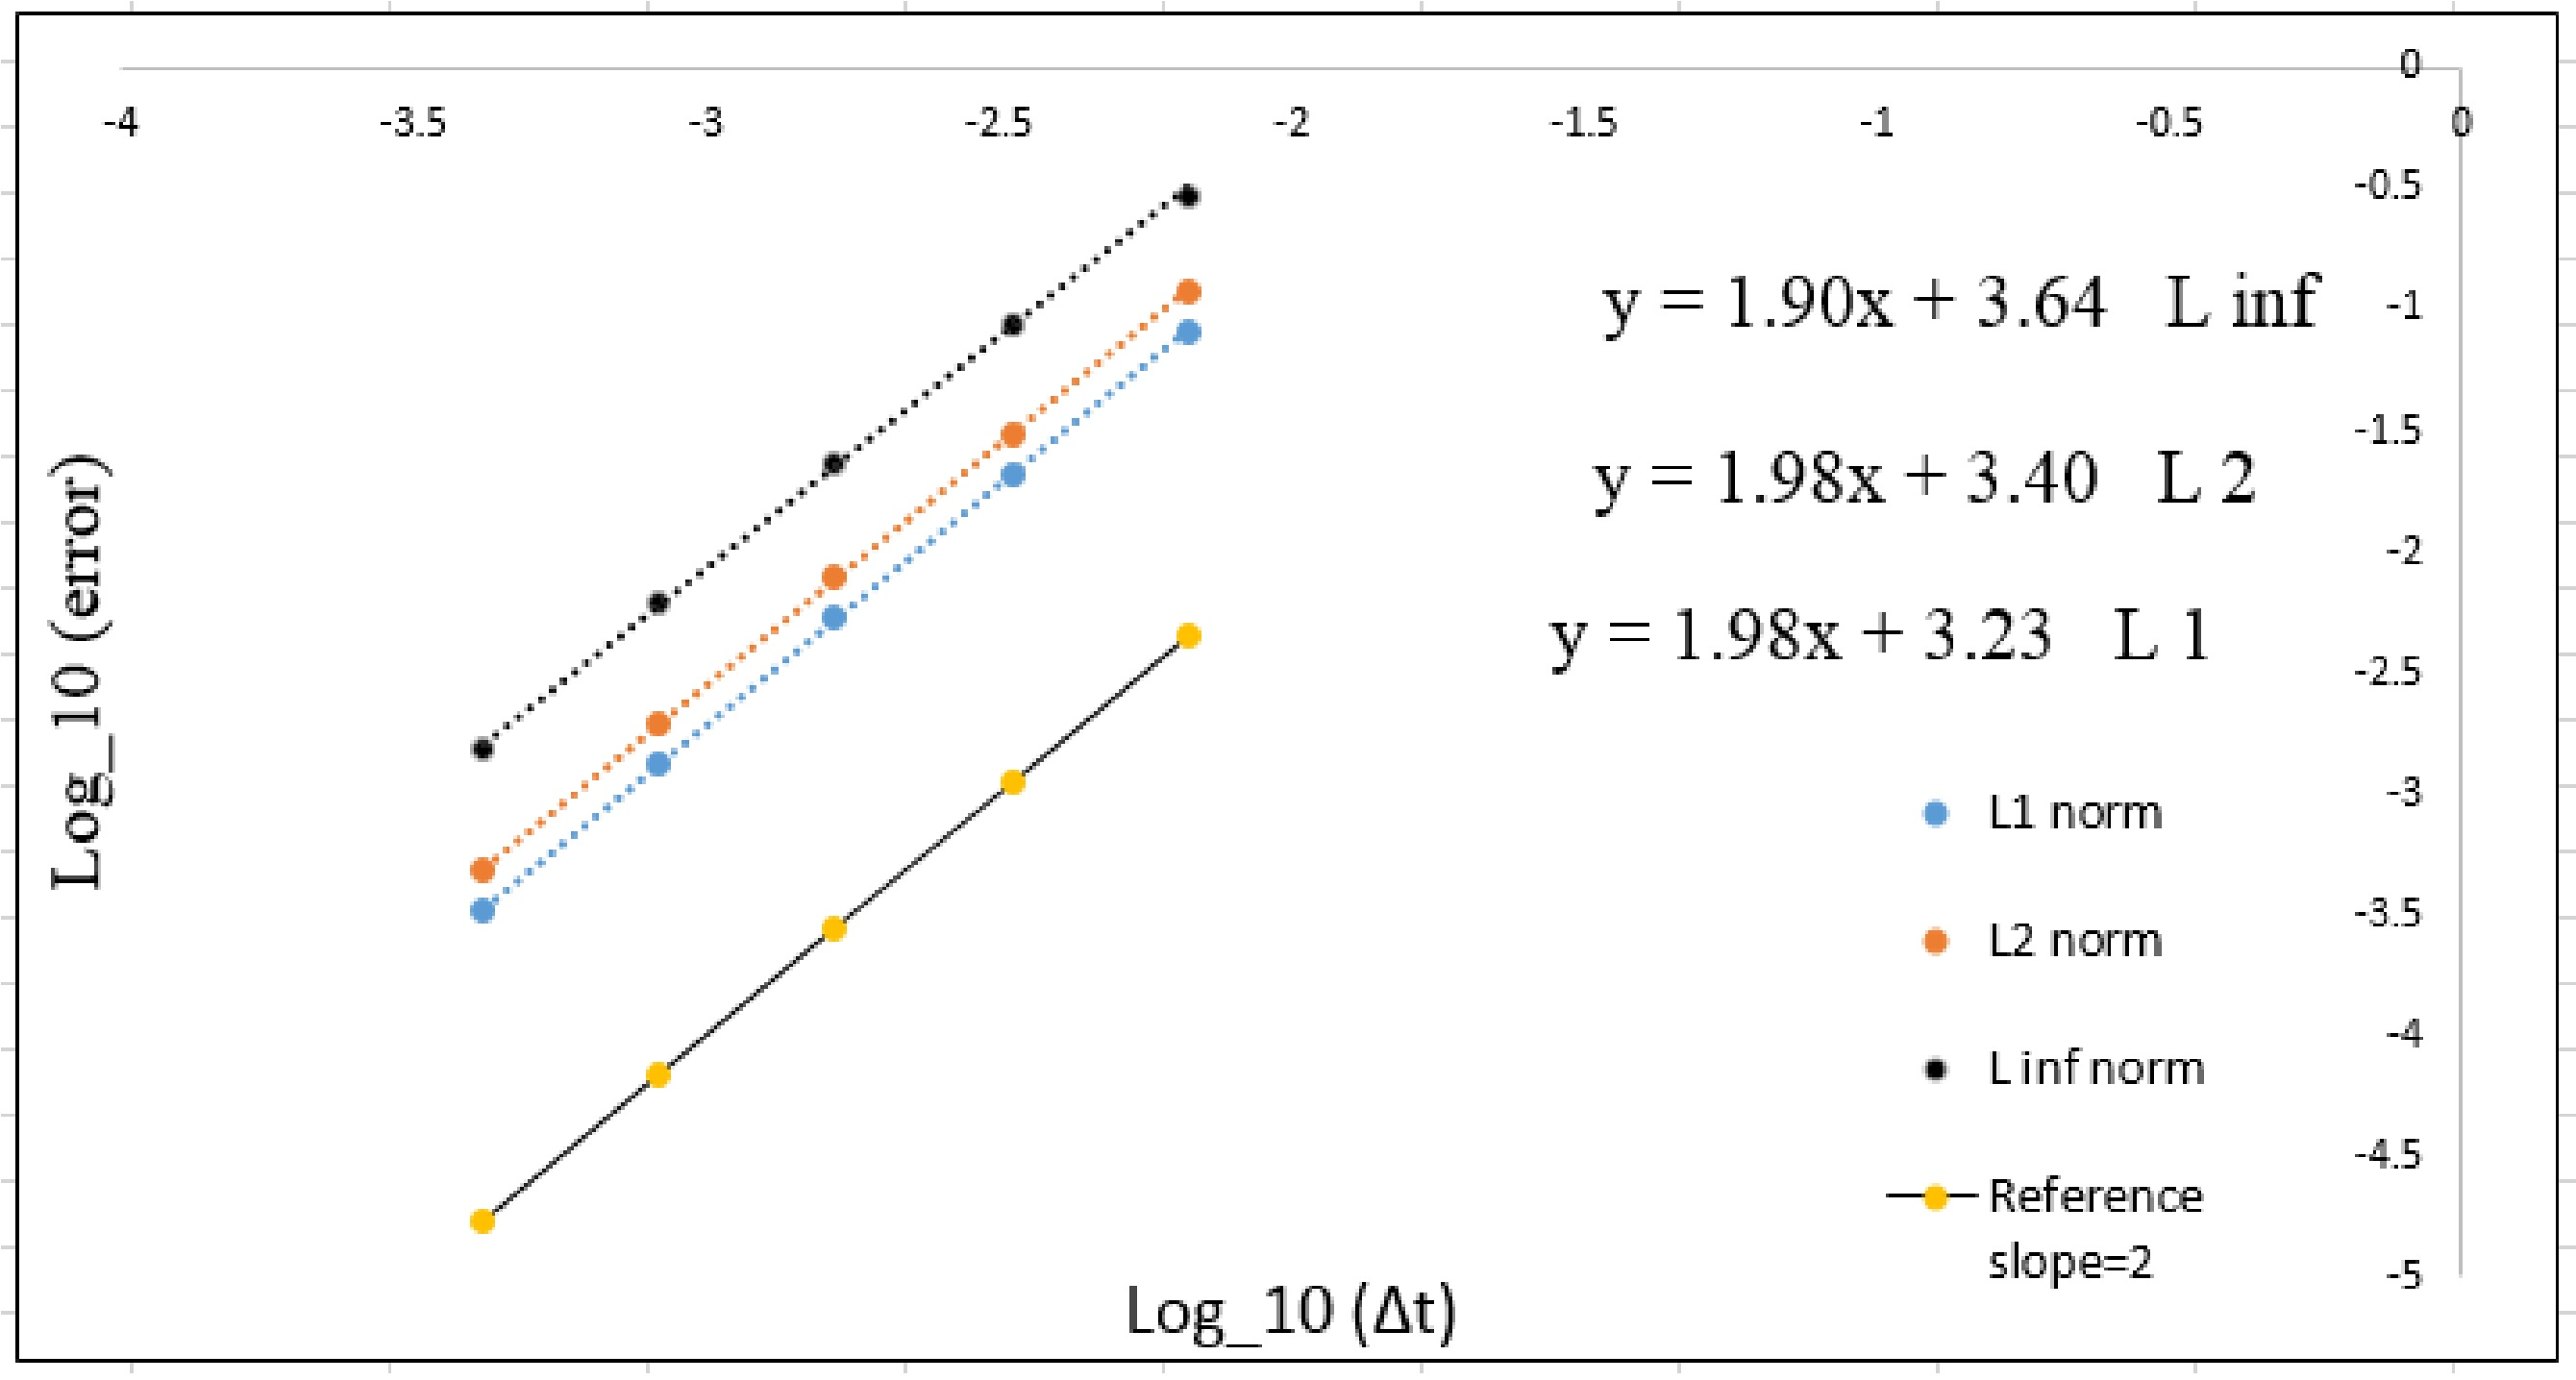
\includegraphics[width=4.5in]{C:/Users/HONGJI/Latex Home directory/Pm2_pf2b_np_P_rate_c_0_5.jpg}
		\caption{Log-Log plot of Convergence rate for Pressure}\label{fig:6.19a}		
	\end{subfigure}
	\quad
	\begin{subfigure}[t]{4.5in}
		\centering
		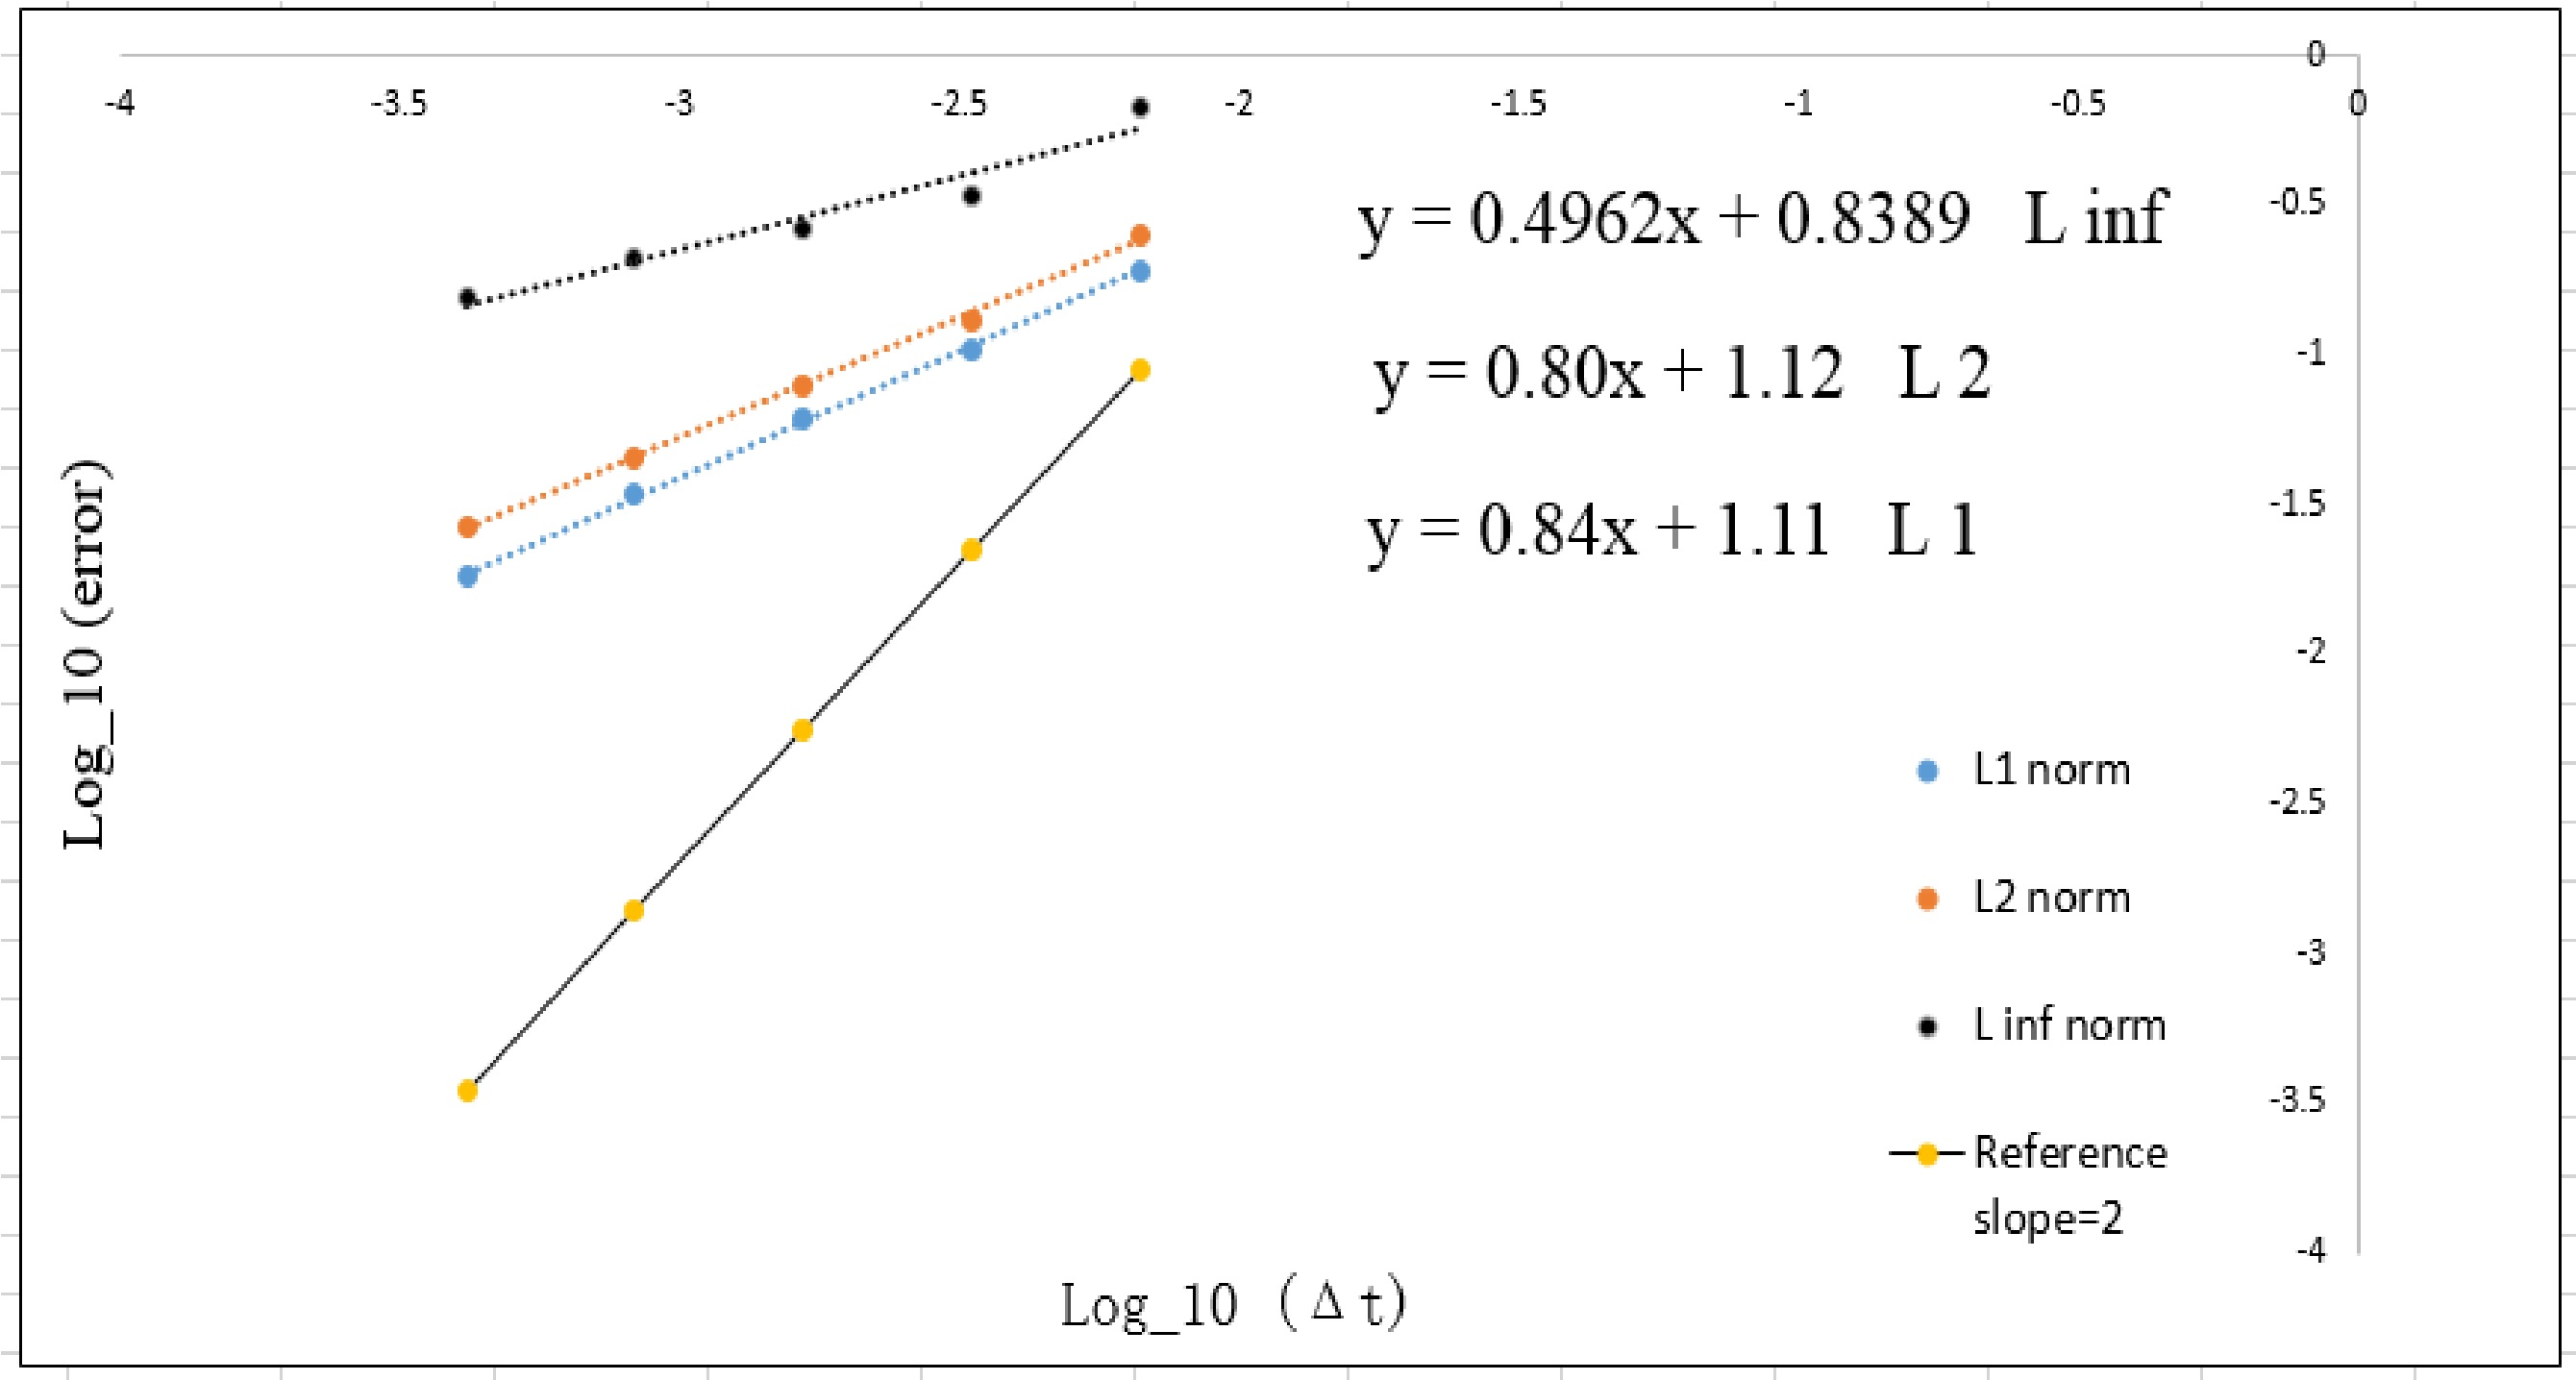
\includegraphics[width=4.5in]{C:/Users/HONGJI/Latex Home directory/Pm2_pf2b_np_div_uvstar_rate_c_0_5.jpg}
		\caption{Log-Log plot of Convergence rate for $\nabla \cdot \textbf{u}^*$. }\label{fig:6.19b}
	\end{subfigure}
	\caption{Plot of Convergence rates for $Pm\,2$ with Normalised Pressure approach used. Domain: $[-\dfrac{1}{2}, \dfrac{1}{2}]^2]^2$, time = 1 and CFL = 0.5. In each plot, the data points corresponding to grid sizes of 15, 30, 60, 120, 240.}\label{fig:6.16}
\end{figure}
\textbf{I will try to add the 480 grid plot too}

\begin{figure}[H]
	\centering
	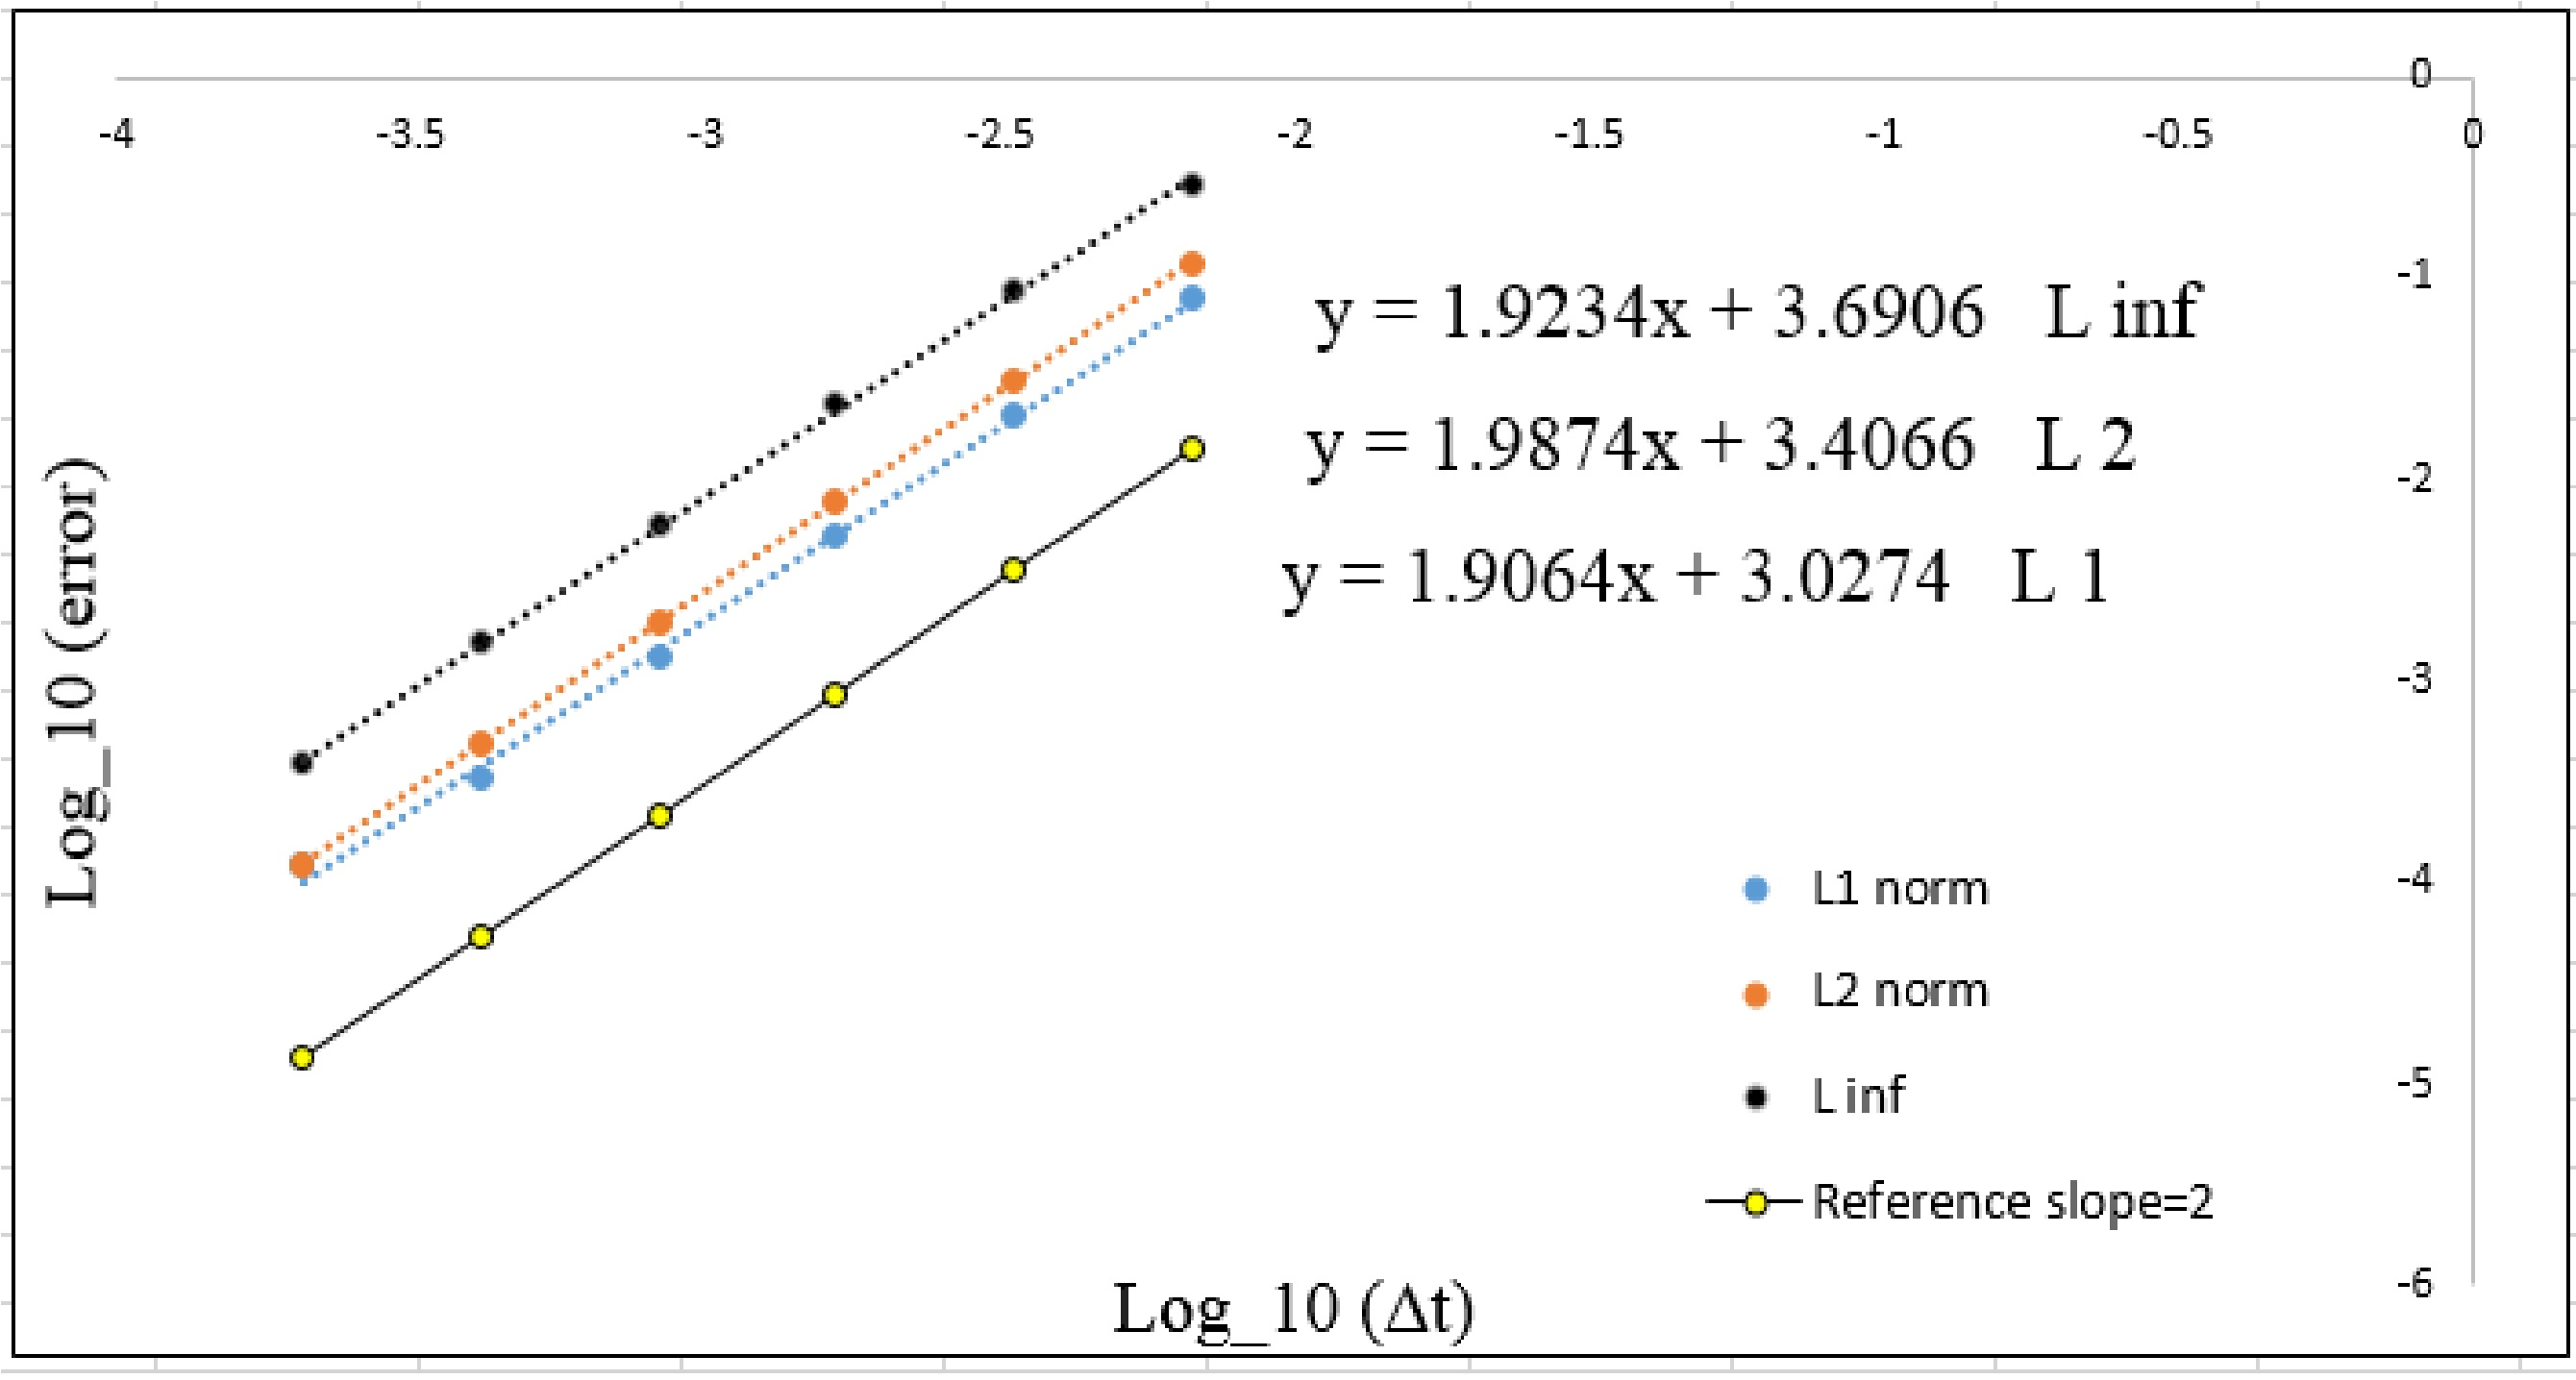
\includegraphics[width=4.5in]{C:/Users/HONGJI/Latex Home directory/Gauge_pf2b_np_P_rate_c_0_5.jpg}
	\caption{Long-Log plot of Pressure Convergence rates for Gauge method with Normalised Pressure approach used. Domain: $[-\dfrac{1}{2},\dfrac{1}{2}]^2$, time = 1 and CFL = 0.5. The data points corresponding to grid sizes of 15, 30, 60, 120, 240, and 480.}\label{fig:6.16}
\end{figure}

\begin{figure}[H]
	\centering
	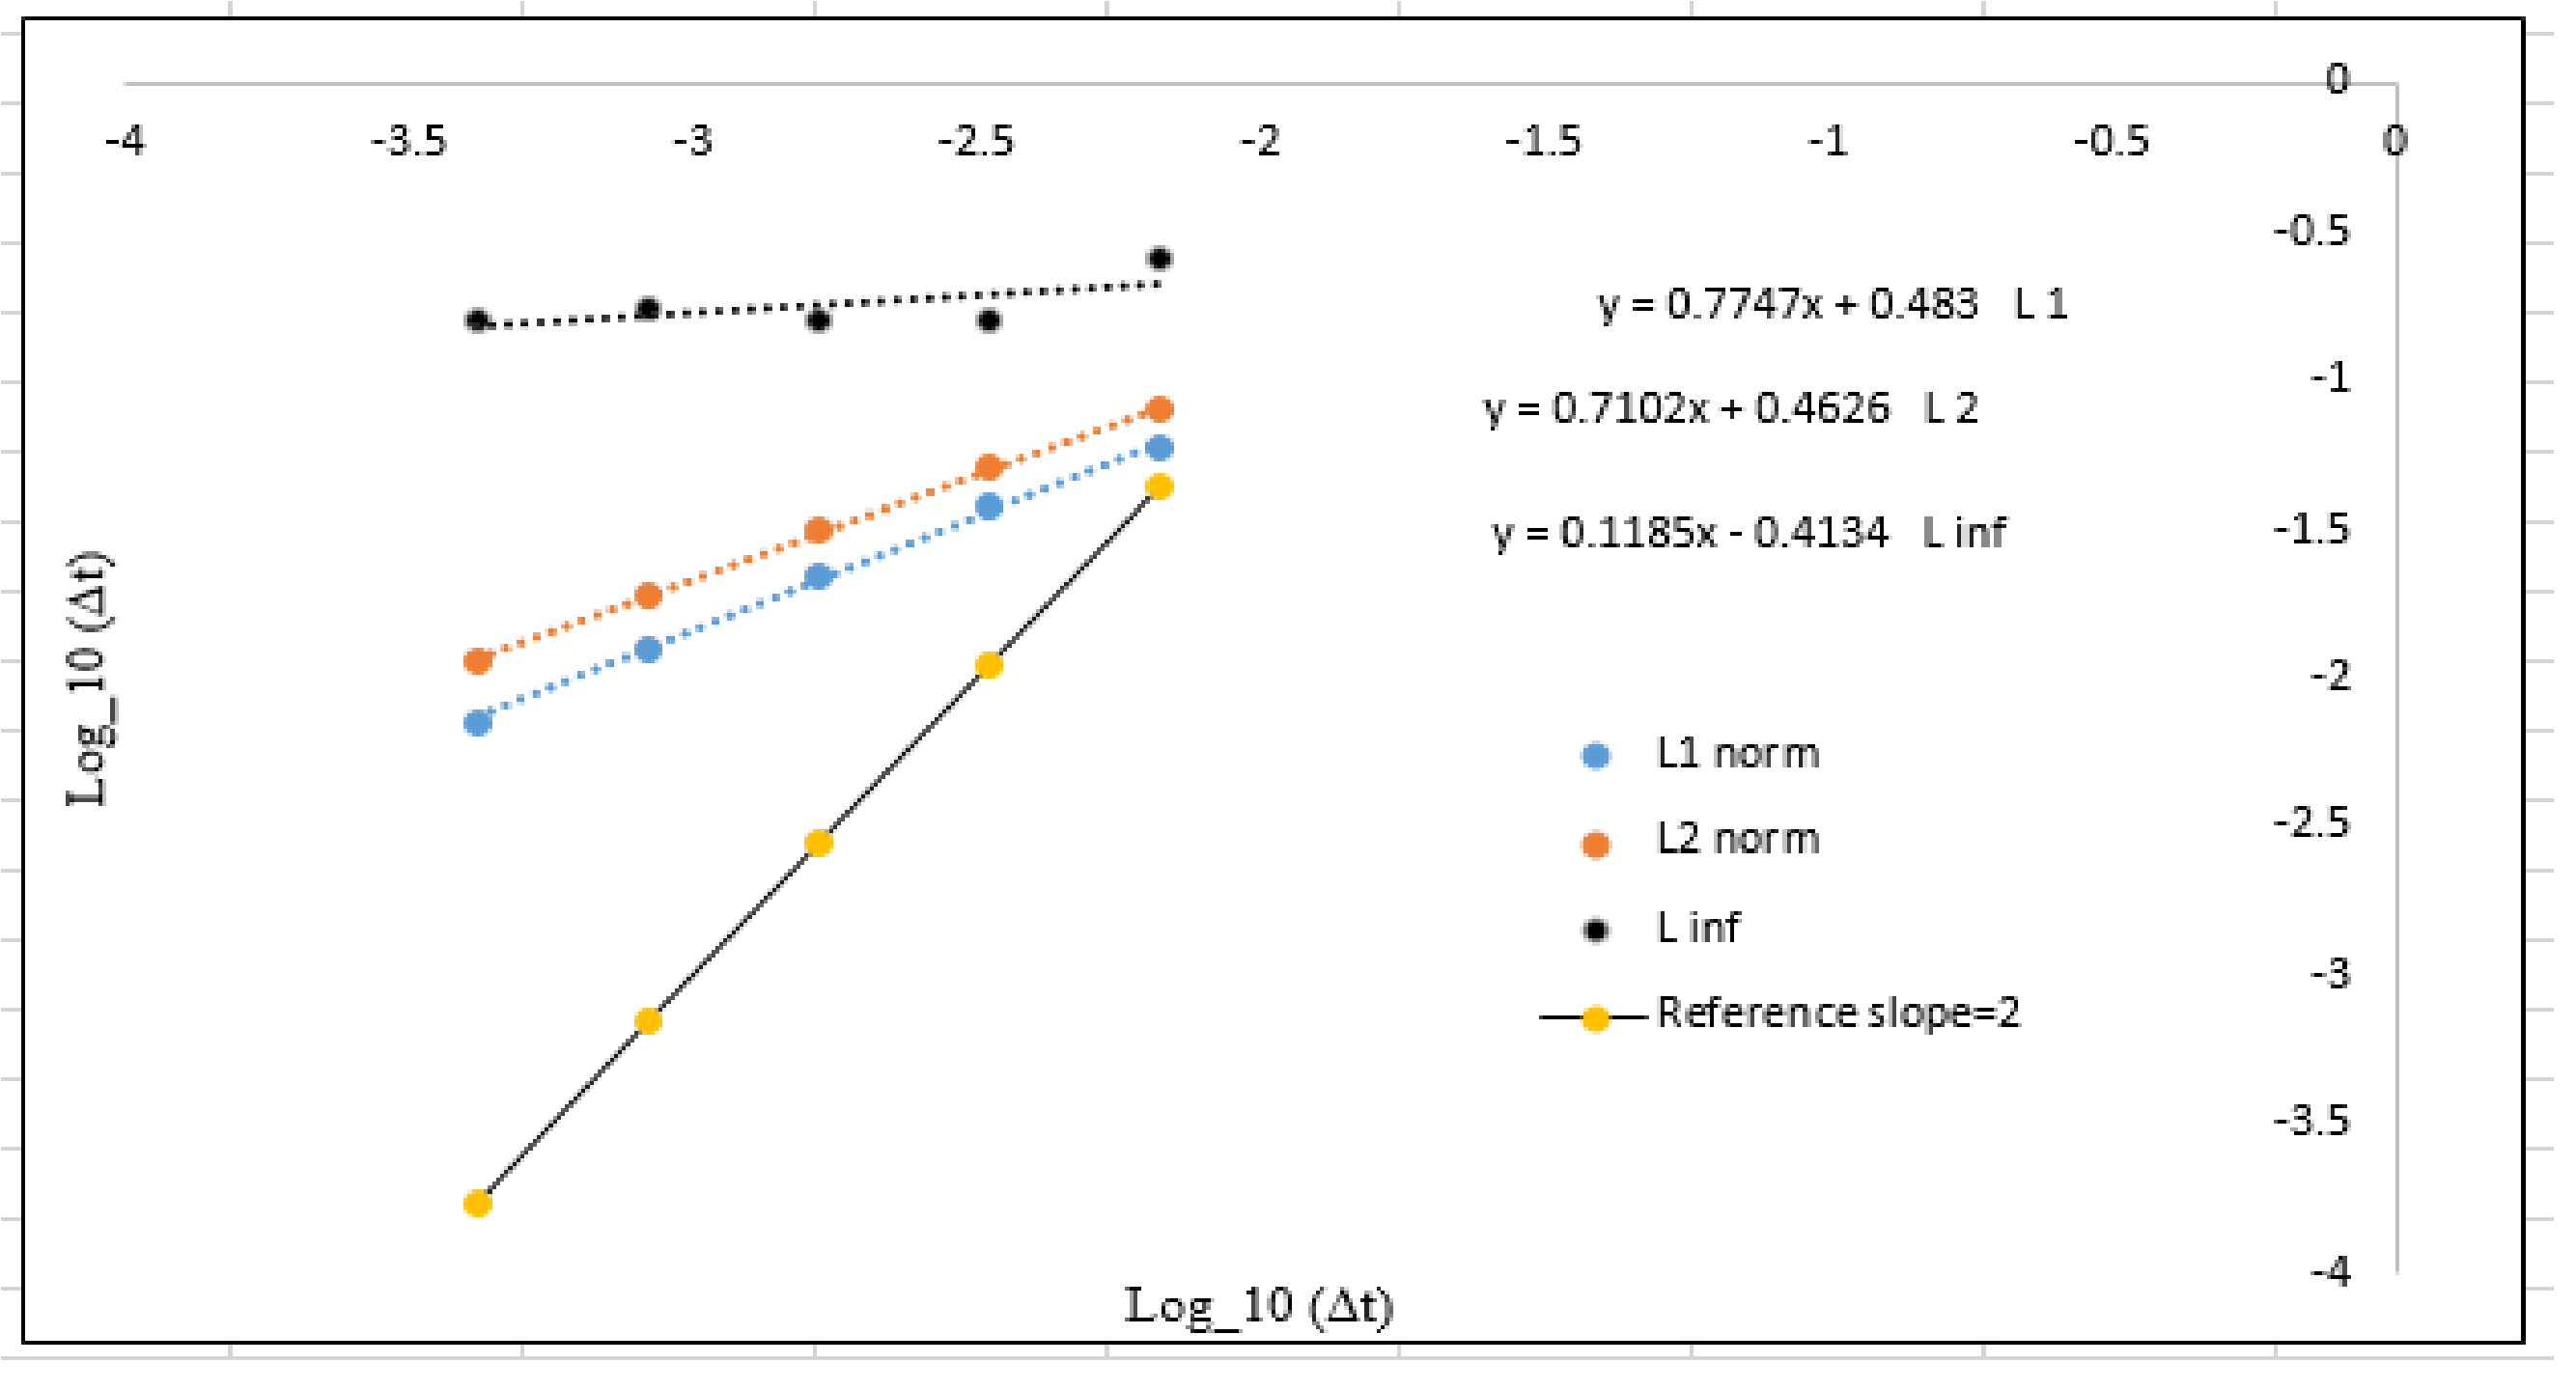
\includegraphics[width=4.5in]{C:/Users/HONGJI/Latex Home directory/Pm2_pf2_cN_np_Dbc_P_error_t_1_grid_120.jpg}
	\caption{Long-Log plot of Pressure Convergence rates for $Pm\,2$ where the less accurate tangential boundary is used. Domain: $[-1,1]^2$, time = 1 and CFL = 0.5. The data points corresponding to grid sizes of 15, 30, 60, 120, 240.}\label{fig:6.16}
\end{figure}

\newpage
To understand why the the non-normalised approach failed to work at fine grids yet provides quite consistent error convergence at small to moderate grids. We have plotted the average of the $\phi$ correction constant for $Pm\,1\,(b)$ method for each grid against the spatial stepping $\Delta x^2$. The plot shows that as we going from coarse grid to finer grid (right to left along the x-axis) the $\phi$ correction generally increases. It reaches a minimum at grid size 60 and the quickly raising up. The reason why it achieves a minimum at grid 60 is still not clear and further investigations are needed. Overall this tells us that the ratio of $\phi$ correction constant and $\Delta x$ becomes larger and larger for finer grids and hence enlarging the error estimate if the constant is not subtracted. This illustrates that the ``Normalised Pressure" approach must be used to guarantee numerical solution convergence. \\

\begin{figure}[H]
	\centering
	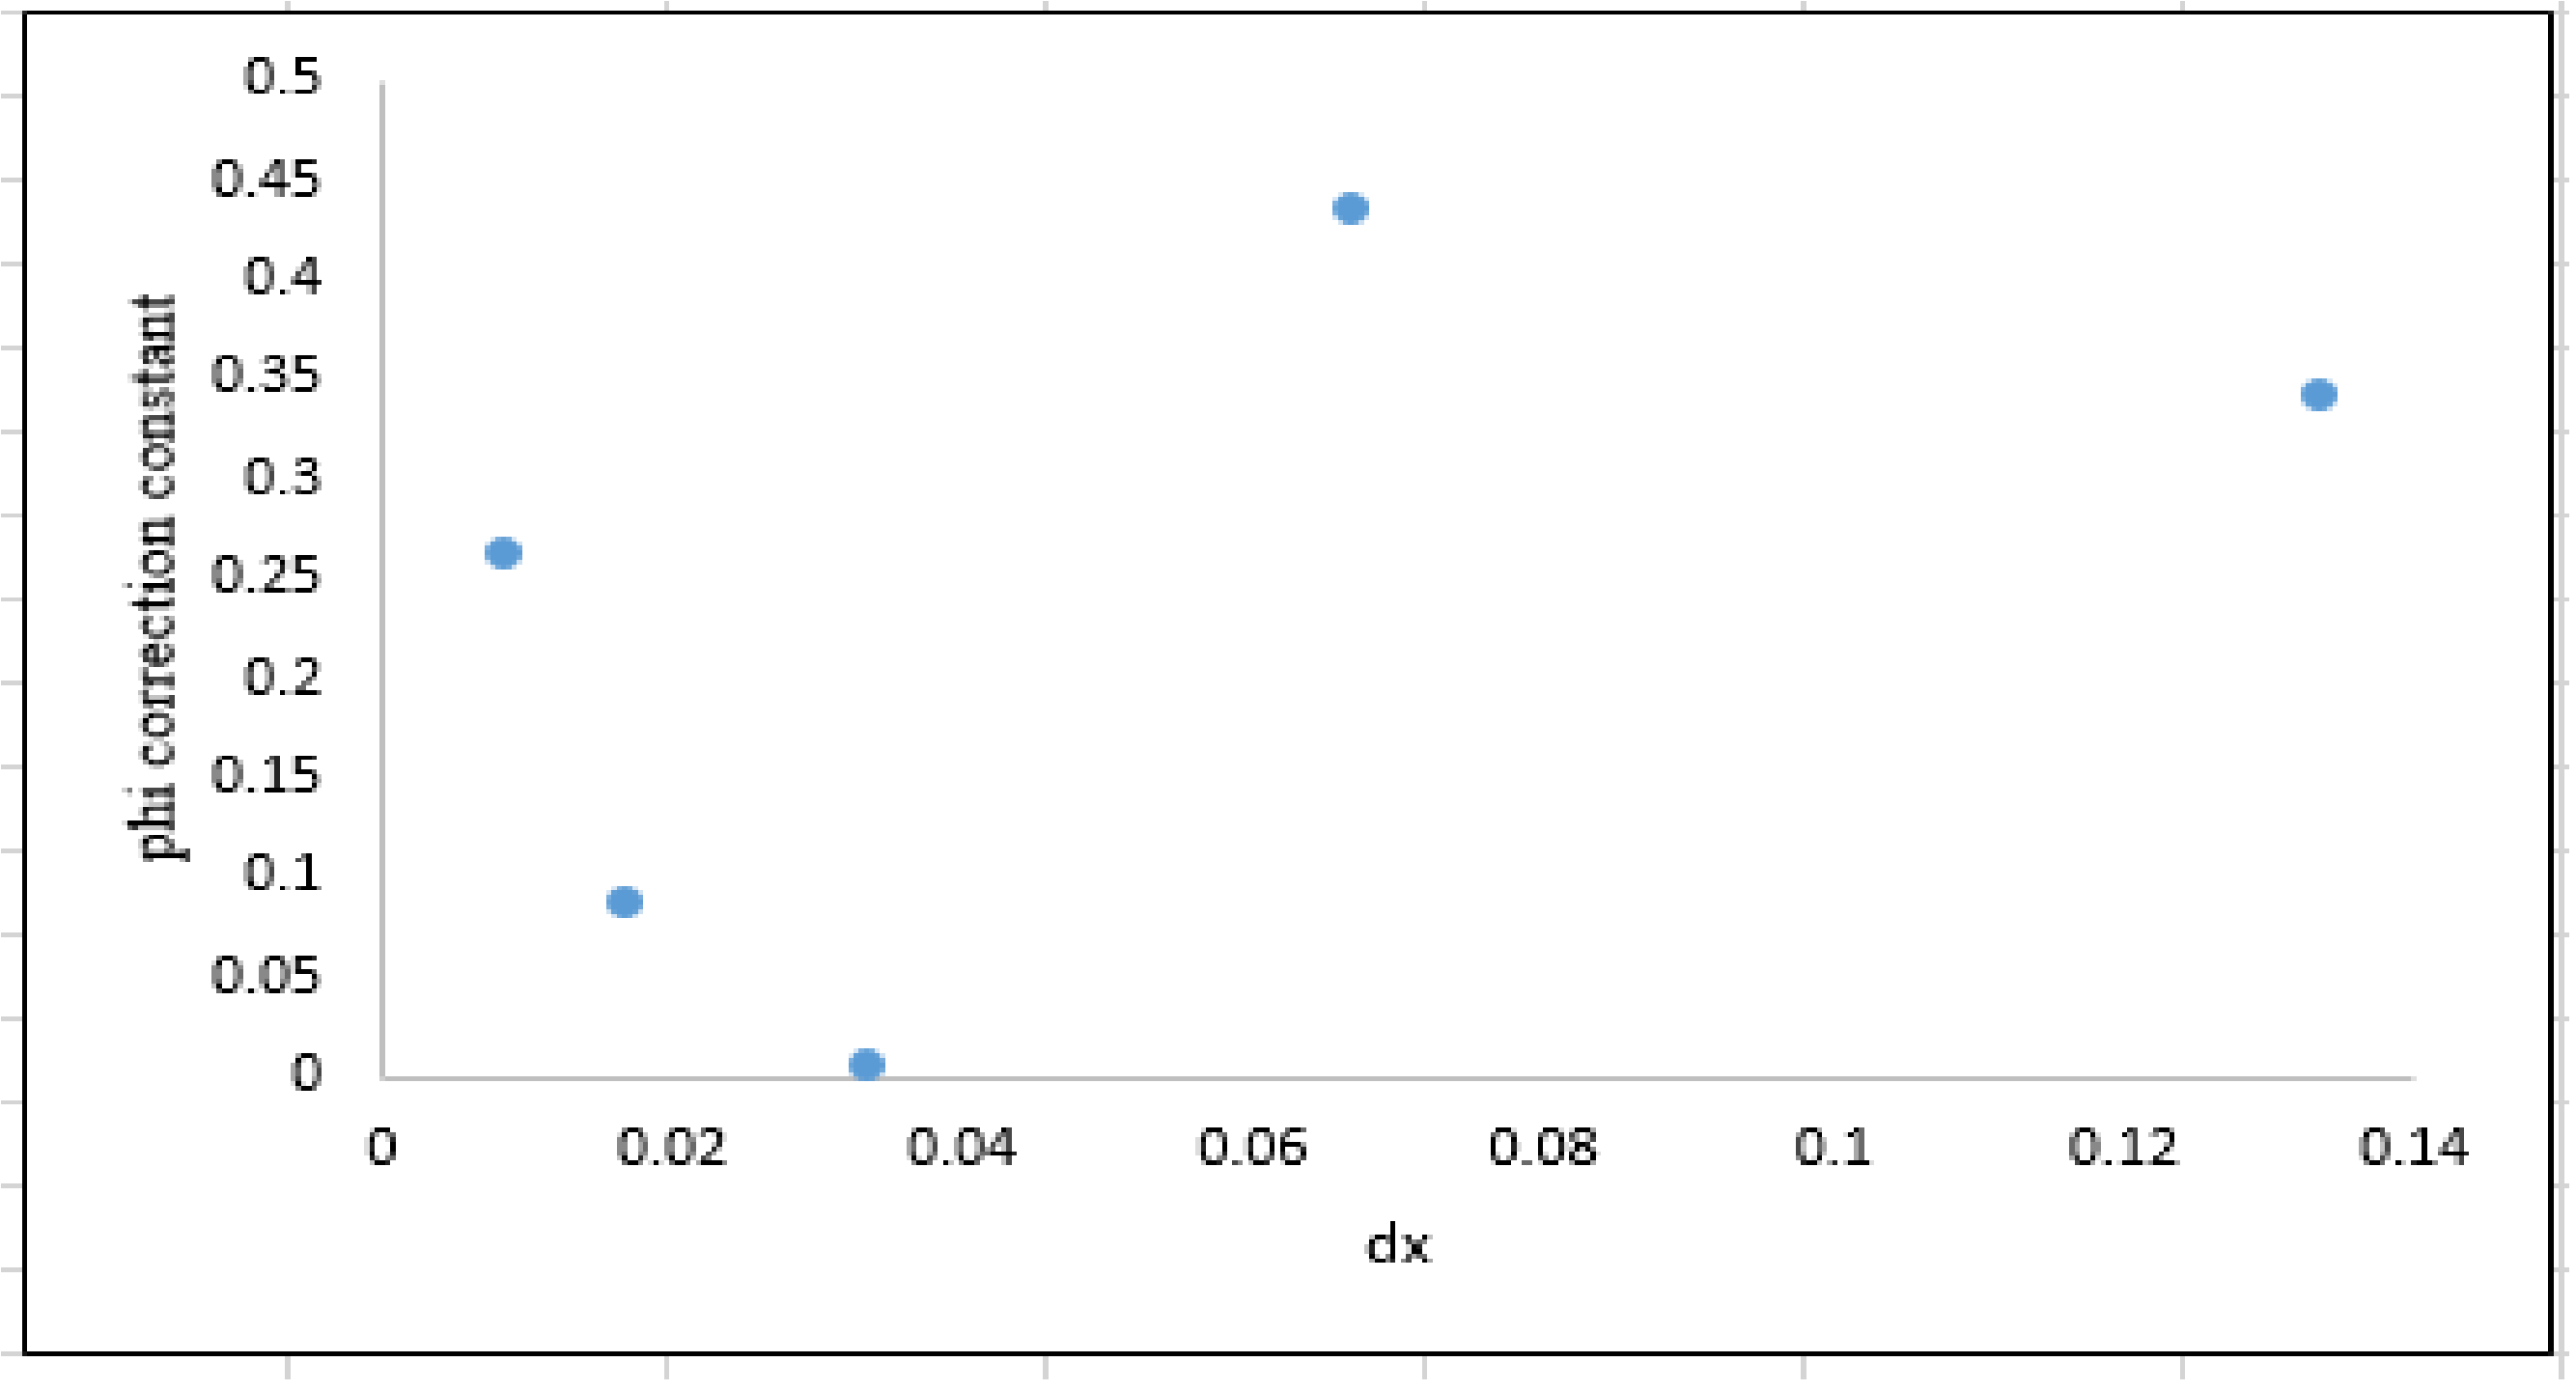
\includegraphics[width=4.5in]{C:/Users/HONGJI/Latex Home directory/Pm1b_pf2_np_phi_c.jpg}
	\caption{Plot of(averaged) $\phi$ correction constant against $\Delta x$ for $Pm\,1\,(b)$ Forced flow on domain: $[-1,1]^2$ and time = 1. CFL = 0.5 was used. The data points corresponding to grid sizes of 15, 30, 60, 120 and 240.}\label{fig:6.16}
\end{figure}

\begin{itemize}
\item Necessity for accurate approximation to $\phi^{n+1}$ along the tangential boundary of the intermediate velocity field.
\end{itemize}

To understand whether $Pm\,2$ behaves better than $Pm\,1\,(b)$ in pressure convergence rates yet it shows a first order convergence in the divergence of intermediate velocity, we need to understand the effect of choice of boundary condition for projection step. In $Pm\,1\,(b)$ no approximation to $\phi^{n+1}$ were used when computing $\textbf{u}^*$ along the tangential boundary whereas in $Pm\,2$ second order approximation to $\phi^{n+1}$ were used. The tangential boundary for $\textbf{u}^*$ is therefore $\textbf{$\tau$} \cdot \nabla (2\phi^n - \phi^{n-1})$ ($(2\phi^n - \phi^{n-1})$ approximates $\phi^{n+1}$). We now rerun $Pm\,2$ with the less accurate boundary where $\textbf{$\tau$} \cdot \textbf{u}^* = \textbf{$\tau$} \cdot \textbf{u}^{n+1}$ (as in $Pm\,1\,(b)$). The convergence rates in pressure are again summarised in Figure below. It is observed that the rates are much reduced to about 0.7 order. This is because the numerical boundary in $\textbf{u}^*$ is very big. This finding indicates that for $Pm\,2$ accurate approximation to $\phi^{n+1}$ must be implemented when computing the intermediate velocity field along the boundary points. This is consistent with the findings of \emph{David et.al} \cite{brown2001accurate}.

\subsection{Unforced flow problem}

To test the effect of smoothness of domain to the accuracy of projection methods. Another unforced flow problem is also considered. It is the well-known 2-D Taylor solution to the Navier Stokes equations. The analytic solutions are:

\begin{dgroup}
\begin{dmath}
u = -\cos(x)\sin(y)e^{-2t}
\end{dmath}
\begin{dmath}
v = \sin(x)\cos(y)e^{-2t}
\end{dmath}
\begin{dmath}
p = -\dfrac{1}{4\,Re}(\cos(2x)+\cos(2y))e^{-4t}
\end{dmath}
\end{dgroup}

This test problem has non-trivial boundary conditions for velocities and non-trivial pressure gradients, unlike the forced flow exampled we have considered before where 2 of its boundaries are zero for velocities and pressure. Hence this should reveal more information on how the projection methods depends on the structure of domain and boundary conditions. For simplicity let's consider the domain: $[-\dfrac{\pi}{4}, \dfrac{\pi}{4}]^2$. Then the pressure value at these 4 corners ($x = \pm \dfrac{\pi}{4}$ and $y = \pm \dfrac{\pi}{4}$) would then be zero for all times which makes our pressure normalisation process easier.\\

We use these corner points to calculate the best possible $\phi$ correction constant and subtract it from the numerical $\phi$ obtained by solving the Poisson equation. This recovers the exact $\phi$ we want. Much the same process as we did in the forced flow example.\\

In addition, this Taylor solutions are derived from the full Navier Stokes equations and hence it is also good to test our convective term solvers too.\\

We have again run the Projection methods and Gauge for 5 grid sizes from $15 \times 15$ to $240 \times 240$. The spatial stepping is half each time. The solutions are calculated at time 0.1s and with Reynolds number equals to 1. A CFL number of 0.05 is used in all methods to obtain better error estimates.\\

The convergence rates in pressure are summarised in Figure. Interestingly all the methods show fully second order convergence except for $Pm\,1\,(b)$ where only first order convergence is observed. This time all the norms show degraded accuracy. Take a look at the Pressure error field we observe very large spikes located at the 4 corners of the domain. This indicates the Presence of numerical boundary layers which are manifested better in the plot of Divergence of intermediate velocity field. Interestingly the magnitude of divergence of numerical boundary in intermediate velocity field is even larger for $Pm\,2$ yet resulting in small Pressure error field. This result shows that the numerical boundary layers in $\phi$ and $\nabla \cdot \textbf{u}^*$ cannot be fully filtered out in the projection methods unless accurate boundary condition for $\textbf{$\tau$} \cdot \textbf{u}^*$ is implemented. The boundary layers are only partially filtered out by the pressure update formula (equation 6.) which was proposed by \emph{David et.al} \cite{brown2001accurate}. This is illustrated by the surface plots in $Pm\,1\,(b)$ where the thick boundary layer in $\nabla \cdot \textbf{u}^*$ is eliminated in Pressure but the 4 spikes still present. The pressure error  in $Pm\,2$  however is much more smooth. This clearly illustrates the importance or ``necessity" for accurate boundary condition for the tangential component of intermediate velocity in order to achieve fully second order convergence in pressure. This finding is also consistent with that obtained in \emph{David et.al} \cite{brown2001accurate}.\\

The exact reason of why $Pm\,1\,(b)$ shows such a significant reduction in accuracy whereas other methods like $Pm\,2$ give optimal results still remains puzzling. Take a look at the pressure update formula between the two methods we find that the only difference is the pressure approximation $q$ where $Pm\,1\,(b)$ used the pressure at previous time step and $Pm\,2$ and uses no approximation at all. Hence we infer that it is choice of pressure approximation $q$ which limits the accuracy in $Pm\,1\,(b)$. Recall in normal mode analysis, we showed that through the definition of $\phi$ by the relation: $q = Q(n)\phi$ we can eliminate the numerical boundary layer with the new update formula. However this relation gives a very worrying normal pressure gradient.\\

Since $q = Q(n)\phi$ and the normal gradient of $\phi$ is zero resulting from projection. Hence the pressure approximation $q$ and consequently the pressure at previous step has a zero Neumann boundary condition. 
\begin{equation}
\textbf{n} \cdot \nabla q = \textbf{n} \cdot \nabla p^{n-1/2} = Q(n) \textbf{n}\cdot \nabla \phi = 0
\end{equation}

This is not only inconsistent with what was implied by the pressure update formula but also inconsistent with the true normal pressure gradient. In our unforced problem, the normal pressure gradient at west boundary ($x=\dfrac{\pi}{4}$ at any time is: $\dfrac{1}{2}\left(-\sin(\dfrac{\pi}{4}\right)$ which is obviously not zero. Hence this means this choice of $q$ does not work properly at the boundary.\\

It is supported by the plot of normal pressure gradient at West boundary. The plot of numerical solution is  different to that of the analytical solution. This is amplified at the 4 corners of the domain where large spikes occur. We therefore infer that it is the non-smoothness caused by the inconsistent pressure approximation which degrades the global convergence of $Pm\,1\,(b)$.\\

We propose a simplified way and modification to solve $q$ 
\begin{equation}
q = 2\phi^{n-1/2} - \phi^{n-3/2}.
\end{equation}

This results in a more consistent normal pressure gradient: $2\phi^{n-1/2} - \phi{n-3/2}$. Moreover it represents a second order approximation to $p^{n+1/2}$. This can be shown using a simple Taylor series argument. With this modified pressure approximation $q$, the numerical normal pressure gradient now approximates the analytic one better. It is converging to the analytic pressure gradient at a second order rate. The non-smooth spikes are now eliminated which reduces the error and also lifts up the global pressure error convergence to 2.5 order.\\

\begin{figure}[H]
	\centering
	\begin{subfigure}[t]{4.5in}
		\centering
		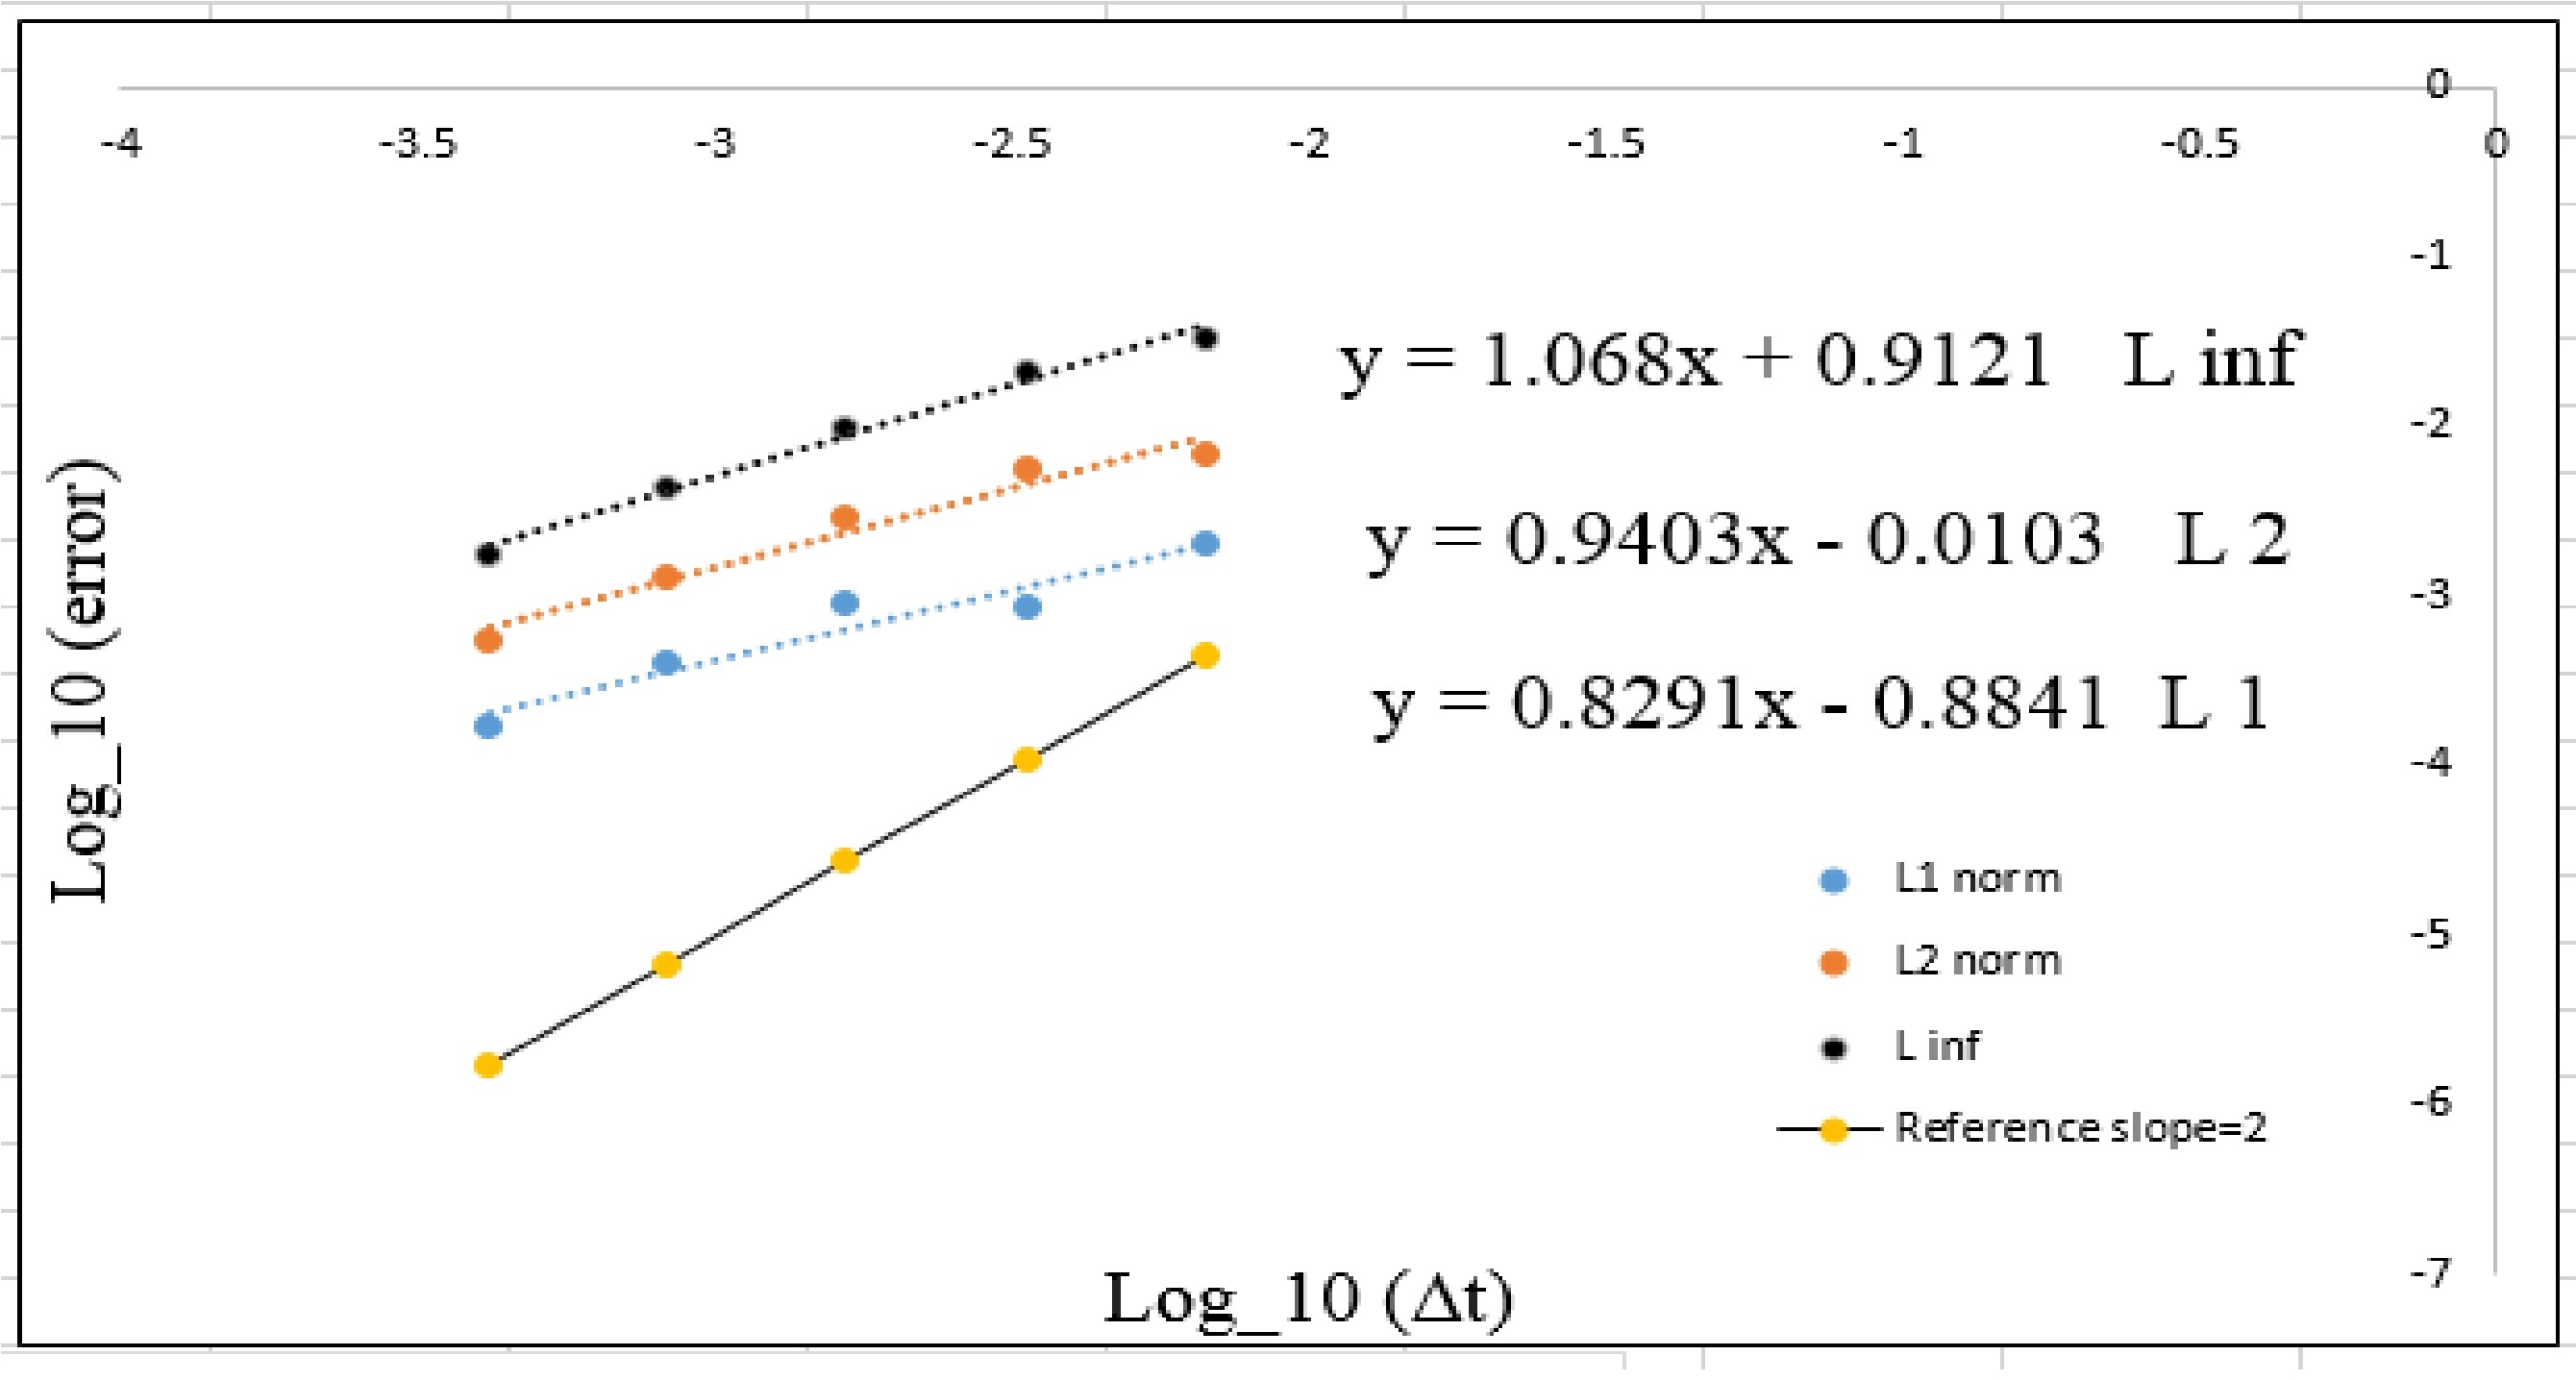
\includegraphics[width=4.5in]{C:/Users/HONGJI/Latex Home directory/Pm1b_unf1_np_P_rate.jpg}
		\caption{Log-Log plot of Convergence rate for Pressure $Pm\,1\,(b)$ method}\label{fig:6.19a}		
	\end{subfigure}
	\quad
	\begin{subfigure}[t]{4.5in}
		\centering
		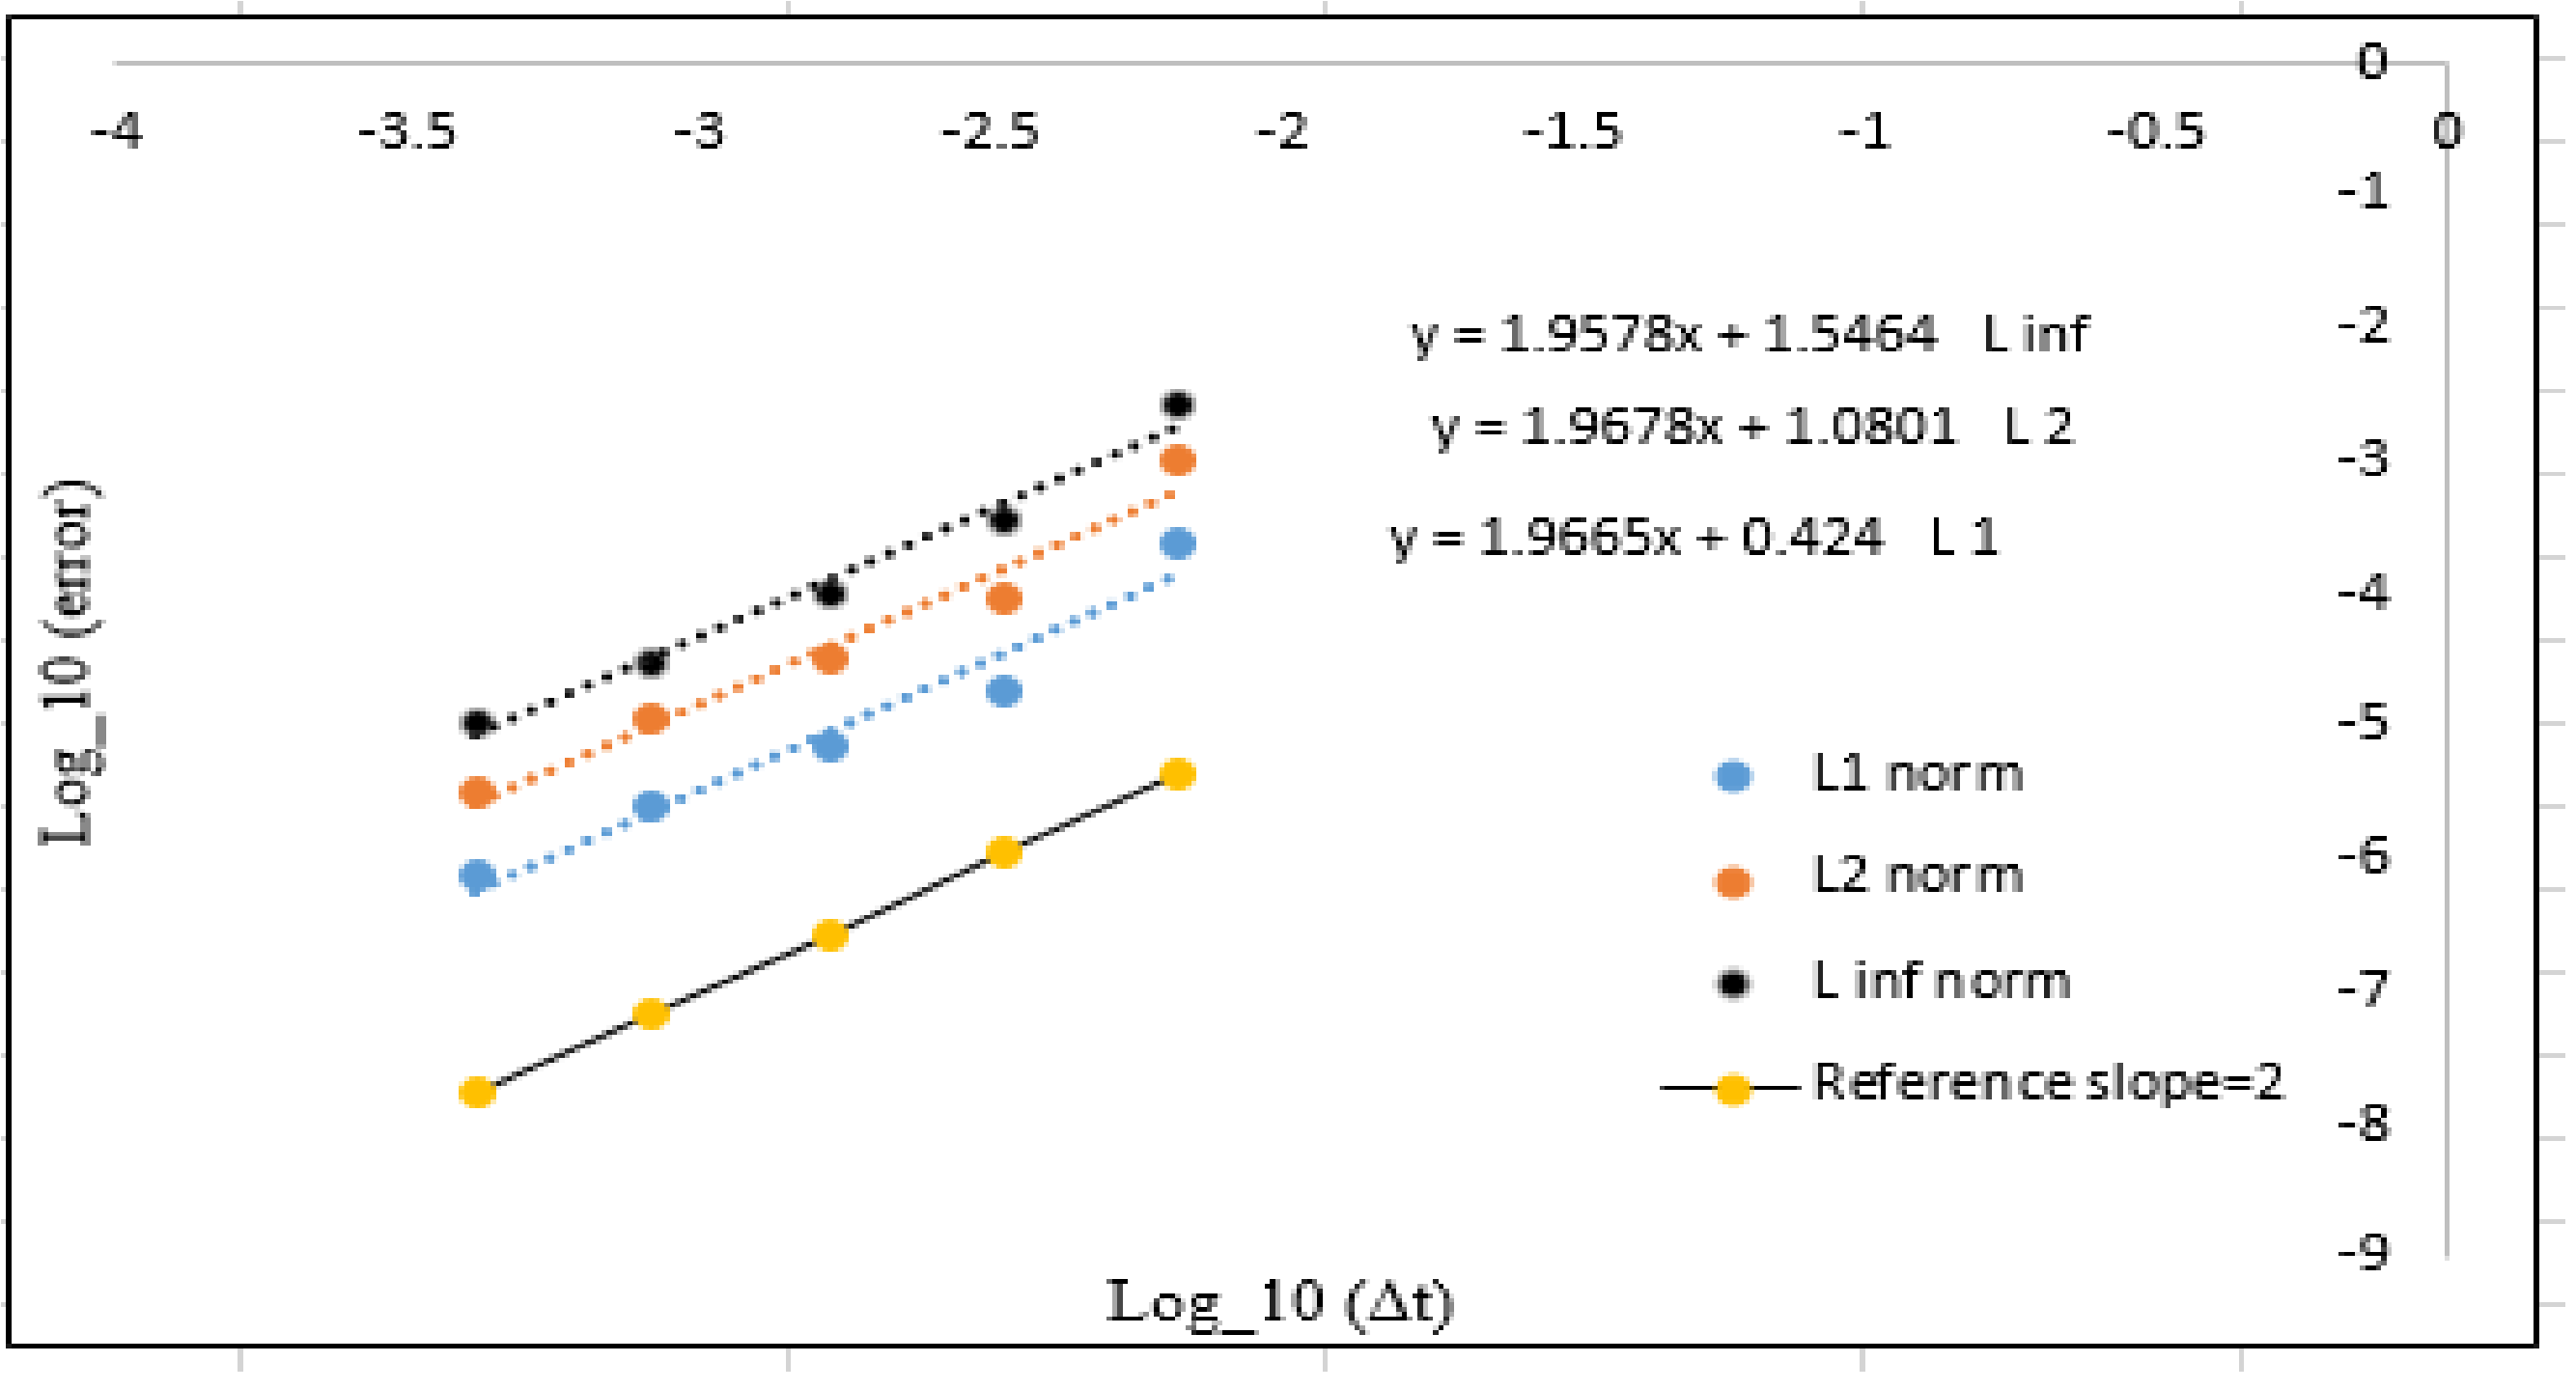
\includegraphics[width=4.5in]{C:/Users/HONGJI/Latex Home directory/Pm2_unf1_np_P_rate.jpg}
		\caption{Log-Log plot of Convergence rate for Pressure $Pm\,2$. }\label{fig:6.19b}
	\end{subfigure}
	\quad
	\begin{subfigure}[t]{4.5in}
		\centering
		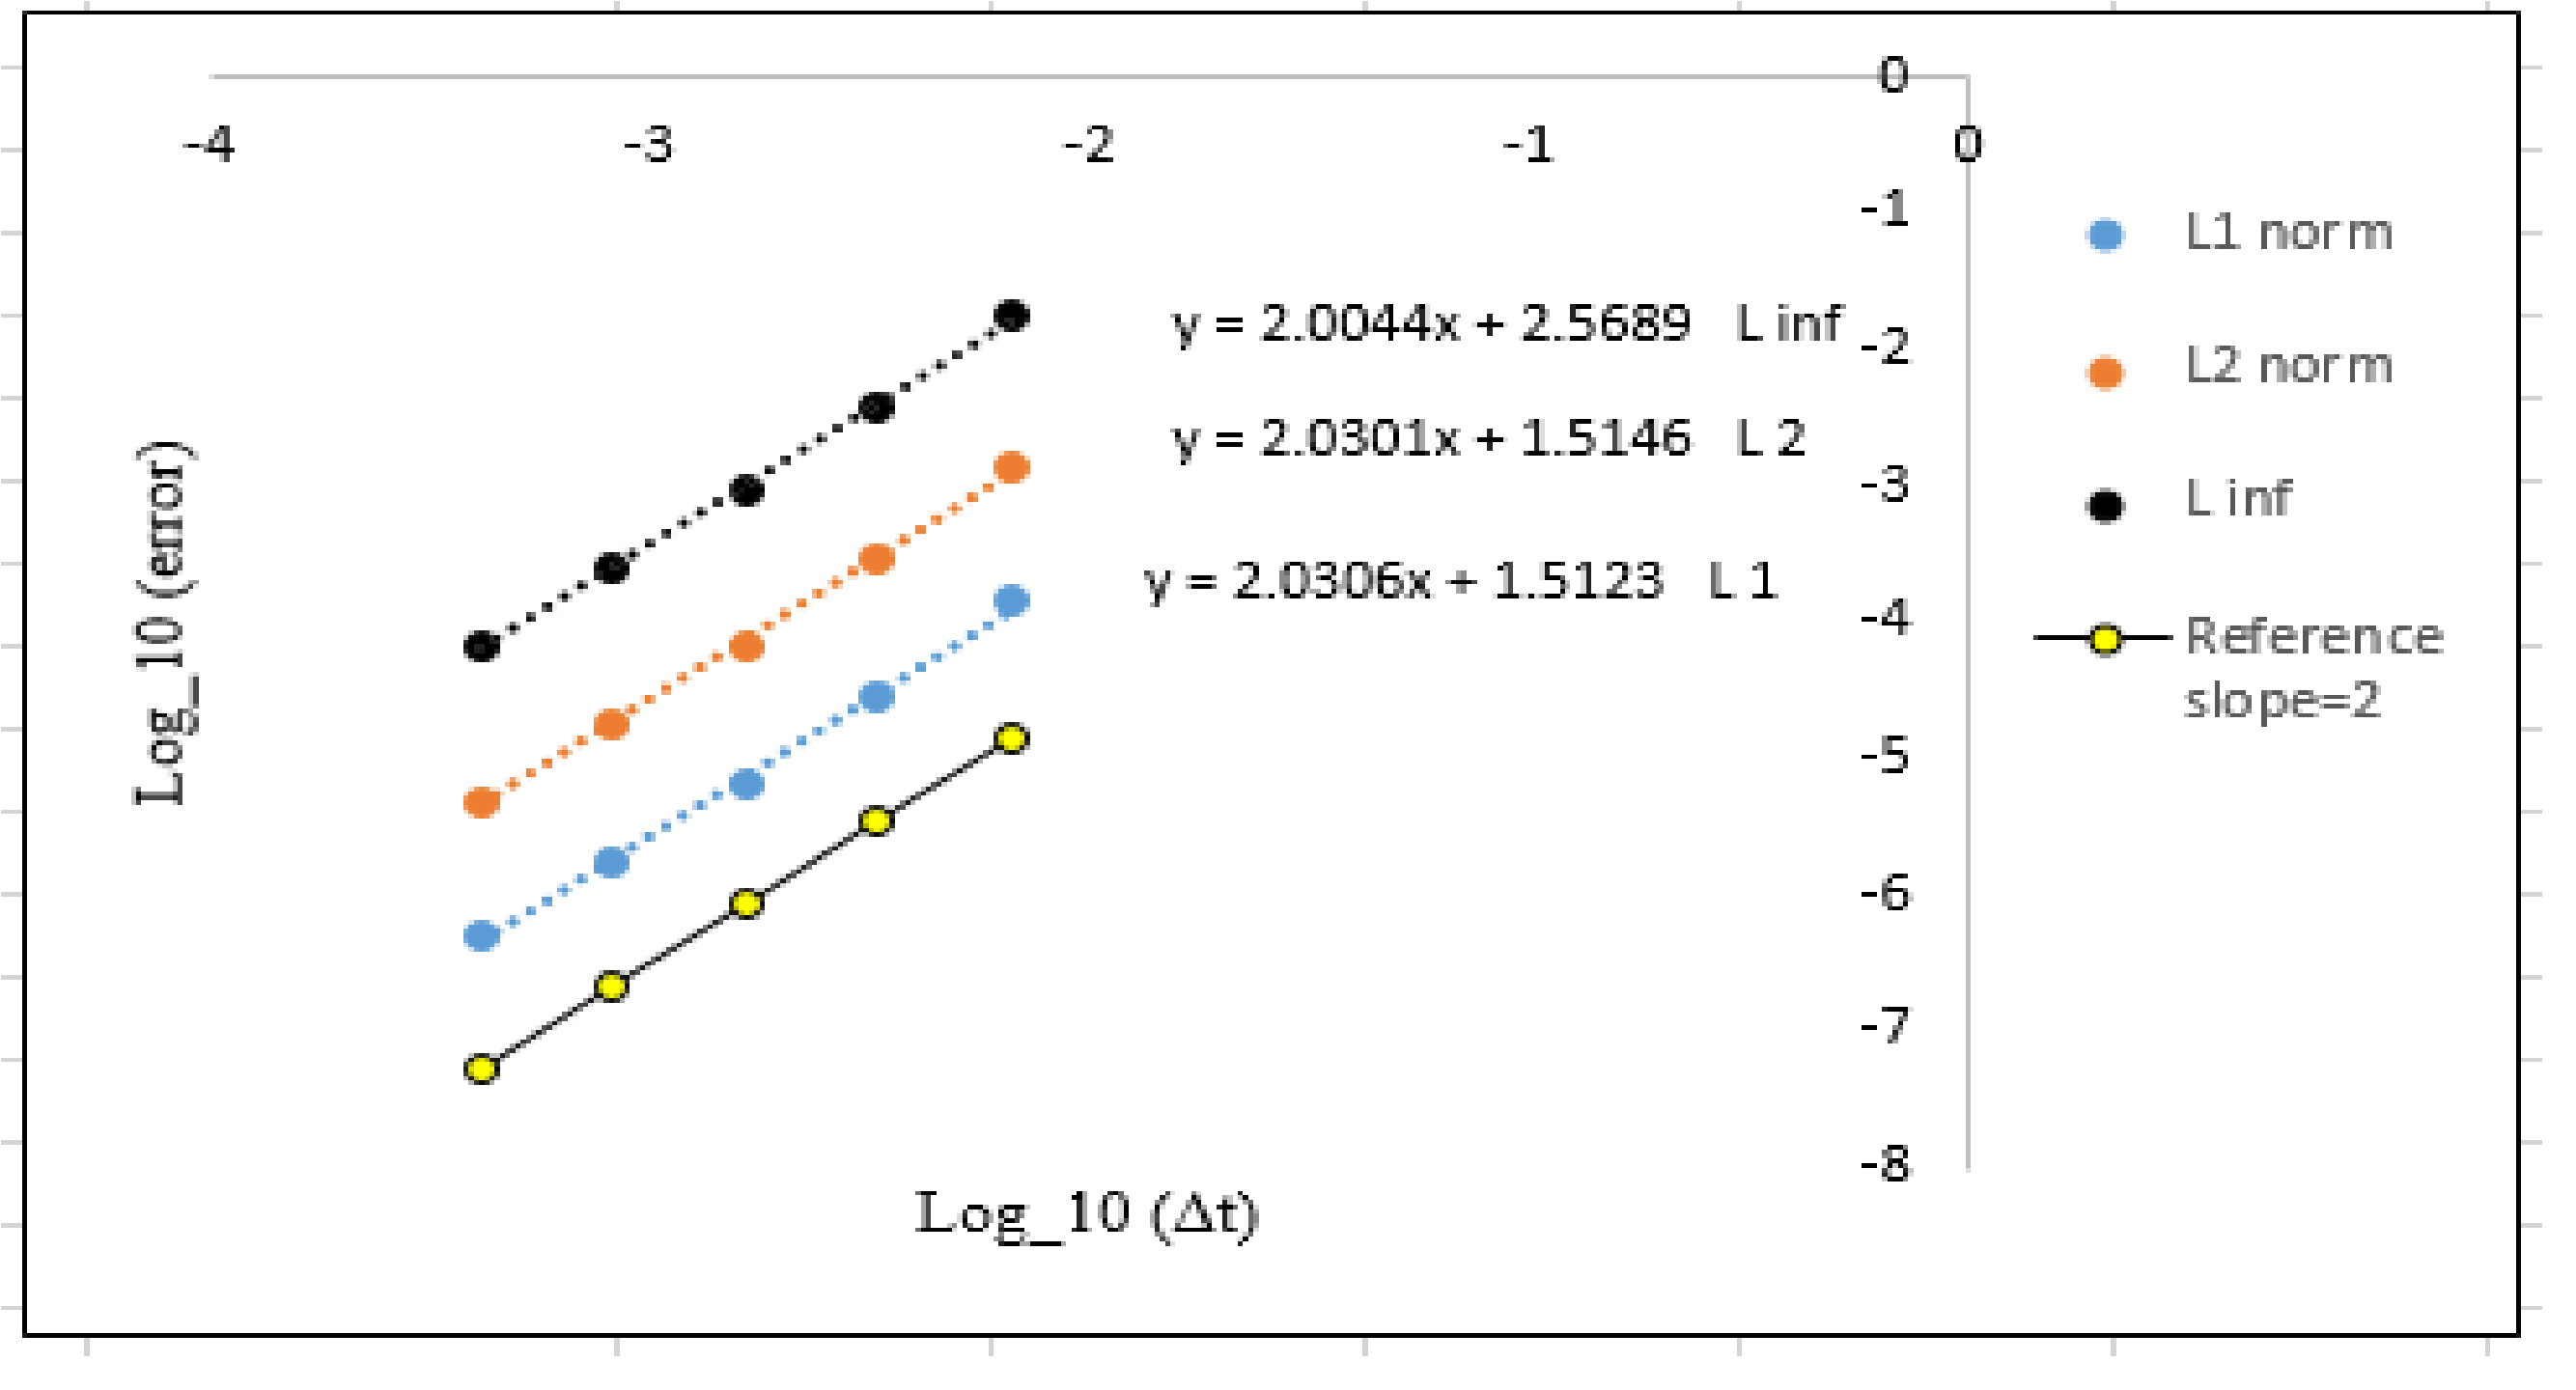
\includegraphics[width=4.5in]{C:/Users/HONGJI/Latex Home directory/Gauge_unf1_np_P_rate.jpg}
		\caption{Log-Log plot of Convergence rate for Pressure Gauge method }\label{fig:6.19b}
	\end{subfigure}
	\caption{Plot of Convergence rates for the Unforced flow problem with Normalised Pressure approach used. Domain: $[-\dfrac{\pi}{4}, \dfrac{\pi}{4}]^2$, time = 0.1 and CFL = 0.05. In each plot, the data points corresponding to grid sizes of 15, 30, 60, 120, 240.}\label{fig:6.16}
\end{figure}

\begin{figure}[H]
	\centering
	\begin{subfigure}[t]{2.5in}
		\centering
		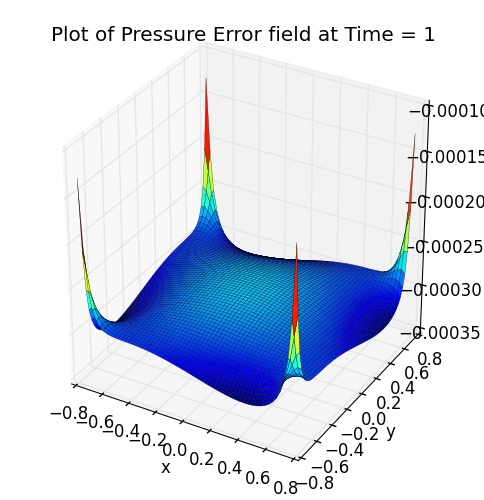
\includegraphics[width=2.5in]{C:/Users/HONGJI/Latex Home directory/Pm1b_unf1_np_P_error_t_1_grid_60.jpg}
		\caption{Pressure error field for $Pm\,1\,(b)$ method}\label{fig:6.19a}		
	\end{subfigure}
	\quad
	\begin{subfigure}[t]{2.5in}
		\centering
		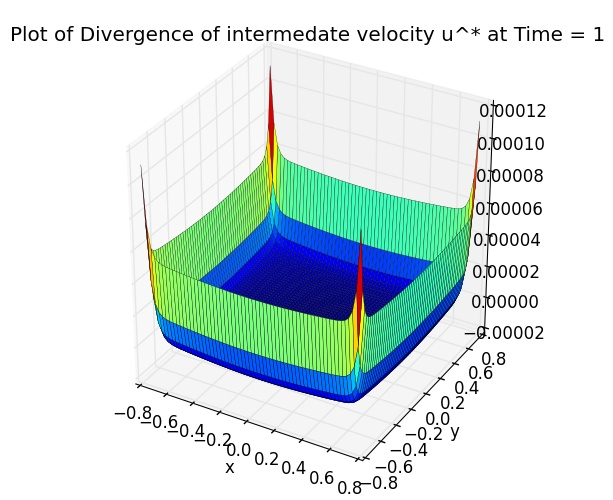
\includegraphics[width=2.5in]{C:/Users/HONGJI/Latex Home directory/Pm1b_unf1_np_div_uvstar_t_1_grid_60.jpg}
		\caption{Divergence of intermediate velocity field $Pm\,1\,(b)$}\label{fig:6.19b}
	\end{subfigure}
	\quad
	\centering
	\begin{subfigure}[t]{2.5in}
		\centering
		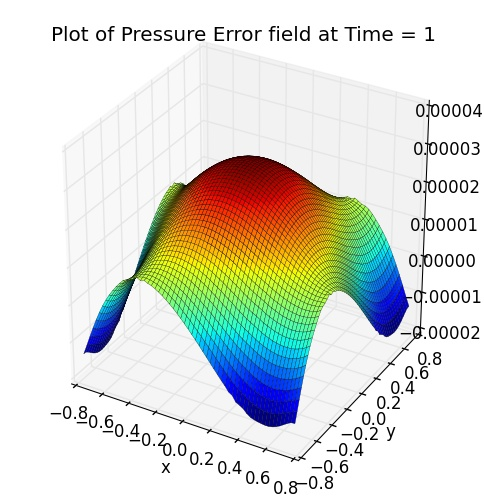
\includegraphics[width=2.5in]{C:/Users/HONGJI/Latex Home directory/Pm2_unf1_np_P_error_t_1_grid_60.jpg}
		\caption{Pressure error field for $Pm\,2$ method}\label{fig:6.19a}		
	\end{subfigure}
	\quad
	\begin{subfigure}[t]{2.5in}
		\centering
		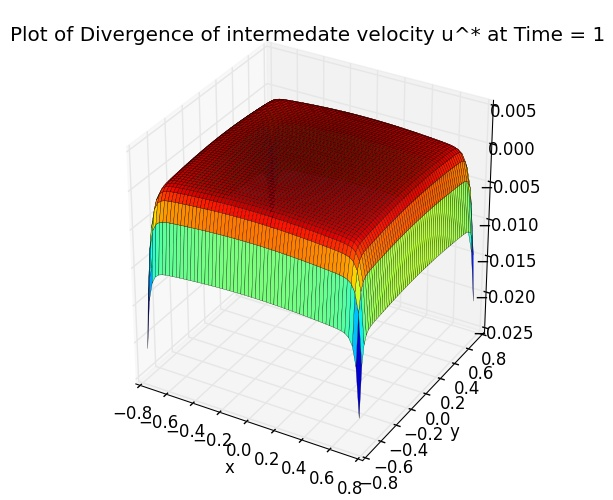
\includegraphics[width=2.5in]{C:/Users/HONGJI/Latex Home directory/Pm2_unf1_np_div_uvstar_t_1_grid_60.jpg}
		\caption{Divergence of intermediate velocity field $Pm\,2$}\label{fig:6.19b}
	\end{subfigure}
	\quad
	\begin{subfigure}[t]{2.5in}
		\centering
		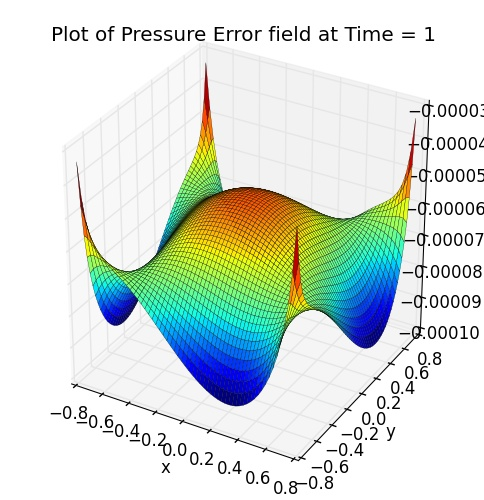
\includegraphics[width=2.5in]{C:/Users/HONGJI/Latex Home directory/Gauge_unf1_P_error_t_1_grid_60.jpg}
		\caption{Pressure error field Gauge method }\label{fig:6.19b}
	\end{subfigure}
	\caption{Plot of Pressure error fields for the Unforced flow problem with Normalised Pressure approach used. Domain: $[-\dfrac{\pi}{4}, \dfrac{\pi}{4}]^2$, time = 0.1 and CFL = 0.05.}\label{fig:6.16}
\end{figure}

\section{Driven cavity flow}
The lack of smoothness is exaggerated in this problem since there is a discontinuity along one of its boundaries. $Pm\,1$ showed reduced order of accuracy.

\begin{itemize}
\item Summary
\end{itemize}
We have observed the following results:
\begin{itemize}
\item We observe that the Gauge method shows fully 2nd order convergence in Pressure in all examples and domains considered whereas Projection methods show a degraded accuracy in some examples. 
\end{itemize}
We observe that the Projection methods depends strongly on the smooth of domain (especially for $Pm\,1\,(b)$). The exact cause of this problem still remains open (\cite{guermond2004error}). This finding is consistent with \emph{Shen et.al} where they have bounded the $L_2$ norm of Pressure error to be only 1.5 order accurate in general domains (e.g. the square domain with Dirichlet boundary conditions we have considered in the Forced flow example). For details of the proof see \cite{guermond2004error, pyo2005normal}.

\begin{itemize}
\item Necessity for accurate boundary condition of the tangential component of the intermediate velocity field ($\textbf{u}^*$)
\end{itemize}
We have observed that second order approximation $\phi^{n+1}$ is needed when computing $\textbf{$\tau$}\cdot\textbf{u}^*$ in the projection step. This is better illustrated in more general domains. The case of periodic channel, all projection methods show 2nd order accuracy in pressure. This is consistent with the predications of error estimates by the normal mode analysis done in previous chapter where a periodic channel domain was considered. We infer that the numerical boundary layers are only partially filtered out in Projection methods. Again if accurate boundary condition for $\textbf{$\tau$}\cdot\textbf{u}^*$ is used (e.g. $Pm\,2$) 2nd order convergence can be restored.


\begin{itemize}
\item Modification to pressure approximation in $Pm\,1\,(b)$
\end{itemize}
We have observed that the inconsistent normal pressure gradient in $Pm\,1\,(b)$ is caused by an inappropriate choice of pressure approximation $q$ used. This introduces non-smooth along the boundary of pressure gradients. This is more evident when the test problems have non-zero pressure gradients. However with a modified $q = 2\phi^{n-1/2} - \phi^{n-3/2}$, we restore fully second order convergence in pressure. The exact reason of this improvement however still subject to more careful considerations.

\begin{figure}[H]
	\centering
	\begin{subfigure}[t]{2.5in}
		\centering
		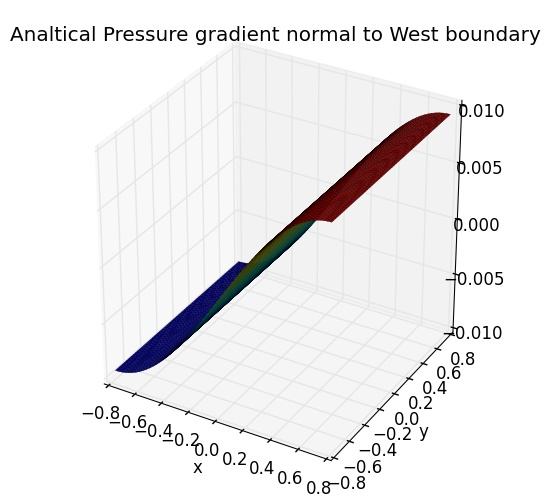
\includegraphics[width=2.5in]{C:/Users/HONGJI/Latex Home directory/Pm1b2_unf1_np_W_NPexgrad_t_1_grid_60.jpg}
		\caption{normal (analytic) pressure gradient to the west boundary}\label{fig:6.19a}		
	\end{subfigure}
	\quad
	\begin{subfigure}[t]{2.5in}
		\centering
		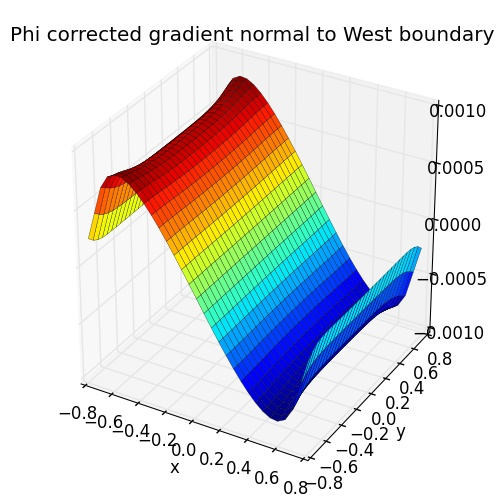
\includegraphics[width=2.5in]{C:/Users/HONGJI/Latex Home directory/Pm1b_unf1_np_W_Nphigrad_t_1_grid_30.jpg}
		\caption{normal (numerical) pressure gradient for $Pm\,1\,(b)$}\label{fig:6.19b}
	\end{subfigure}
	\quad
	\centering
	\begin{subfigure}[t]{2.5in}
		\centering
		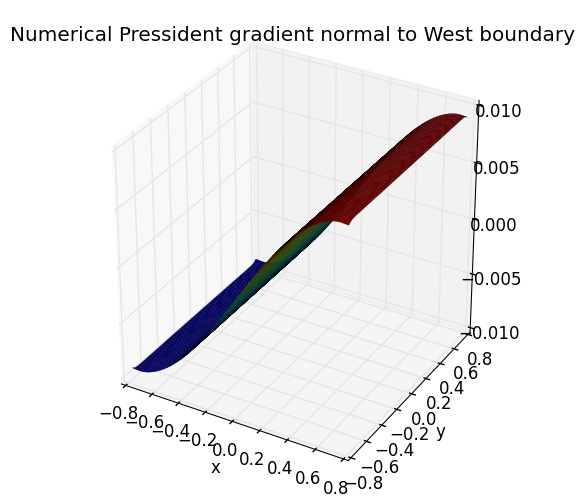
\includegraphics[width=2.5in]{C:/Users/HONGJI/Latex Home directory/Pm1b2_unf1_np_W_Npf_t_1_grid_60.jpg}
		\caption{normal (numerical) pressure gradient for $Pm\,1\,(b)$ modified}\label{fig:6.19a}		
	\end{subfigure}
	\quad
	\begin{subfigure}[t]{2.5in}
		\centering
		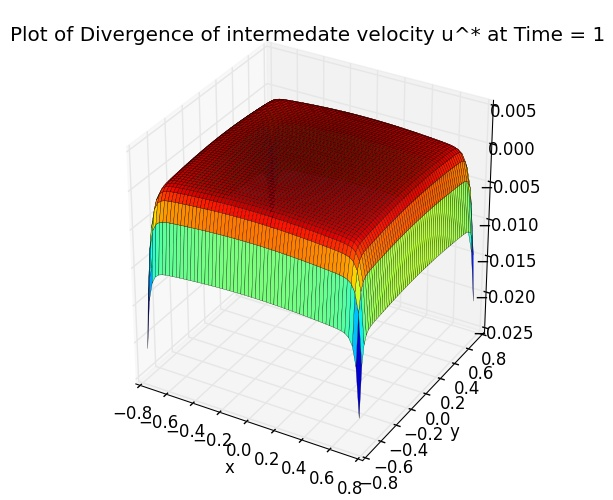
\includegraphics[width=2.5in]{C:/Users/HONGJI/Latex Home directory/Pm2_unf1_np_div_uvstar_t_1_grid_60.jpg}
		\caption{Divergence of intermediate velocity field $Pm\,2$}\label{fig:6.19b}
	\end{subfigure}
	\quad
	\begin{subfigure}[t]{2.5in}
		\centering
		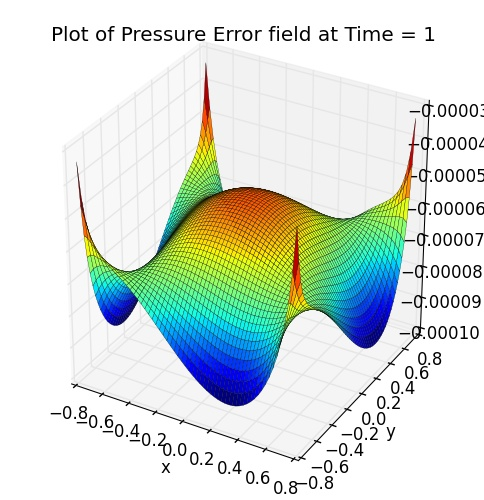
\includegraphics[width=2.5in]{C:/Users/HONGJI/Latex Home directory/Gauge_unf1_P_error_t_1_grid_60.jpg}
		\caption{Pressure error field Gauge method }\label{fig:6.19b}
	\end{subfigure}
	\caption{Plot of Pressure error fields for the Unforced flow problem with Normalised Pressure approach used. Domain: $[-\dfrac{\pi}{4}, \dfrac{\pi}{4}]^2$, time = 0.1 and CFL = 0.05.}\label{fig:6.16}
\end{figure}